\newglossaryentry{Charles D. Moore}
{
  name={Charles D. Moore},
  description={Charles D. Moore, is the inventor of the forth programming language.}
}

\chapter{Results}
\label{chap:Results}

In this chapter, I will introduce the chosen forth software. Afterwards, I will manually or semi automatically produce the graphics according to the selected Visualization methods.

\section{The software under investigation: Brainless}

Brainless\footnote{Brainless verion 0.1.2 is used, the source code can be optained on \url{http://sourceforge.net/projects/forth-brainless/}} is chess-playing program written in ANS Forth. The source code consists of several files with an overall size\footnote{The command to calculate the size was \emph{find . -name '*.fs' -maxdepth 1 | xargs wc -l}} of about 139497 bytes and 4108 lines of code\footnote{The command used to count the lines of code, was \emph{find . -name '*.fs' -maxdepth 1 | xargs wc -l}}.
This measure is somehow controversial, but since the files contain only a short header and are formatted in the usual manner, it seems appropriate for comparison. The code is organized in a flat structure, one directory, 30 files and 663 words. There is only on custom word list defined. Thus the visualization of a word list hierarchy makes obviously little sense and is left out in the following sections. Almost all files are included at the beginning of the execution.

The other software, I took into consideration, was brew\footnote{brew version 0.2.0 was used. The source code can be obtained on \url{http://www.robertepprecht.ch/brew/index.html}}. Brew is a 'playground for evolutionary programming', as the author calls it. Due to its size of 1062857 bytes and 36801 lines of code, this project seem to large to analyze manually in a reasonable time.

For the following figures, I used a snapshot of an execution trace.
Since the calculations of the computer moves produce a huge amount of word executions, the example trace, was created by making only the player move: \emph{d2 d3 m} \keys{\return}. The snapshot contains all word executions after and including the execution of the word \emph{m}. It consists of 4709 word executions. \ref{fig:brainless_before_m} and \ref{fig:brainless_after_m} show the state of the game before and after entering \emph{d2 d3 m} \keys{\return}.

\begin{figure}[p]
    \centering
    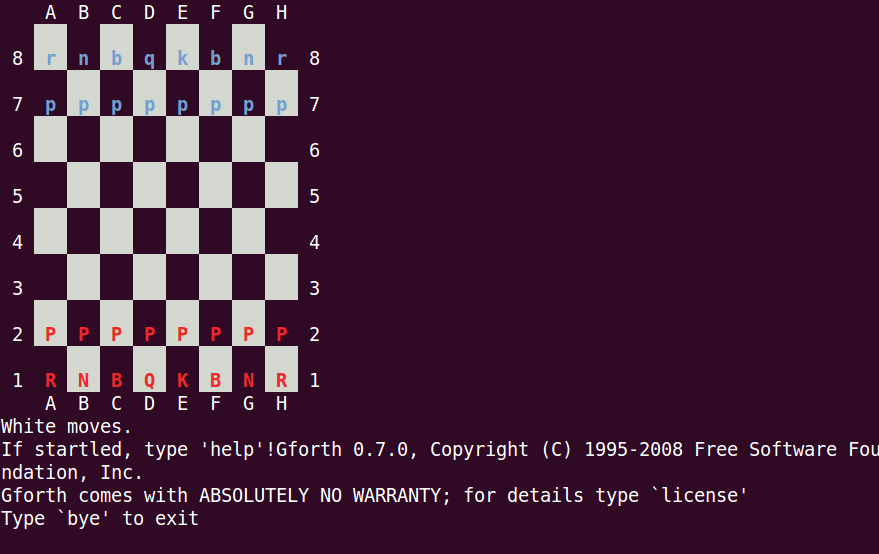
\includegraphics[scale=0.4]{graphics/brainless_before.png}
    \caption{State of the game before entering \emph{d2 d3 m}}
    \label{fig:brainless_before_m}
\end{figure}

\begin{figure}[p]
    \centering
    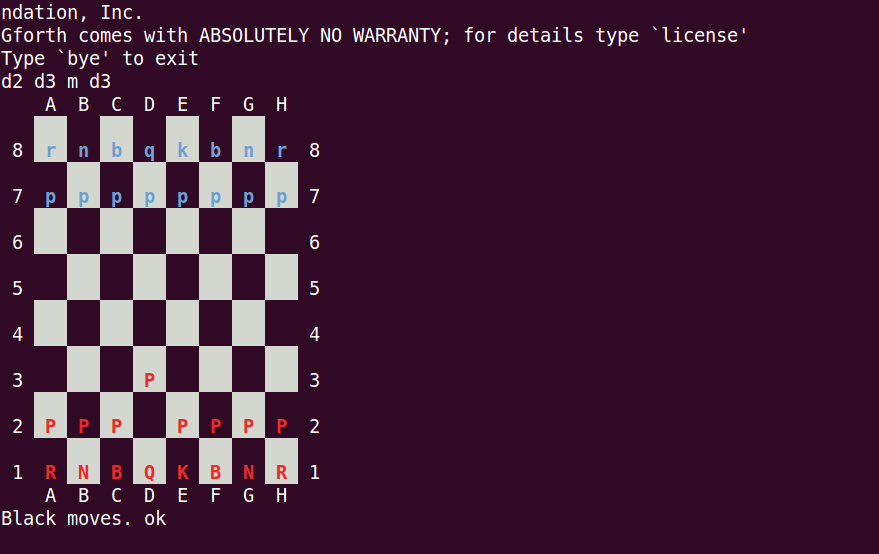
\includegraphics[scale=0.4]{graphics/brainless_after.png}
    \caption{State of the game after entering \emph{d2 d3 m}}
    \label{fig:brainless_after_m}
\end{figure}

\section{The application of the previously presented methods}

\subsection*{Hierarchical edge bundles}

Figure \ref{fig:hierarchic_edge_bundle} shows the trace snapshot mentioned before in a \emph{hierarchic edge bundle}.

\begin{figure}[p]
    \centering
    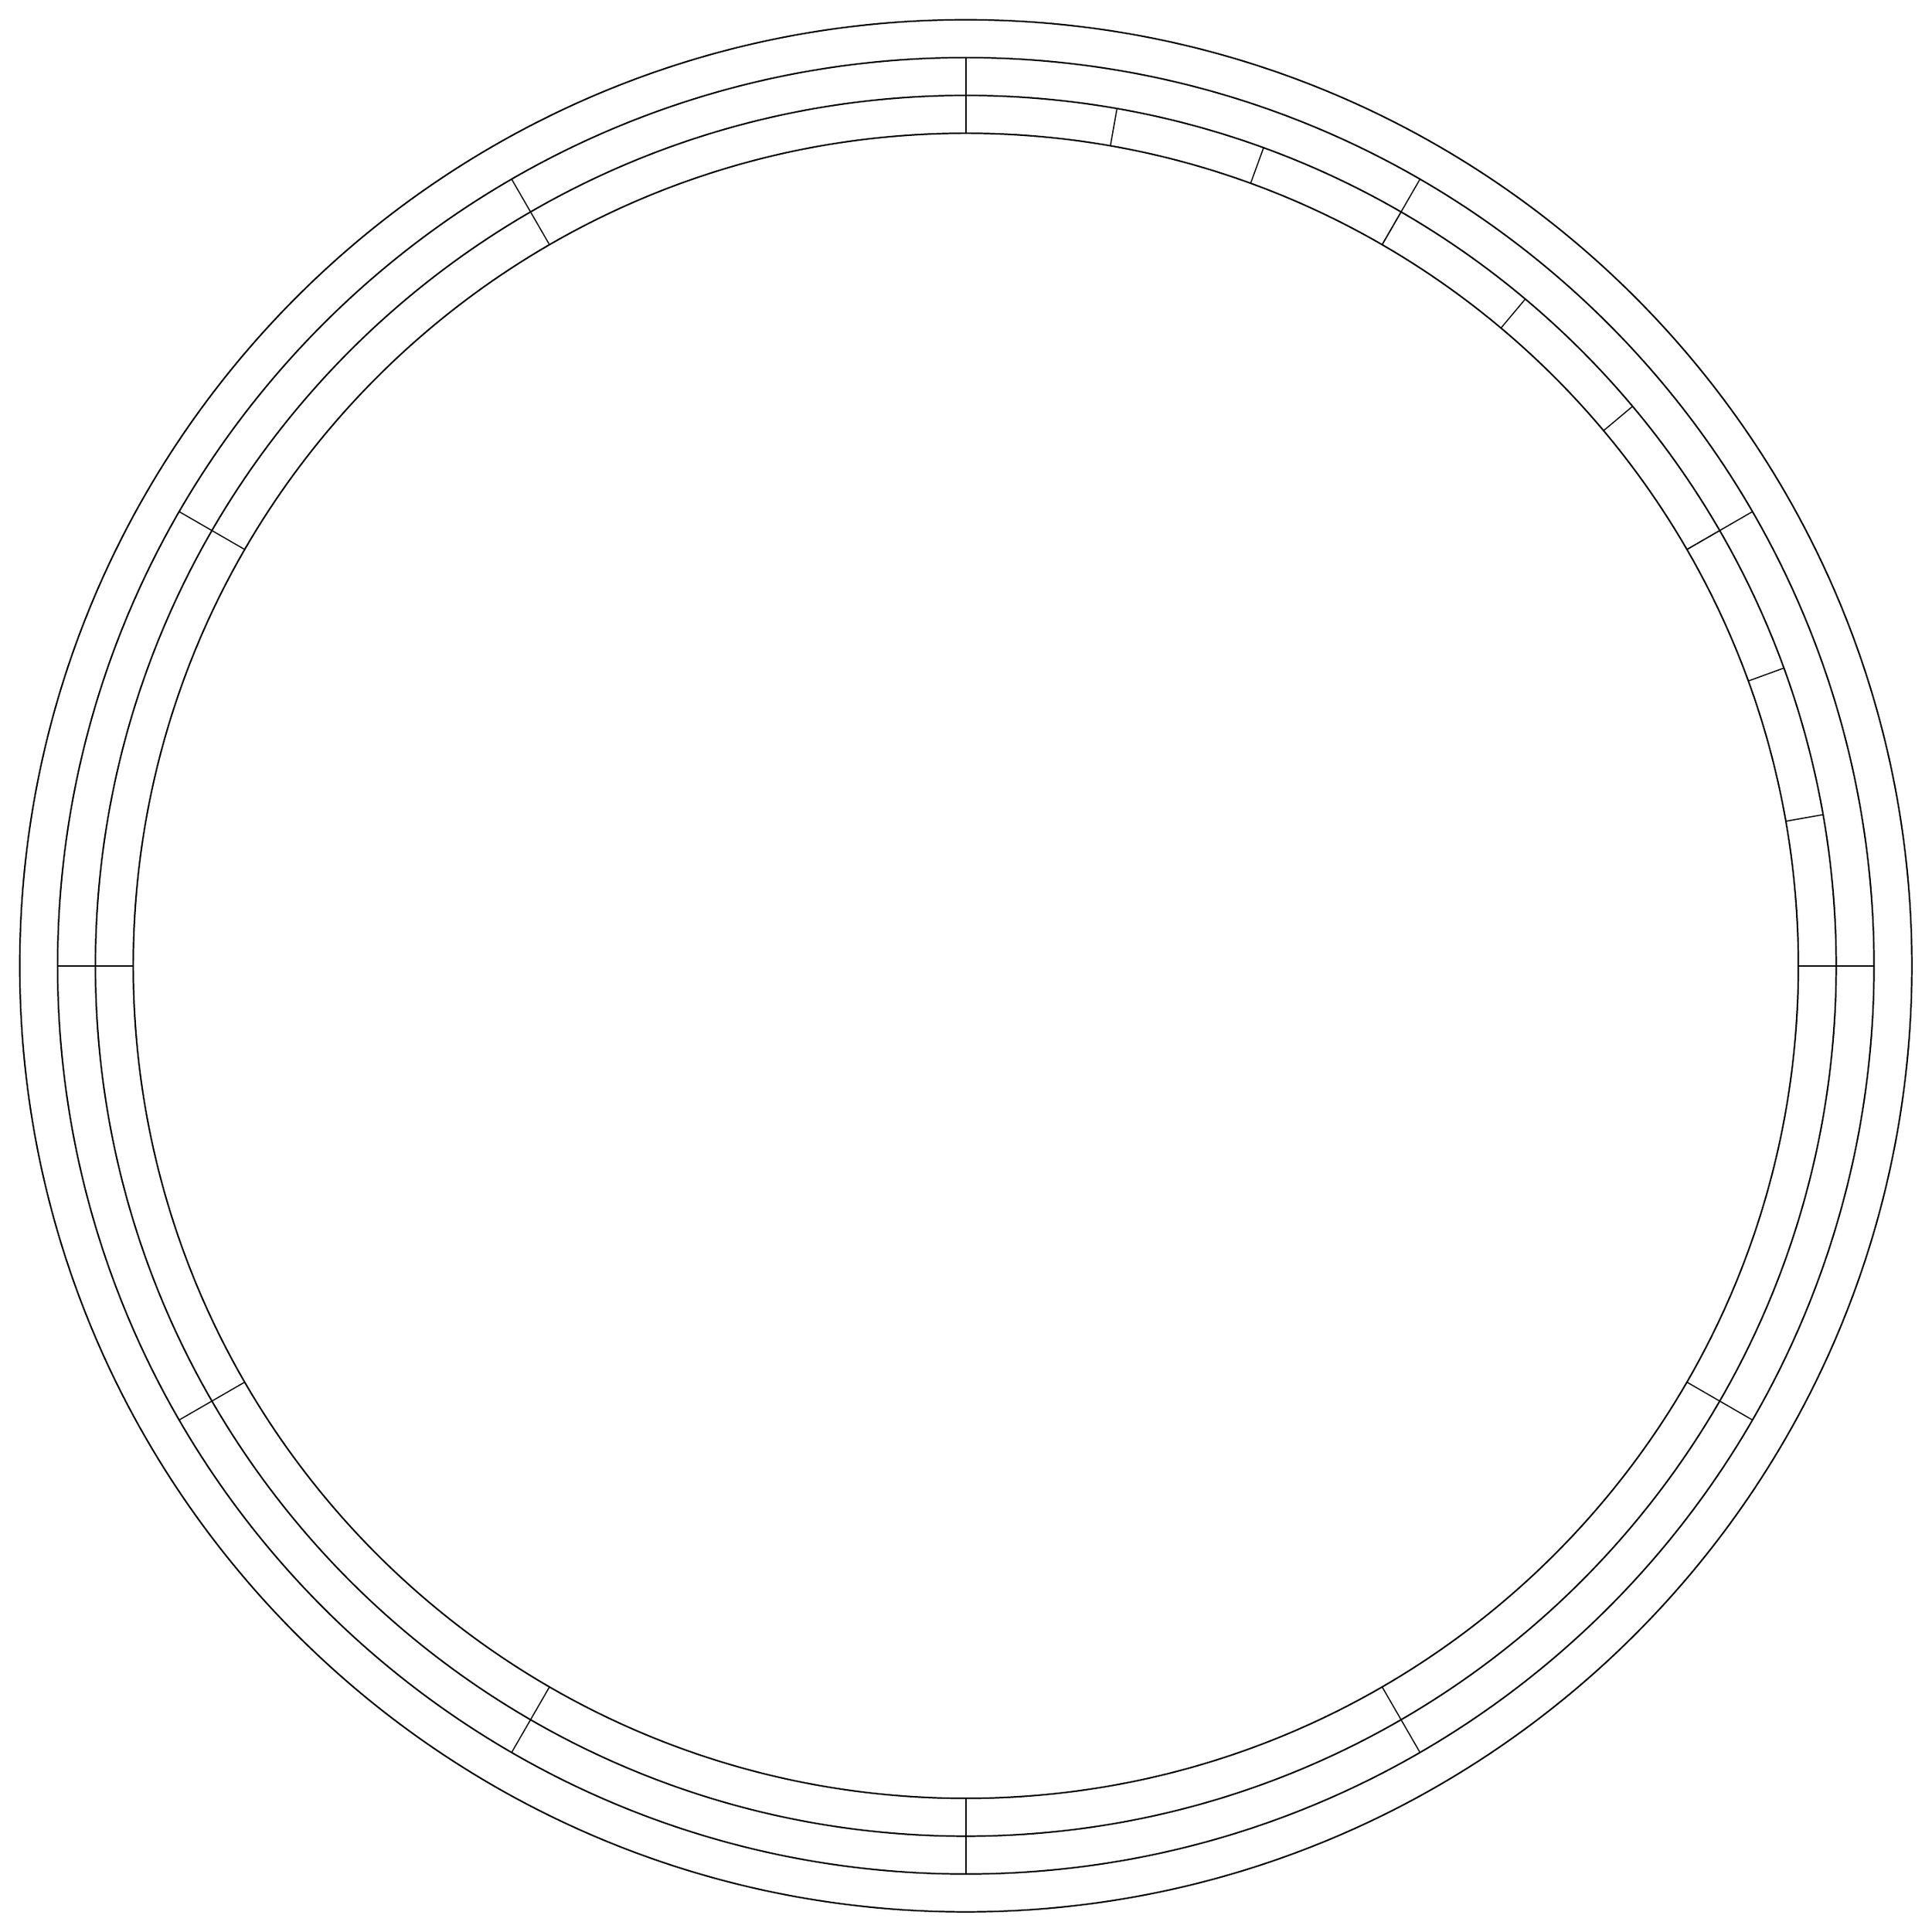
\begin{tikzpicture}[>=latex,font=\sffamily,semithick,scale=1.75]

	% outer ring
	\draw [thick] (0,0) circle (10);
	\draw [thick] (0,0) circle (9.6);

	% 2. outer ring
    \foreach \angle in {90, 60, ..., -90}
        \draw (\angle:9.6) -- (\angle-180:9.6);
    \draw [thick] (0,0) circle (9.2);

	% 3. outer ring
	% section 90-60
	\foreach \angle in {90, 80, ..., 0}
		\draw (\angle:9.2) -- (\angle-180:0);
	% section 60-30
	%\foreach \angle in {90, 60, ..., -90}
	%	\draw (\angle:9.2) -- (\angle-180:0);
	% section 30-0
	%\foreach \angle in {30, 0}
	%	\draw (\angle:9.2) -- (\angle-180:0);
	\draw [thick,fill=white] (0,0) circle (8.8);

%    \node [circle,thick,fill=white,draw=black,align=center,minimum size=5cm] at (0,0) {};
%    (Head.west);
\end{tikzpicture}
    \caption{Hierarchic edge bundle of Brainless after \emph{d2 d3 m}}
    \label{fig:hierarchic_edge_bundle}
\end{figure}


\subsection*{Information murals and massive sequence view}

Figure \ref{fig:massive_sequence_view} shows the trace snapshot in a \emph{massive sequence view}. It is easy to identify certain steps of the program execution like the drawing part at the end of the trace(interaction withing drawing.fs) and the file writing part(interaction within epd.fs), if one know the words contained in those files. But it also clearly shows the lack of interactivity. Without filtering, zooming, on-demand information on words(references to source code) and of course expressive naming, it still remains hard to map the phases of the trace to behavior. Besides these concerns, the massive sequence view seems to be well applicable to forth program traces.

\begin{figure}[p]
    \centering
    \begin{tikzpicture}[>=latex,font=\sffamily,semithick,scale=2,] % 0.8 fits into latex doc(width only)

\tikzstyle{every node}=[font=\large] %\ŧiny for 0.8 and 20

\def \width { 25 } %20 fits into latex doc(width only)
\pgfmathsetmacro {\dirHeight} { -1 } %
\pgfmathsetmacro {\fileHeight} { 3 }
\pgfmathsetmacro {\wordHeight} { 1 }

\def \interactionHeight { 0.0125 }
\def \wordCount { 663 }

\pgfmathsetmacro {\wordWidth } { \width / \wordCount } % 30 / 663 = 0.045248869


\edef \intRowIdx { 0 }
\newcommand{ \incrementRowIdx } {

	\pgfmathparse { \intRowIdx + 1 } \xdef \intRowIdx { \pgfmathresult }

	%also redefine macro
	\pgfmathsetmacro {\intStartY } { \dirHeight - \fileHeight - \wordHeight - \interactionHeight * \intRowIdx }
	\pgfmathsetmacro {\intEndY } { \intStartY - \interactionHeight }
}

\pgfmathsetmacro {\intStartY } { \dirHeight - \fileHeight - \wordHeight - \interactionHeight * \intRowIdx }
\pgfmathsetmacro {\intEndY } { \intStartY - \interactionHeight }

\newcommand{\drawInteraction}[2]{
	
	\pgfmathparse{#1}
    \pgfmathsetmacro{\from}{\pgfmathresult}
	\pgfmathparse{#2}
    \pgfmathsetmacro{\to}{\pgfmathresult}

	\ifdim \from pt < \to pt

		\def \leftColor{green}
		\def \rightColor{red}	

	\else

		\def \leftColor{red}
		\def \rightColor{green}
		
	\fi

	\fill [left color= \leftColor, right color= \rightColor] 
		({#1}, \intStartY) rectangle ({#2}, \intEndY)-- cycle;

	\incrementRowIdx
}

% file coord offset
\pgfmathsetmacro{\boardFs}				{  									  0 * \wordWidth }
\pgfmathsetmacro{\drawingFs}		{ \boardFs				+ 51 * \wordWidth }
\pgfmathsetmacro{\environFs}			{ \drawingFs		+ 24 * \wordWidth }
\pgfmathsetmacro{\benchmarkFs}	{ \environFs			+ 14 * \wordWidth }
\pgfmathsetmacro{\epdFs}					{ \benchmarkFs	+ 22 * \wordWidth }
\pgfmathsetmacro{\evalFs}				{ \epdFs					+ 25 * \wordWidth }
\pgfmathsetmacro{\flyevalFs}			{ \evalFs					+ 26 * \wordWidth }
\pgfmathsetmacro{\hashFs}				{ \flyevalFs			+ 19 * \wordWidth }
\pgfmathsetmacro{\historyFs}			{ \hashFs				+ 17 * \wordWidth }
\pgfmathsetmacro{\killerFs}				{ \historyFs			+   6 * \wordWidth }
\pgfmathsetmacro{\moveconvFs}		{ \killerFs				+ 43 * \wordWidth }
\pgfmathsetmacro{\movegenFs}		{ \moveconvFs		+ 21 * \wordWidth }
\pgfmathsetmacro{\movesFs}			{ \movegenFs		+ 63 * \wordWidth }
\pgfmathsetmacro{\nullFs}					{ \movesFs			+ 90 * \wordWidth }
\pgfmathsetmacro{\optionsFs}			{ \nullFs					+   5 * \wordWidth }
\pgfmathsetmacro{\profilerFs}			{ \optionsFs			+   0 * \wordWidth }
\pgfmathsetmacro{\quiescenceFs}	{ \profilerFs			+ 13 * \wordWidth }
\pgfmathsetmacro{\repeatFs}			{ \quiescenceFs	+   7 * \wordWidth }
\pgfmathsetmacro{\searchdefsFs}	{ \repeatFs			+   4 * \wordWidth }
\pgfmathsetmacro{\searchFs}			{ \searchdefsFs	+   4 * \wordWidth }
\pgfmathsetmacro{\sglmovesFs}		{ \searchFs			+ 36 * \wordWidth }
\pgfmathsetmacro{\sortingFs}			{ \sglmovesFs		+ 14 * \wordWidth }
\pgfmathsetmacro{\stringFs}				{ \sortingFs			+   6 * \wordWidth }
\pgfmathsetmacro{\testsFs}				{ \stringFs				+ 18 * \wordWidth }
\pgfmathsetmacro{\threatsFs}			{ \testsFs				+ 11 * \wordWidth }
\pgfmathsetmacro{\tmovegenFs}		{ \threatsFs			+ 35 * \wordWidth }
\pgfmathsetmacro{\ttableFs}				{ \tmovegenFs		+ 27 * \wordWidth }
\pgfmathsetmacro{\tuiFs}					{ \ttableFs				+ 14 * \wordWidth }
\pgfmathsetmacro{\utilsFs}				{ \tuiFs					+ 29 * \wordWidth }
\pgfmathsetmacro{\brainlessFs}		{ \utilsFs				+ 15 * \wordWidth }

% word coord offset to the middle of the word section
\newcommand{ \wordOffset }[1] {
	(#1 * \wordWidth - \wordWidth / 2)
}

% word section coords; the index starts at 0
\pgfmathsetmacro{\addMove } 															{ \movesFs + \wordOffset{28} }
\pgfmathsetmacro{\appendMoves } 												{ \movegenFs + \wordOffset{43} }
\pgfmathsetmacro{\appendMoveToSan } 										{ \moveconvFs + \wordOffset{17} }
\pgfmathsetmacro{\bishopMoves } 													{ \movegenFs + \wordOffset{19} }
\pgfmathsetmacro{\bishopThreatensThroughQ } 						{ \threatsFs + \wordOffset{30} }
\pgfmathsetmacro{\bishopThreatsDeltaEval } 								{ \flyevalFs + \wordOffset{2} }
\pgfmathsetmacro{\bishopXyQ } 														{ \boardFs + \wordOffset{11} }
\pgfmathsetmacro{\blackFieldAttr } 												{ \drawingFs + \wordOffset{12} }
\pgfmathsetmacro{\blackPiece } 														{ \boardFs + \wordOffset{29} }
\pgfmathsetmacro{\blackPieceAttr } 												{ \drawingFs + \wordOffset{15} }
\pgfmathsetmacro{\DBoard } 															{ \drawingFs + \wordOffset{32} }
\pgfmathsetmacro{\DBoardLine } 													{ \drawingFs + \wordOffset{30} }
\pgfmathsetmacro{\captureMoveQ } 												{ \movesFs + \wordOffset{33} }
\pgfmathsetmacro{\castleFar } 															{ \movegenFs + \wordOffset{16} }
\pgfmathsetmacro{\castleMoveQ } 													{ \movesFs + \wordOffset{34} }
\pgfmathsetmacro{\castleNear } 														{ \movegenFs + \wordOffset{15} }
\pgfmathsetmacro{\HCharacters } 													{ \stringFs + \wordOffset{6} }
\pgfmathsetmacro{\checkQ } 															{ \threatsFs + \wordOffset{16} }
\pgfmathsetmacro{\currChar } 															{ \stringFs + \wordOffset{11} }
\pgfmathsetmacro{\deltaEval } 															{ \flyevalFs + \wordOffset{6} }
\pgfmathsetmacro{\toDeltaXy } 														{ \boardFs + \wordOffset{10} }
\pgfmathsetmacro{\deltaXyToDirection } 										{ \boardFs + \wordOffset{15} }
\pgfmathsetmacro{\QDirection } 														{ \boardFs + \wordOffset{40} }
\pgfmathsetmacro{\displayMove } 													{ \moveconvFs + \wordOffset{21} }
\pgfmathsetmacro{\doMove } 															{ \movesFs + \wordOffset{87} }
\pgfmathsetmacro{\doMoveUndoInfo } 											{ \movesFs + \wordOffset{86} }
\pgfmathsetmacro{\BdoNormalMoveB } 										{ \movesFs + \wordOffset{63} }
\pgfmathsetmacro{\doNormalMove } 												{ \movesFs + \wordOffset{64} }
\pgfmathsetmacro{\emptyQ } 															{ \boardFs + \wordOffset{33} }
\pgfmathsetmacro{\QEpdAppendToFile } 										{ \epdFs + \wordOffset{26} }
\pgfmathsetmacro{\epdAppendToFile } 											{ \epdFs + \wordOffset{24} }
\pgfmathsetmacro{\epdCloseFile } 													{ \epdFs + \wordOffset{18} }
\pgfmathsetmacro{\epdWriteBoard } 												{ \epdFs + \wordOffset{2} }
\pgfmathsetmacro{\epdWriteBoardLine } 										{ \epdFs + \wordOffset{1} }
\pgfmathsetmacro{\epdWriteCastle } 												{ \epdFs + \wordOffset{4} }
\pgfmathsetmacro{\epdWriteEp } 													{ \epdFs + \wordOffset{5} }
\pgfmathsetmacro{\epdWriteParty } 												{ \epdFs + \wordOffset{3} }
\pgfmathsetmacro{\epdWriteToFile } 												{ \epdFs + \wordOffset{23} }
\pgfmathsetmacro{\evalKnightThreats } 										{ \evalFs + \wordOffset{4} }
\pgfmathsetmacro{\evalPawnThreats } 											{ \evalFs + \wordOffset{3} }
\pgfmathsetmacro{\evalPut } 															{ \flyevalFs + \wordOffset{7} }
\pgfmathsetmacro{\evalRemove } 													{ \flyevalFs + \wordOffset{8} }
\pgfmathsetmacro{\evalStraightThreats } 										{ \evalFs + \wordOffset{2} }
\pgfmathsetmacro{\evalThreat } 														{ \evalFs + \wordOffset{1} }
\pgfmathsetmacro{\fieldAttr } 															{ \drawingFs + \wordOffset{13} }
\pgfmathsetmacro{\DFieldSlice } 														{ \drawingFs + \wordOffset{28} }
\pgfmathsetmacro{\fieldSpaces } 														{ \drawingFs + \wordOffset{17} }
\pgfmathsetmacro{\fileExistsQ } 														{ \utilsFs + \wordOffset{8} }
\pgfmathsetmacro{\QFindMove } 													{ \tuiFs + \wordOffset{18} }
\pgfmathsetmacro{\findMove } 														{ \movesFs + \wordOffset{39} }
\pgfmathsetmacro{\flyEvalMoves } 													{ \flyevalFs + \wordOffset{18} }
\pgfmathsetmacro{\flyEvalNormalMove } 										{ \flyevalFs + \wordOffset{11} }
\pgfmathsetmacro{\forgetMoves } 													{ \movesFs + \wordOffset{38} }
\pgfmathsetmacro{\forgetPosition } 												{ \repeatFs + \wordOffset{3} }
\pgfmathsetmacro{\BgenerateMovesB } 										{ \movegenFs + \wordOffset{42} }
\pgfmathsetmacro{\generateMoves } 												{ \movegenFs + \wordOffset{46} }
\pgfmathsetmacro{\BgenerateMovesFromB } 								{ \movegenFs + \wordOffset{39} }
\pgfmathsetmacro{\BgenerateMoveToB } 										{ \movegenFs + \wordOffset{38} }
\pgfmathsetmacro{\BgenerateMoveToNocheckB } 					{ \movegenFs + \wordOffset{36} }
\pgfmathsetmacro{\getMove } 															{ \movesFs + \wordOffset{23} }
\pgfmathsetmacro{\getMoveClass } 												{ \movesFs + \wordOffset{30} }
\pgfmathsetmacro{\getMoveSquares } 											{ \movesFs + \wordOffset{31} }
\pgfmathsetmacro{\getOrig } 															{ \movesFs + \wordOffset{26} }
\pgfmathsetmacro{\getPieceMasked } 											{ \boardFs + \wordOffset{43} }
\pgfmathsetmacro{\getTarget } 														{ \movesFs + \wordOffset{29} }
\pgfmathsetmacro{\hashFarMovedPawn } 									{ \hashFs + \wordOffset{34} }
\pgfmathsetmacro{\hashPiece } 														{ \hashFs + \wordOffset{31} }
\pgfmathsetmacro{\hashSquare } 													{ \hashFs + \wordOffset{32} }
\pgfmathsetmacro{\Dhborder } 														{ \drawingFs + \wordOffset{31} }
\pgfmathsetmacro{\histRecord } 														{ \historyFs + \wordOffset{2} }
\pgfmathsetmacro{\QInString } 														{ \stringFs + \wordOffset{10} }
\pgfmathsetmacro{\inStringQ } 														{ \stringFs + \wordOffset{9} }
\pgfmathsetmacro{\isString } 															{ \stringFs + \wordOffset{4} }
\pgfmathsetmacro{\QKingEval } 														{ \evalFs + \wordOffset{15} }
\pgfmathsetmacro{\kingMove } 														{ \movegenFs + \wordOffset{12} }
\pgfmathsetmacro{\kingMoves } 														{ \movegenFs + \wordOffset{22} }
\pgfmathsetmacro{\kingSquare } 														{ \boardFs + \wordOffset{29} }
\pgfmathsetmacro{\knightEval } 														{ \evalFs + \wordOffset{21} }
\pgfmathsetmacro{\knightMoves } 													{ \movegenFs + \wordOffset{18} }
\pgfmathsetmacro{\look } 																	{ \tuiFs + \wordOffset{2} }
\pgfmathsetmacro{\m } 																		{ \tuiFs + \wordOffset{20} }
\pgfmathsetmacro{\mightCauseCheckQ } 										{ \threatsFs + \wordOffset{34} }
\pgfmathsetmacro{\moveC } 																{ \movesFs + \wordOffset{22} }
\pgfmathsetmacro{\moveS } 																{ \movesFs + \wordOffset{21} }
\pgfmathsetmacro{\moveF } 																{ \movesFs + \wordOffset{20} }
\pgfmathsetmacro{\moved } 																{ \boardFs + \wordOffset{26} }
\pgfmathsetmacro{\moves } 																{ \movesFs + \wordOffset{19} }
\pgfmathsetmacro{\moveToSan } 														{ \moveconvFs + \wordOffset{18} }
\pgfmathsetmacro{\movesExistQ } 													{ \movegenFs + \wordOffset{63} }
\pgfmathsetmacro{\moveSquares } 													{ \movesFs + \wordOffset{14} }
\pgfmathsetmacro{\moveToString } 												{ \moveconvFs + \wordOffset{20} }
\pgfmathsetmacro{\BmoveToExistsQB } 										{ \movegenFs + \wordOffset{62} }
\pgfmathsetmacro{\BmoveToExistsQNocheckB } 						{ \movegenFs + \wordOffset{60} }
\pgfmathsetmacro{\myPieceQ } 														{ \boardFs + \wordOffset{37} }
\pgfmathsetmacro{\newMoves } 														{ \movesFs + \wordOffset{37} }
\pgfmathsetmacro{\newString } 														{ \stringFs + \wordOffset{2} }
\pgfmathsetmacro{\nextChar } 															{ \stringFs + \wordOffset{7} }
\pgfmathsetmacro{\noAttr } 																{ \drawingFs + \wordOffset{10} }
\pgfmathsetmacro{\opponentQ } 													{ \boardFs + \wordOffset{35} }
\pgfmathsetmacro{\opponentBishopQ } 										{ \threatsFs + \wordOffset{4} }
\pgfmathsetmacro{\opponentKingSquare } 									{ \boardFs + \wordOffset{4} }
\pgfmathsetmacro{\opponentKnightQ } 										{ \threatsFs + \wordOffset{2} }
\pgfmathsetmacro{\opponentMoveOrig } 										{ \movesFs + \wordOffset{12} }
\pgfmathsetmacro{\opponentMoveTarget } 									{ \movesFs + \wordOffset{9} }
\pgfmathsetmacro{\opponentPawnQ } 											{ \threatsFs + \wordOffset{1} }
\pgfmathsetmacro{\opponentPieces } 											{ \boardFs + \wordOffset{47} }
\pgfmathsetmacro{\opponentRookQ } 											{ \threatsFs + \wordOffset{5} }
\pgfmathsetmacro{\otherParty } 														{ \boardFs + \wordOffset{17} }
\pgfmathsetmacro{\DParty } 																{ \tuiFs + \wordOffset{1} }
\pgfmathsetmacro{\pawnQ } 																{ \boardFs + \wordOffset{39} }
\pgfmathsetmacro{\pawnDeltaEval } 												{ \flyevalFs + \wordOffset{4} }
\pgfmathsetmacro{\QPawnEval } 														{ \evalFs + \wordOffset{14} }
\pgfmathsetmacro{\pawnFarMove } 												{ \movegenFs + \wordOffset{4} }
\pgfmathsetmacro{\pawnMoves } 													{ \movegenFs + \wordOffset{17} }
\pgfmathsetmacro{\pawnNormalMove } 										{ \movegenFs + \wordOffset{7} }
\pgfmathsetmacro{\pawnRowEval } 												{ \evalFs + \wordOffset{13} }
\pgfmathsetmacro{\pawnStrikeMove } 											{ \movegenFs + \wordOffset{8} }
\pgfmathsetmacro{\pawnTransQ } 													{ \boardFs + \wordOffset{41} }
\pgfmathsetmacro{\DPiece } 																{ \drawingFs + \wordOffset{18} }
\pgfmathsetmacro{\BDPieceB } 														{ \drawingFs + \wordOffset{9} }
\pgfmathsetmacro{\pieceQ } 																{ \boardFs + \wordOffset{36} }
\pgfmathsetmacro{\pieceToAscii } 													{ \drawingFs + \wordOffset{6} }
\pgfmathsetmacro{\pieceAttr } 															{ \drawingFs + \wordOffset{16} }
\pgfmathsetmacro{\pieceToChar } 													{ \boardFs + \wordOffset{50} }
\pgfmathsetmacro{\pieceDeltaEval } 												{ \flyevalFs + \wordOffset{5} }
\pgfmathsetmacro{\pieceToString } 												{ \drawingFs + \wordOffset{8} }
\pgfmathsetmacro{\pieceThreateningThrough } 							{ \threatsFs + \wordOffset{29} }
\pgfmathsetmacro{\positionToEpd } 												{ \epdFs + \wordOffset{6} }
\pgfmathsetmacro{\previousString } 												{ \stringFs + \wordOffset{3} }
\pgfmathsetmacro{\putPiece } 															{ \boardFs + \wordOffset{45} }
\pgfmathsetmacro{\queenlikeThreatensThroughQ } 					{ \threatsFs + \wordOffset{32} }
\pgfmathsetmacro{\queenMoves } 													{ \movegenFs + \wordOffset{21} }
\pgfmathsetmacro{\rememberPosition } 										{ \repeatFs + \wordOffset{2} }
\pgfmathsetmacro{\removePiece } 													{ \boardFs + \wordOffset{42} }
\pgfmathsetmacro{\rookMoves } 														{ \movegenFs + \wordOffset{20} }
\pgfmathsetmacro{\rookThreatensThroughQ } 							{ \threatsFs + \wordOffset{31} }
\pgfmathsetmacro{\rookThreatsDeltaEval } 									{ \flyevalFs + \wordOffset{1} }
\pgfmathsetmacro{\rookXyQ } 															{ \boardFs + \wordOffset{12} }
\pgfmathsetmacro{\selectMovingPiece } 										{ \movegenFs + \wordOffset{35} }
\pgfmathsetmacro{\setEval } 																{ \movesFs + \wordOffset{27} }
\pgfmathsetmacro{\setThisPawnAKing } 										{ \evalFs + \wordOffset{12} }
\pgfmathsetmacro{\toSquare } 															{ \boardFs + \wordOffset{6} }
\pgfmathsetmacro{\squareWhiteQ } 												{ \boardFs + \wordOffset{52} }
\pgfmathsetmacro{\straightMoves } 												{ \movegenFs + \wordOffset{11} }
\pgfmathsetmacro{\strikeEpMove } 												{ \movegenFs + \wordOffset{5} }
\pgfmathsetmacro{\strikeQMove } 													{ \movegenFs + \wordOffset{3} }
\pgfmathsetmacro{\takePiece } 														{ \boardFs + \wordOffset{44} }
\pgfmathsetmacro{\threatenedByBishopQ } 								{ \threatsFs + \wordOffset{8} }
\pgfmathsetmacro{\threatenedByKingQ } 									{ \threatsFs + \wordOffset{10} }
\pgfmathsetmacro{\threatenedByKnightQ } 								{ \threatsFs + \wordOffset{7} }
\pgfmathsetmacro{\threatenedByOpponentQ } 							{ \threatsFs + \wordOffset{13} }
\pgfmathsetmacro{\threatenedByPawnQ } 									{ \threatsFs + \wordOffset{6} }
\pgfmathsetmacro{\threatenedByPieceQ } 									{ \threatsFs + \wordOffset{11} }
\pgfmathsetmacro{\threatenedByRookQ } 									{ \threatsFs + \wordOffset{9} }
\pgfmathsetmacro{\threatensQ } 														{ \threatsFs + \wordOffset{28} }
\pgfmathsetmacro{\threatsDeltaEval } 											{ \flyevalFs + \wordOffset{3} }
\pgfmathsetmacro{\toMoveSquares } 												{ \movesFs + \wordOffset{16} }
\pgfmathsetmacro{\undoInfo } 															{ \movesFs + \wordOffset{62} }
\pgfmathsetmacro{\undoMove } 														{ \movesFs + \wordOffset{88} }
\pgfmathsetmacro{\undoNormalMove } 										{ \movesFs + \wordOffset{53} }
\pgfmathsetmacro{\unmoved } 															{ \boardFs + \wordOffset{25} }
\pgfmathsetmacro{\unmovedQ } 														{ \boardFs + \wordOffset{38} }
\pgfmathsetmacro{\updateCurrCheckQ } 										{ \movesFs + \wordOffset{85} }
\pgfmathsetmacro{\updateHash } 													{ \hashFs + \wordOffset{30} }
\pgfmathsetmacro{\QValidMove } 													{ \tuiFs + \wordOffset{19} }
\pgfmathsetmacro{\DVborderSlice } 												{ \drawingFs + \wordOffset{29} }
\pgfmathsetmacro{\whiteFieldAttr } 												{ \drawingFs + \wordOffset{11} }
\pgfmathsetmacro{\whitePawnThreatensQ } 								{ \threatsFs + \wordOffset{18} }
\pgfmathsetmacro{\whitePiece } 														{ \boardFs + \wordOffset{28} }
\pgfmathsetmacro{\whitePieceAttr } 												{ \drawingFs + \wordOffset{14} }
\pgfmathsetmacro{\writeChar } 														{ \stringFs + \wordOffset{12} }
\pgfmathsetmacro{\writeCheckState } 											{ \moveconvFs + \wordOffset{1} }
\pgfmathsetmacro{\writePawnMoveSan } 										{ \moveconvFs + \wordOffset{14} }
\pgfmathsetmacro{\writePawnTrans } 											{ \moveconvFs + \wordOffset{2} }
\pgfmathsetmacro{\writeSquare } 													{ \stringFs + \wordOffset{17} }
\pgfmathsetmacro{\writeSquareFile } 											{ \stringFs + \wordOffset{15} }
\pgfmathsetmacro{\writeSquareRank } 											{ \stringFs + \wordOffset{16} }
\pgfmathsetmacro{\writeString } 														{ \stringFs + \wordOffset{14} }
\pgfmathsetmacro{\toXy } 																	{ \boardFs + \wordOffset{39} }
\pgfmathsetmacro{\xyBoardF }	 														{ \boardFs + \wordOffset{41} }

\def \fileYMax {\dirHeight - \fileHeight}
\def \fileYMin {\dirHeight}
% the xcoord of middle of the file section limited by the factors arg1 and arg2
\newcommand{ \fileTextX }[2] {
	( \wordWidth * (#1 + (#2 - #1) / 2) )
}
\pgfmathsetmacro{\fileTextY } { \fileYMin + (\fileYMax - \fileYMin) / 2 }



% dir ------- y 0 to -1
\draw (0,0) rectangle (\width, \dirHeight);
\node [font=\large] at (\width / 2, \dirHeight / 2) {brainless-0.1.2}; 

% files ------- y -1 to -2.5

\draw (\wordWidth *      0,\fileYMin) rectangle (\wordWidth *   51,\fileYMax); %board.fs 51 sections
\node [rotate=90] at ({\fileTextX{0}{51}}, \fileTextY) {board.fs}; 
\draw (\wordWidth *   51,\fileYMin) rectangle (\wordWidth *   75,\fileYMax); %drawing.fs 24 sections
\node [rotate=90] at ({\fileTextX{51}{75}} , \fileTextY) {drawing.fs}; 
\draw (\wordWidth *   75,\fileYMin) rectangle (\wordWidth *   89,\fileYMax); %environ.fs 14 sections
\node [rotate=90] at ({\fileTextX{75}{89}} , \fileTextY) {environ.fs}; 
\draw (\wordWidth *   89,\fileYMin) rectangle (\wordWidth * 111,\fileYMax); %benchmark.fs 22 sections
\node [rotate=90] at ({\fileTextX{89}{111}} , \fileTextY) {benchmark.fs}; 
\draw (\wordWidth * 111,\fileYMin) rectangle (\wordWidth * 136,\fileYMax); %epd.fs 25 sections
\node [rotate=90] at ({\fileTextX{111}{136}} , \fileTextY) {epd.fs}; 
\draw (\wordWidth * 136,\fileYMin) rectangle (\wordWidth * 162,\fileYMax); %eval.fs 26 sections
\node [rotate=90] at ({\fileTextX{136}{162}} , \fileTextY) {eval.fs}; 
\draw (\wordWidth * 162,\fileYMin) rectangle (\wordWidth * 181,\fileYMax); %flyeval.fs 19 sections
\node [rotate=90] at ({\fileTextX{162}{181}} , \fileTextY) {flyeval.fs}; 
\draw (\wordWidth * 181,\fileYMin) rectangle (\wordWidth * 198,\fileYMax); %hash.fs 17 sections
\node [rotate=90] at ({\fileTextX{181}{198}} , \fileTextY) {hash.fs}; 
\draw (\wordWidth * 198,\fileYMin) rectangle (\wordWidth * 204,\fileYMax); %history.fs 6 sections
\node [rotate=90] at ({\fileTextX{198}{204}} , \fileTextY) {history.fs}; 
\draw (\wordWidth * 204,\fileYMin) rectangle (\wordWidth * 247,\fileYMax); %killer.fs 43 sections
\node [rotate=90] at ({\fileTextX{204}{247}} , \fileTextY) {killer.fs}; 
\draw (\wordWidth * 247,\fileYMin) rectangle (\wordWidth * 268,\fileYMax); %moveconv.fs 21 sections
\node [rotate=90] at ({\fileTextX{247}{268}} , \fileTextY) {moveconv.fs}; 
\draw (\wordWidth * 268,\fileYMin) rectangle (\wordWidth * 331,\fileYMax); %movegen.fs 63 sections
\node [rotate=90] at ({\fileTextX{268}{331}} , \fileTextY) {movegen.fs}; 
\draw (\wordWidth * 331,\fileYMin) rectangle (\wordWidth * 421,\fileYMax); %moves.fs 90 sections
\node [] at ({\fileTextX{331}{421}} , \fileTextY) {moves.fs}; 
\draw (\wordWidth * 421,\fileYMin) rectangle (\wordWidth * 426,\fileYMax); %null.fs 5 sections
\node [rotate=90] at ({\fileTextX{421}{426}} , \fileTextY) {null.fs}; 
%\draw (\wordWidth * 426,\fileYMin) rectangle (\wordWidth * 426,\fileYMax); %options.fs 0 sections
%\node [] at ({\fileTextX{426}{426}} , \fileTextY) {options.fs}; 
\draw (\wordWidth * 426,\fileYMin) rectangle (\wordWidth * 439,\fileYMax); %profiler.fs 13 sections
\node [rotate=90] at ({\fileTextX{426}{439}} , \fileTextY) {profiler.fs}; 
\draw (\wordWidth * 439,\fileYMin) rectangle (\wordWidth * 446,\fileYMax); %quiescence.fs 7 sections
\node [rotate=90] at ({\fileTextX{439}{446}} , \fileTextY) {quiescence.fs}; 
\draw (\wordWidth * 446,\fileYMin) rectangle (\wordWidth * 450,\fileYMax); %repeat.fs 4 sections
\node [rotate=90] at ({\fileTextX{446}{450}} , \fileTextY) {repeat.fs}; 
\draw (\wordWidth * 450,\fileYMin) rectangle (\wordWidth * 454,\fileYMax); %searchdefs.fs 4 sections
\node [rotate=90] at ({\fileTextX{450}{454}} , \fileTextY) {searchdefs.fs}; 
\draw (\wordWidth * 454,\fileYMin) rectangle (\wordWidth * 490,\fileYMax); %search.fs 36 sections
\node [rotate=90] at ({\fileTextX{454}{490}} , \fileTextY) {search.fs}; 
\draw (\wordWidth * 490,\fileYMin) rectangle (\wordWidth * 504,\fileYMax); %sglmoves.fs 14 sections
\node [rotate=90] at ({\fileTextX{490}{504}} , \fileTextY) {sglmoves.fs}; 
\draw (\wordWidth * 504,\fileYMin) rectangle (\wordWidth * 510,\fileYMax); %sorting.fs 6 sections
\node [rotate=90] at ({\fileTextX{504}{510}} , \fileTextY) {sorting.fs}; 
\draw (\wordWidth * 510,\fileYMin) rectangle (\wordWidth * 528,\fileYMax); %string.fs 18 sections
\node [rotate=90] at ({\fileTextX{510}{528}} , \fileTextY) {string.fs}; 
\draw (\wordWidth * 528,\fileYMin) rectangle (\wordWidth * 539,\fileYMax); %tests.fs 11 sections
\node [rotate=90] at ({\fileTextX{528}{539}} , \fileTextY) {tests.fs}; 
\draw (\wordWidth * 539,\fileYMin) rectangle (\wordWidth * 574,\fileYMax); %threats.fs 35 sections
\node [rotate=90] at ({\fileTextX{539}{574}} , \fileTextY) {threats.fs}; 
\draw (\wordWidth * 574,\fileYMin) rectangle (\wordWidth * 601,\fileYMax); %tmovegen.fs 27 sections
\node [rotate=90] at ({\fileTextX{574}{601}} , \fileTextY) {tmovegen.fs}; 
\draw (\wordWidth * 601,\fileYMin) rectangle (\wordWidth * 615,\fileYMax); %ttable.fs 14 sections
\node [rotate=90] at ({\fileTextX{601}{615}} , \fileTextY) {ttable.fs}; 
\draw (\wordWidth * 615,\fileYMin) rectangle (\wordWidth * 644,\fileYMax); %tui.fs 29 sections
\node [rotate=90] at ({\fileTextX{615}{644}} , \fileTextY) {tui.fs}; 
\draw (\wordWidth * 644,\fileYMin) rectangle (\wordWidth * 659,\fileYMax); %utils.fs 15 sections
\node [rotate=90] at ({\fileTextX{644}{659}} , \fileTextY) {utils.fs}; 
\draw (\wordWidth * 659,\fileYMin) rectangle (\wordWidth * 663,\fileYMax); %brainless.fs 4 sections
\node [rotate=90] at ({\fileTextX{659}{663}} , \fileTextY) {brainless.fs}; 

% words ------- y -2 to -3
\foreach \x in {1,...,\wordCount}
	\draw (\x * \wordWidth - \wordWidth,\fileYMax) rectangle (\x * \wordWidth,\fileYMax - 1);


% interactions ------- y -3
\drawInteraction{\m}{\QValidMove}
\drawInteraction{\QValidMove}{\generateMoves}
\drawInteraction{\generateMoves}{\newMoves}
\drawInteraction{\generateMoves}{\appendMoves}
\drawInteraction{\appendMoves}{\BgenerateMovesB}
\drawInteraction{\BgenerateMovesB}{\myPieceQ}
\drawInteraction{\BgenerateMovesB}{\myPieceQ}
\drawInteraction{\BgenerateMovesB}{\BgenerateMovesFromB}
\drawInteraction{\BgenerateMovesFromB}{\selectMovingPiece}
\drawInteraction{\BgenerateMovesFromB}{\rookMoves}
\drawInteraction{\rookMoves}{\straightMoves}
\drawInteraction{\rookMoves}{\straightMoves}
\drawInteraction{\rookMoves}{\straightMoves}
\drawInteraction{\rookMoves}{\straightMoves}
\drawInteraction{\BgenerateMovesB}{\myPieceQ}
\drawInteraction{\BgenerateMovesB}{\BgenerateMovesFromB}
\drawInteraction{\BgenerateMovesFromB}{\selectMovingPiece}
\drawInteraction{\BgenerateMovesFromB}{\knightMoves}
\drawInteraction{\knightMoves}{\strikeQMove}
\drawInteraction{\strikeQMove}{\BgenerateMoveToB}
\drawInteraction{\BgenerateMoveToB}{\BgenerateMoveToNocheckB}
\drawInteraction{\BgenerateMoveToNocheckB}{\mightCauseCheckQ}
\drawInteraction{\mightCauseCheckQ}{\kingSquare}
\drawInteraction{\mightCauseCheckQ}{\queenlikeThreatensThroughQ}
\drawInteraction{\queenlikeThreatensThroughQ}{\toDeltaXy}
\drawInteraction{\queenlikeThreatensThroughQ}{\bishopXyQ}
\drawInteraction{\queenlikeThreatensThroughQ}{\rookXyQ}
\drawInteraction{\queenlikeThreatensThroughQ}{\deltaXyToDirection}
\drawInteraction{\queenlikeThreatensThroughQ}{\rookThreatensThroughQ}
\drawInteraction{\rookThreatensThroughQ}{\pieceThreateningThrough}
\drawInteraction{\BgenerateMoveToNocheckB}{\addMove}
\drawInteraction{\addMove}{\moveC}
\drawInteraction{\moveC}{\moveS}
\drawInteraction{\knightMoves}{\strikeQMove}
\drawInteraction{\knightMoves}{\strikeQMove}
\drawInteraction{\strikeQMove}{\BgenerateMoveToB}
\drawInteraction{\BgenerateMoveToB}{\BgenerateMoveToNocheckB}
\drawInteraction{\BgenerateMoveToNocheckB}{\mightCauseCheckQ}
\drawInteraction{\mightCauseCheckQ}{\kingSquare}
\drawInteraction{\kingSquare}{\queenlikeThreatensThroughQ}
\drawInteraction{\queenlikeThreatensThroughQ}{\toDeltaXy}
\drawInteraction{\queenlikeThreatensThroughQ}{\bishopXyQ}
\drawInteraction{\queenlikeThreatensThroughQ}{\rookXyQ}
\drawInteraction{\queenlikeThreatensThroughQ}{\deltaXyToDirection}
\drawInteraction{\queenlikeThreatensThroughQ}{\rookThreatensThroughQ}
\drawInteraction{\rookThreatensThroughQ}{\pieceThreateningThrough}
\drawInteraction{\BgenerateMoveToNocheckB}{\addMove}
\drawInteraction{\addMove}{\moveC}
\drawInteraction{\moveC}{\moveS}
\drawInteraction{\knightMoves}{\strikeQMove}
\drawInteraction{\knightMoves}{\strikeQMove}
\drawInteraction{\knightMoves}{\strikeQMove}
\drawInteraction{\knightMoves}{\strikeQMove}
\drawInteraction{\knightMoves}{\strikeQMove}
\drawInteraction{\BgenerateMovesB}{\myPieceQ}
\drawInteraction{\BgenerateMovesB}{\BgenerateMovesFromB}
\drawInteraction{\BgenerateMovesFromB}{\selectMovingPiece}
\drawInteraction{\BgenerateMovesFromB}{\bishopMoves}
\drawInteraction{\bishopMoves}{\straightMoves}
\drawInteraction{\bishopMoves}{\straightMoves}
\drawInteraction{\bishopMoves}{\straightMoves}
\drawInteraction{\bishopMoves}{\straightMoves}
\drawInteraction{\BgenerateMovesB}{\myPieceQ}
\drawInteraction{\BgenerateMovesB}{\BgenerateMovesFromB}
\drawInteraction{\BgenerateMovesFromB}{\selectMovingPiece}
\drawInteraction{\BgenerateMovesFromB}{\queenMoves}
\drawInteraction{\queenMoves}{\bishopMoves}
\drawInteraction{\bishopMoves}{\straightMoves}
\drawInteraction{\bishopMoves}{\straightMoves}
\drawInteraction{\bishopMoves}{\straightMoves}
\drawInteraction{\bishopMoves}{\straightMoves}
\drawInteraction{\queenMoves}{\rookMoves}
\drawInteraction{\bishopMoves}{\straightMoves}
\drawInteraction{\bishopMoves}{\straightMoves}
\drawInteraction{\bishopMoves}{\straightMoves}
\drawInteraction{\bishopMoves}{\straightMoves}
\drawInteraction{\BgenerateMovesB}{\myPieceQ}
\drawInteraction{\BgenerateMovesB}{\BgenerateMovesFromB}
\drawInteraction{\BgenerateMovesFromB}{\selectMovingPiece}
\drawInteraction{\BgenerateMovesFromB}{\kingMoves}
\drawInteraction{\kingMoves}{\kingMove}
\drawInteraction{\kingMoves}{\kingMove}
\drawInteraction{\kingMoves}{\kingMove}
\drawInteraction{\kingMoves}{\kingMove}
\drawInteraction{\kingMoves}{\kingMove}
\drawInteraction{\kingMoves}{\kingMove}
\drawInteraction{\kingMoves}{\kingMove}
\drawInteraction{\kingMoves}{\kingMove}
\drawInteraction{\kingMoves}{\castleNear}
\drawInteraction{\castleNear}{\emptyQ}
\drawInteraction{\castleNear}{\emptyQ}
\drawInteraction{\castleNear}{\unmovedQ}
\drawInteraction{\kingMoves}{\castleFar}
\drawInteraction{\castleFar}{\emptyQ}
\drawInteraction{\castleFar}{\emptyQ}
\drawInteraction{\castleFar}{\emptyQ}
\drawInteraction{\castleFar}{\unmovedQ}
\drawInteraction{\BgenerateMovesB}{\myPieceQ}
\drawInteraction{\BgenerateMovesB}{\BgenerateMovesFromB}
\drawInteraction{\BgenerateMovesFromB}{\selectMovingPiece}
\drawInteraction{\BgenerateMovesFromB}{\bishopMoves}
\drawInteraction{\bishopMoves}{\straightMoves}
\drawInteraction{\bishopMoves}{\straightMoves}
\drawInteraction{\bishopMoves}{\straightMoves}
\drawInteraction{\bishopMoves}{\straightMoves}
\drawInteraction{\BgenerateMovesB}{\myPieceQ}
\drawInteraction{\BgenerateMovesB}{\BgenerateMovesFromB}
\drawInteraction{\BgenerateMovesFromB}{\selectMovingPiece}
\drawInteraction{\BgenerateMovesFromB}{\knightMoves}
\drawInteraction{\knightMoves}{\strikeQMove}
\drawInteraction{\strikeQMove}{\BgenerateMoveToB}
\drawInteraction{\BgenerateMoveToB}{\BgenerateMoveToNocheckB}
\drawInteraction{\BgenerateMoveToNocheckB}{\mightCauseCheckQ}
\drawInteraction{\mightCauseCheckQ}{\kingSquare}
\drawInteraction{\mightCauseCheckQ}{\queenlikeThreatensThroughQ}
\drawInteraction{\queenlikeThreatensThroughQ}{\toDeltaXy}
\drawInteraction{\queenlikeThreatensThroughQ}{\bishopXyQ}
\drawInteraction{\queenlikeThreatensThroughQ}{\rookXyQ}
\drawInteraction{\queenlikeThreatensThroughQ}{\deltaXyToDirection}
\drawInteraction{\queenlikeThreatensThroughQ}{\rookThreatensThroughQ}
\drawInteraction{\rookThreatensThroughQ}{\pieceThreateningThrough}
\drawInteraction{\BgenerateMoveToNocheckB}{\addMove}
\drawInteraction{\addMove}{\moveC}
\drawInteraction{\moveC}{\moveS}
\drawInteraction{\knightMoves}{\strikeQMove}
\drawInteraction{\knightMoves}{\strikeQMove}
\drawInteraction{\strikeQMove}{\BgenerateMoveToB}
\drawInteraction{\BgenerateMoveToB}{\BgenerateMoveToNocheckB}
\drawInteraction{\BgenerateMoveToNocheckB}{\mightCauseCheckQ}
\drawInteraction{\mightCauseCheckQ}{\kingSquare}
\drawInteraction{\kingSquare}{\queenlikeThreatensThroughQ}
\drawInteraction{\queenlikeThreatensThroughQ}{\toDeltaXy}
\drawInteraction{\queenlikeThreatensThroughQ}{\bishopXyQ}
\drawInteraction{\queenlikeThreatensThroughQ}{\rookXyQ}
\drawInteraction{\queenlikeThreatensThroughQ}{\deltaXyToDirection}
\drawInteraction{\queenlikeThreatensThroughQ}{\rookThreatensThroughQ}
\drawInteraction{\rookThreatensThroughQ}{\pieceThreateningThrough}
\drawInteraction{\BgenerateMoveToNocheckB}{\addMove}
\drawInteraction{\addMove}{\moveC}
\drawInteraction{\moveC}{\moveS}
\drawInteraction{\knightMoves}{\strikeQMove}
\drawInteraction{\knightMoves}{\strikeQMove}
\drawInteraction{\knightMoves}{\strikeQMove}
\drawInteraction{\knightMoves}{\strikeQMove}
\drawInteraction{\knightMoves}{\strikeQMove}
\drawInteraction{\BgenerateMovesB}{\myPieceQ}
\drawInteraction{\BgenerateMovesB}{\BgenerateMovesFromB}
\drawInteraction{\BgenerateMovesFromB}{\selectMovingPiece}
\drawInteraction{\BgenerateMovesFromB}{\rookMoves}
\drawInteraction{\rookMoves}{\straightMoves}
\drawInteraction{\rookMoves}{\straightMoves}
\drawInteraction{\rookMoves}{\straightMoves}
\drawInteraction{\rookMoves}{\straightMoves}
\drawInteraction{\BgenerateMovesB}{\myPieceQ}
\drawInteraction{\BgenerateMovesB}{\myPieceQ}
\drawInteraction{\BgenerateMovesB}{\myPieceQ}
\drawInteraction{\BgenerateMovesB}{\BgenerateMovesFromB}
\drawInteraction{\BgenerateMovesFromB}{\selectMovingPiece}
\drawInteraction{\BgenerateMovesFromB}{\pawnMoves}
\drawInteraction{\pawnMoves}{\QDirection}
\drawInteraction{\pawnMoves}{\pawnFarMove}
\drawInteraction{\pawnFarMove}{\emptyQ}
\drawInteraction{\pawnFarMove}{\QDirection}
\drawInteraction{\pawnFarMove}{\emptyQ}
\drawInteraction{\pawnFarMove}{\BgenerateMoveToB}
\drawInteraction{\BgenerateMoveToB}{\BgenerateMoveToNocheckB}
\drawInteraction{\BgenerateMoveToNocheckB}{\mightCauseCheckQ}
\drawInteraction{\mightCauseCheckQ}{\kingSquare}
\drawInteraction{\mightCauseCheckQ}{\queenlikeThreatensThroughQ}
\drawInteraction{\queenlikeThreatensThroughQ}{\toDeltaXy}
\drawInteraction{\queenlikeThreatensThroughQ}{\bishopXyQ}
\drawInteraction{\queenlikeThreatensThroughQ}{\rookXyQ}
\drawInteraction{\BgenerateMoveToNocheckB}{\addMove}
\drawInteraction{\addMove}{\moveC}
\drawInteraction{\moveC}{\moveS}
\drawInteraction{\pawnMoves}{\QDirection}
\drawInteraction{\pawnMoves}{\pawnNormalMove}
\drawInteraction{\pawnNormalMove}{\emptyQ}
\drawInteraction{\pawnNormalMove}{\pawnTransQ}
\drawInteraction{\pawnNormalMove}{\BgenerateMoveToB}
\drawInteraction{\BgenerateMoveToB}{\BgenerateMoveToNocheckB}
\drawInteraction{\BgenerateMoveToNocheckB}{\mightCauseCheckQ}
\drawInteraction{\mightCauseCheckQ}{\kingSquare}
\drawInteraction{\mightCauseCheckQ}{\queenlikeThreatensThroughQ}
\drawInteraction{\queenlikeThreatensThroughQ}{\toDeltaXy}
\drawInteraction{\queenlikeThreatensThroughQ}{\bishopXyQ}
\drawInteraction{\queenlikeThreatensThroughQ}{\rookXyQ}
\drawInteraction{\BgenerateMoveToNocheckB}{\addMove}
\drawInteraction{\addMove}{\moveC}
\drawInteraction{\moveC}{\moveS}
\drawInteraction{\pawnMoves}{\QDirection}
\drawInteraction{\pawnMoves}{\pawnStrikeMove}
\drawInteraction{\pawnStrikeMove}{\opponentQ}
\drawInteraction{\pawnMoves}{\strikeEpMove}
\drawInteraction{\strikeEpMove}{\QDirection}
\drawInteraction{\pawnMoves}{\QDirection}
\drawInteraction{\pawnMoves}{\pawnStrikeMove}
\drawInteraction{\pawnStrikeMove}{\opponentQ}
\drawInteraction{\pawnMoves}{\strikeEpMove}
\drawInteraction{\strikeEpMove}{\QDirection}
\drawInteraction{\BgenerateMovesB}{\myPieceQ}
\drawInteraction{\BgenerateMovesB}{\BgenerateMovesFromB}
\drawInteraction{\BgenerateMovesFromB}{\selectMovingPiece}
\drawInteraction{\BgenerateMovesFromB}{\pawnMoves}
\drawInteraction{\pawnMoves}{\QDirection}
\drawInteraction{\pawnMoves}{\pawnFarMove}
\drawInteraction{\pawnFarMove}{\emptyQ}
\drawInteraction{\pawnFarMove}{\QDirection}
\drawInteraction{\pawnFarMove}{\emptyQ}
\drawInteraction{\pawnFarMove}{\BgenerateMoveToB}
\drawInteraction{\BgenerateMoveToB}{\BgenerateMoveToNocheckB}
\drawInteraction{\BgenerateMoveToNocheckB}{\mightCauseCheckQ}
\drawInteraction{\mightCauseCheckQ}{\kingSquare}
\drawInteraction{\mightCauseCheckQ}{\queenlikeThreatensThroughQ}
\drawInteraction{\queenlikeThreatensThroughQ}{\toDeltaXy}
\drawInteraction{\queenlikeThreatensThroughQ}{\bishopXyQ}
\drawInteraction{\queenlikeThreatensThroughQ}{\rookXyQ}
\drawInteraction{\BgenerateMoveToNocheckB}{\addMove}
\drawInteraction{\addMove}{\moveC}
\drawInteraction{\moveC}{\moveS}
\drawInteraction{\pawnMoves}{\QDirection}
\drawInteraction{\pawnMoves}{\pawnNormalMove}
\drawInteraction{\pawnNormalMove}{\emptyQ}
\drawInteraction{\pawnNormalMove}{\pawnTransQ}
\drawInteraction{\pawnNormalMove}{\BgenerateMoveToB}
\drawInteraction{\BgenerateMoveToB}{\BgenerateMoveToNocheckB}
\drawInteraction{\BgenerateMoveToNocheckB}{\mightCauseCheckQ}
\drawInteraction{\mightCauseCheckQ}{\kingSquare}
\drawInteraction{\mightCauseCheckQ}{\queenlikeThreatensThroughQ}
\drawInteraction{\queenlikeThreatensThroughQ}{\toDeltaXy}
\drawInteraction{\queenlikeThreatensThroughQ}{\bishopXyQ}
\drawInteraction{\queenlikeThreatensThroughQ}{\rookXyQ}
\drawInteraction{\BgenerateMoveToNocheckB}{\addMove}
\drawInteraction{\addMove}{\moveC}
\drawInteraction{\moveC}{\moveS}
\drawInteraction{\pawnMoves}{\QDirection}
\drawInteraction{\pawnMoves}{\pawnStrikeMove}
\drawInteraction{\pawnStrikeMove}{\opponentQ}
\drawInteraction{\pawnMoves}{\strikeEpMove}
\drawInteraction{\strikeEpMove}{\QDirection}
\drawInteraction{\pawnMoves}{\QDirection}
\drawInteraction{\pawnMoves}{\pawnStrikeMove}
\drawInteraction{\pawnStrikeMove}{\opponentQ}
\drawInteraction{\pawnMoves}{\strikeEpMove}
\drawInteraction{\strikeEpMove}{\QDirection}
\drawInteraction{\BgenerateMovesB}{\myPieceQ}
\drawInteraction{\BgenerateMovesB}{\BgenerateMovesFromB}
\drawInteraction{\BgenerateMovesFromB}{\selectMovingPiece}
\drawInteraction{\BgenerateMovesFromB}{\pawnMoves}
\drawInteraction{\pawnMoves}{\QDirection}
\drawInteraction{\pawnMoves}{\pawnFarMove}
\drawInteraction{\pawnFarMove}{\emptyQ}
\drawInteraction{\pawnFarMove}{\QDirection}
\drawInteraction{\pawnFarMove}{\emptyQ}
\drawInteraction{\pawnFarMove}{\BgenerateMoveToB}
\drawInteraction{\BgenerateMoveToB}{\BgenerateMoveToNocheckB}
\drawInteraction{\BgenerateMoveToNocheckB}{\mightCauseCheckQ}
\drawInteraction{\mightCauseCheckQ}{\kingSquare}
\drawInteraction{\mightCauseCheckQ}{\queenlikeThreatensThroughQ}
\drawInteraction{\queenlikeThreatensThroughQ}{\toDeltaXy}
\drawInteraction{\queenlikeThreatensThroughQ}{\bishopXyQ}
\drawInteraction{\queenlikeThreatensThroughQ}{\rookXyQ}
\drawInteraction{\BgenerateMoveToNocheckB}{\addMove}
\drawInteraction{\addMove}{\moveC}
\drawInteraction{\moveC}{\moveS}
\drawInteraction{\pawnMoves}{\QDirection}
\drawInteraction{\pawnMoves}{\pawnNormalMove}
\drawInteraction{\pawnNormalMove}{\emptyQ}
\drawInteraction{\pawnNormalMove}{\pawnTransQ}
\drawInteraction{\pawnNormalMove}{\BgenerateMoveToB}
\drawInteraction{\BgenerateMoveToB}{\BgenerateMoveToNocheckB}
\drawInteraction{\BgenerateMoveToNocheckB}{\mightCauseCheckQ}
\drawInteraction{\mightCauseCheckQ}{\kingSquare}
\drawInteraction{\mightCauseCheckQ}{\queenlikeThreatensThroughQ}
\drawInteraction{\queenlikeThreatensThroughQ}{\toDeltaXy}
\drawInteraction{\queenlikeThreatensThroughQ}{\bishopXyQ}
\drawInteraction{\queenlikeThreatensThroughQ}{\rookXyQ}
\drawInteraction{\BgenerateMoveToNocheckB}{\addMove}
\drawInteraction{\addMove}{\moveC}
\drawInteraction{\moveC}{\moveS}
\drawInteraction{\pawnMoves}{\QDirection}
\drawInteraction{\pawnMoves}{\pawnStrikeMove}
\drawInteraction{\pawnStrikeMove}{\opponentQ}
\drawInteraction{\pawnMoves}{\strikeEpMove}
\drawInteraction{\strikeEpMove}{\QDirection}
\drawInteraction{\pawnMoves}{\QDirection}
\drawInteraction{\pawnMoves}{\pawnStrikeMove}
\drawInteraction{\pawnStrikeMove}{\opponentQ}
\drawInteraction{\pawnMoves}{\strikeEpMove}
\drawInteraction{\strikeEpMove}{\QDirection}
\drawInteraction{\BgenerateMovesB}{\myPieceQ}
\drawInteraction{\BgenerateMovesB}{\BgenerateMovesFromB}
\drawInteraction{\BgenerateMovesFromB}{\selectMovingPiece}
\drawInteraction{\BgenerateMovesFromB}{\pawnMoves}
\drawInteraction{\pawnMoves}{\QDirection}
\drawInteraction{\pawnMoves}{\pawnFarMove}
\drawInteraction{\pawnFarMove}{\emptyQ}
\drawInteraction{\pawnFarMove}{\QDirection}
\drawInteraction{\pawnFarMove}{\emptyQ}
\drawInteraction{\pawnFarMove}{\BgenerateMoveToB}
\drawInteraction{\BgenerateMoveToB}{\BgenerateMoveToNocheckB}
\drawInteraction{\BgenerateMoveToNocheckB}{\mightCauseCheckQ}
\drawInteraction{\mightCauseCheckQ}{\kingSquare}
\drawInteraction{\mightCauseCheckQ}{\queenlikeThreatensThroughQ}
\drawInteraction{\queenlikeThreatensThroughQ}{\toDeltaXy}
\drawInteraction{\queenlikeThreatensThroughQ}{\bishopXyQ}
\drawInteraction{\queenlikeThreatensThroughQ}{\rookXyQ}
\drawInteraction{\BgenerateMoveToNocheckB}{\addMove}
\drawInteraction{\addMove}{\moveC}
\drawInteraction{\moveC}{\moveS}
\drawInteraction{\pawnMoves}{\QDirection}
\drawInteraction{\pawnMoves}{\pawnNormalMove}
\drawInteraction{\pawnNormalMove}{\emptyQ}
\drawInteraction{\pawnNormalMove}{\pawnTransQ}
\drawInteraction{\pawnNormalMove}{\BgenerateMoveToB}
\drawInteraction{\BgenerateMoveToB}{\BgenerateMoveToNocheckB}
\drawInteraction{\BgenerateMoveToNocheckB}{\mightCauseCheckQ}
\drawInteraction{\mightCauseCheckQ}{\kingSquare}
\drawInteraction{\mightCauseCheckQ}{\queenlikeThreatensThroughQ}
\drawInteraction{\queenlikeThreatensThroughQ}{\toDeltaXy}
\drawInteraction{\queenlikeThreatensThroughQ}{\bishopXyQ}
\drawInteraction{\queenlikeThreatensThroughQ}{\rookXyQ}
\drawInteraction{\BgenerateMoveToNocheckB}{\addMove}
\drawInteraction{\addMove}{\moveC}
\drawInteraction{\moveC}{\moveS}
\drawInteraction{\pawnMoves}{\QDirection}
\drawInteraction{\pawnMoves}{\pawnStrikeMove}
\drawInteraction{\pawnStrikeMove}{\opponentQ}
\drawInteraction{\pawnMoves}{\strikeEpMove}
\drawInteraction{\strikeEpMove}{\QDirection}
\drawInteraction{\pawnMoves}{\QDirection}
\drawInteraction{\pawnMoves}{\pawnStrikeMove}
\drawInteraction{\pawnStrikeMove}{\opponentQ}
\drawInteraction{\pawnMoves}{\strikeEpMove}
\drawInteraction{\strikeEpMove}{\QDirection}
\drawInteraction{\BgenerateMovesB}{\myPieceQ}
\drawInteraction{\BgenerateMovesB}{\BgenerateMovesFromB}
\drawInteraction{\BgenerateMovesFromB}{\selectMovingPiece}
\drawInteraction{\BgenerateMovesFromB}{\pawnMoves}
\drawInteraction{\pawnMoves}{\QDirection}
\drawInteraction{\pawnMoves}{\pawnFarMove}
\drawInteraction{\pawnFarMove}{\emptyQ}
\drawInteraction{\pawnFarMove}{\QDirection}
\drawInteraction{\pawnFarMove}{\emptyQ}
\drawInteraction{\pawnFarMove}{\BgenerateMoveToB}
\drawInteraction{\BgenerateMoveToB}{\BgenerateMoveToNocheckB}
\drawInteraction{\BgenerateMoveToNocheckB}{\mightCauseCheckQ}
\drawInteraction{\mightCauseCheckQ}{\kingSquare}
\drawInteraction{\mightCauseCheckQ}{\queenlikeThreatensThroughQ}
\drawInteraction{\queenlikeThreatensThroughQ}{\toDeltaXy}
\drawInteraction{\queenlikeThreatensThroughQ}{\bishopXyQ}
\drawInteraction{\queenlikeThreatensThroughQ}{\rookXyQ}
\drawInteraction{\BgenerateMoveToNocheckB}{\addMove}
\drawInteraction{\addMove}{\moveC}
\drawInteraction{\moveC}{\moveS}
\drawInteraction{\pawnMoves}{\QDirection}
\drawInteraction{\pawnMoves}{\pawnNormalMove}
\drawInteraction{\pawnNormalMove}{\emptyQ}
\drawInteraction{\pawnNormalMove}{\pawnTransQ}
\drawInteraction{\pawnNormalMove}{\BgenerateMoveToB}
\drawInteraction{\BgenerateMoveToB}{\BgenerateMoveToNocheckB}
\drawInteraction{\BgenerateMoveToNocheckB}{\mightCauseCheckQ}
\drawInteraction{\mightCauseCheckQ}{\kingSquare}
\drawInteraction{\mightCauseCheckQ}{\queenlikeThreatensThroughQ}
\drawInteraction{\queenlikeThreatensThroughQ}{\toDeltaXy}
\drawInteraction{\queenlikeThreatensThroughQ}{\bishopXyQ}
\drawInteraction{\queenlikeThreatensThroughQ}{\rookXyQ}
\drawInteraction{\BgenerateMoveToNocheckB}{\addMove}
\drawInteraction{\addMove}{\moveC}
\drawInteraction{\moveC}{\moveS}
\drawInteraction{\pawnMoves}{\QDirection}
\drawInteraction{\pawnMoves}{\pawnStrikeMove}
\drawInteraction{\pawnStrikeMove}{\opponentQ}
\drawInteraction{\pawnMoves}{\strikeEpMove}
\drawInteraction{\strikeEpMove}{\QDirection}
\drawInteraction{\pawnMoves}{\QDirection}
\drawInteraction{\pawnMoves}{\pawnStrikeMove}
\drawInteraction{\pawnStrikeMove}{\opponentQ}
\drawInteraction{\pawnMoves}{\strikeEpMove}
\drawInteraction{\strikeEpMove}{\QDirection}
\drawInteraction{\BgenerateMovesB}{\myPieceQ}
\drawInteraction{\BgenerateMovesB}{\BgenerateMovesFromB}
\drawInteraction{\BgenerateMovesFromB}{\selectMovingPiece}
\drawInteraction{\BgenerateMovesFromB}{\pawnMoves}
\drawInteraction{\pawnMoves}{\QDirection}
\drawInteraction{\pawnMoves}{\pawnFarMove}
\drawInteraction{\pawnFarMove}{\emptyQ}
\drawInteraction{\pawnFarMove}{\QDirection}
\drawInteraction{\pawnFarMove}{\emptyQ}
\drawInteraction{\pawnFarMove}{\BgenerateMoveToB}
\drawInteraction{\BgenerateMoveToB}{\BgenerateMoveToNocheckB}
\drawInteraction{\BgenerateMoveToNocheckB}{\mightCauseCheckQ}
\drawInteraction{\mightCauseCheckQ}{\kingSquare}
\drawInteraction{\mightCauseCheckQ}{\queenlikeThreatensThroughQ}
\drawInteraction{\queenlikeThreatensThroughQ}{\toDeltaXy}
\drawInteraction{\queenlikeThreatensThroughQ}{\bishopXyQ}
\drawInteraction{\queenlikeThreatensThroughQ}{\rookXyQ}
\drawInteraction{\BgenerateMoveToNocheckB}{\addMove}
\drawInteraction{\addMove}{\moveC}
\drawInteraction{\moveC}{\moveS}
\drawInteraction{\pawnMoves}{\QDirection}
\drawInteraction{\pawnMoves}{\pawnNormalMove}
\drawInteraction{\pawnNormalMove}{\emptyQ}
\drawInteraction{\pawnNormalMove}{\pawnTransQ}
\drawInteraction{\pawnNormalMove}{\BgenerateMoveToB}
\drawInteraction{\BgenerateMoveToB}{\BgenerateMoveToNocheckB}
\drawInteraction{\BgenerateMoveToNocheckB}{\mightCauseCheckQ}
\drawInteraction{\mightCauseCheckQ}{\kingSquare}
\drawInteraction{\mightCauseCheckQ}{\queenlikeThreatensThroughQ}
\drawInteraction{\queenlikeThreatensThroughQ}{\toDeltaXy}
\drawInteraction{\queenlikeThreatensThroughQ}{\bishopXyQ}
\drawInteraction{\queenlikeThreatensThroughQ}{\rookXyQ}
\drawInteraction{\BgenerateMoveToNocheckB}{\addMove}
\drawInteraction{\addMove}{\moveC}
\drawInteraction{\moveC}{\moveS}
\drawInteraction{\pawnMoves}{\QDirection}
\drawInteraction{\pawnMoves}{\pawnStrikeMove}
\drawInteraction{\pawnStrikeMove}{\opponentQ}
\drawInteraction{\pawnMoves}{\strikeEpMove}
\drawInteraction{\strikeEpMove}{\QDirection}
\drawInteraction{\pawnMoves}{\QDirection}
\drawInteraction{\pawnMoves}{\pawnStrikeMove}
\drawInteraction{\pawnStrikeMove}{\opponentQ}
\drawInteraction{\pawnMoves}{\strikeEpMove}
\drawInteraction{\strikeEpMove}{\QDirection}
\drawInteraction{\BgenerateMovesB}{\myPieceQ}
\drawInteraction{\BgenerateMovesB}{\BgenerateMovesFromB}
\drawInteraction{\BgenerateMovesFromB}{\selectMovingPiece}
\drawInteraction{\BgenerateMovesFromB}{\pawnMoves}
\drawInteraction{\pawnMoves}{\QDirection}
\drawInteraction{\pawnMoves}{\pawnFarMove}
\drawInteraction{\pawnFarMove}{\emptyQ}
\drawInteraction{\pawnFarMove}{\QDirection}
\drawInteraction{\pawnFarMove}{\emptyQ}
\drawInteraction{\pawnFarMove}{\BgenerateMoveToB}
\drawInteraction{\BgenerateMoveToB}{\BgenerateMoveToNocheckB}
\drawInteraction{\BgenerateMoveToNocheckB}{\mightCauseCheckQ}
\drawInteraction{\mightCauseCheckQ}{\kingSquare}
\drawInteraction{\mightCauseCheckQ}{\queenlikeThreatensThroughQ}
\drawInteraction{\queenlikeThreatensThroughQ}{\toDeltaXy}
\drawInteraction{\queenlikeThreatensThroughQ}{\bishopXyQ}
\drawInteraction{\queenlikeThreatensThroughQ}{\rookXyQ}
\drawInteraction{\BgenerateMoveToNocheckB}{\addMove}
\drawInteraction{\addMove}{\moveC}
\drawInteraction{\moveC}{\moveS}
\drawInteraction{\pawnMoves}{\QDirection}
\drawInteraction{\pawnMoves}{\pawnNormalMove}
\drawInteraction{\pawnNormalMove}{\emptyQ}
\drawInteraction{\pawnNormalMove}{\pawnTransQ}
\drawInteraction{\pawnNormalMove}{\BgenerateMoveToB}
\drawInteraction{\BgenerateMoveToB}{\BgenerateMoveToNocheckB}
\drawInteraction{\BgenerateMoveToNocheckB}{\mightCauseCheckQ}
\drawInteraction{\mightCauseCheckQ}{\kingSquare}
\drawInteraction{\mightCauseCheckQ}{\queenlikeThreatensThroughQ}
\drawInteraction{\queenlikeThreatensThroughQ}{\toDeltaXy}
\drawInteraction{\queenlikeThreatensThroughQ}{\bishopXyQ}
\drawInteraction{\queenlikeThreatensThroughQ}{\rookXyQ}
\drawInteraction{\BgenerateMoveToNocheckB}{\addMove}
\drawInteraction{\addMove}{\moveC}
\drawInteraction{\moveC}{\moveS}
\drawInteraction{\pawnMoves}{\QDirection}
\drawInteraction{\pawnMoves}{\pawnStrikeMove}
\drawInteraction{\pawnStrikeMove}{\opponentQ}
\drawInteraction{\pawnMoves}{\strikeEpMove}
\drawInteraction{\strikeEpMove}{\QDirection}
\drawInteraction{\pawnMoves}{\QDirection}
\drawInteraction{\pawnMoves}{\pawnStrikeMove}
\drawInteraction{\pawnStrikeMove}{\opponentQ}
\drawInteraction{\pawnMoves}{\strikeEpMove}
\drawInteraction{\strikeEpMove}{\QDirection}
\drawInteraction{\BgenerateMovesB}{\myPieceQ}
\drawInteraction{\BgenerateMovesB}{\BgenerateMovesFromB}
\drawInteraction{\BgenerateMovesFromB}{\selectMovingPiece}
\drawInteraction{\BgenerateMovesFromB}{\pawnMoves}
\drawInteraction{\pawnMoves}{\QDirection}
\drawInteraction{\pawnMoves}{\pawnFarMove}
\drawInteraction{\pawnFarMove}{\emptyQ}
\drawInteraction{\pawnFarMove}{\QDirection}
\drawInteraction{\pawnFarMove}{\emptyQ}
\drawInteraction{\pawnFarMove}{\BgenerateMoveToB}
\drawInteraction{\BgenerateMoveToB}{\BgenerateMoveToNocheckB}
\drawInteraction{\BgenerateMoveToNocheckB}{\mightCauseCheckQ}
\drawInteraction{\mightCauseCheckQ}{\kingSquare}
\drawInteraction{\mightCauseCheckQ}{\queenlikeThreatensThroughQ}
\drawInteraction{\queenlikeThreatensThroughQ}{\toDeltaXy}
\drawInteraction{\queenlikeThreatensThroughQ}{\bishopXyQ}
\drawInteraction{\queenlikeThreatensThroughQ}{\rookXyQ}
\drawInteraction{\BgenerateMoveToNocheckB}{\addMove}
\drawInteraction{\addMove}{\moveC}
\drawInteraction{\moveC}{\moveS}
\drawInteraction{\pawnMoves}{\QDirection}
\drawInteraction{\pawnMoves}{\pawnNormalMove}
\drawInteraction{\pawnNormalMove}{\emptyQ}
\drawInteraction{\pawnNormalMove}{\pawnTransQ}
\drawInteraction{\pawnNormalMove}{\BgenerateMoveToB}
\drawInteraction{\BgenerateMoveToB}{\BgenerateMoveToNocheckB}
\drawInteraction{\BgenerateMoveToNocheckB}{\mightCauseCheckQ}
\drawInteraction{\mightCauseCheckQ}{\kingSquare}
\drawInteraction{\mightCauseCheckQ}{\queenlikeThreatensThroughQ}
\drawInteraction{\queenlikeThreatensThroughQ}{\toDeltaXy}
\drawInteraction{\queenlikeThreatensThroughQ}{\bishopXyQ}
\drawInteraction{\queenlikeThreatensThroughQ}{\rookXyQ}
\drawInteraction{\BgenerateMoveToNocheckB}{\addMove}
\drawInteraction{\addMove}{\moveC}
\drawInteraction{\moveC}{\moveS}
\drawInteraction{\pawnMoves}{\QDirection}
\drawInteraction{\pawnMoves}{\pawnStrikeMove}
\drawInteraction{\pawnStrikeMove}{\opponentQ}
\drawInteraction{\pawnMoves}{\strikeEpMove}
\drawInteraction{\strikeEpMove}{\QDirection}
\drawInteraction{\pawnMoves}{\QDirection}
\drawInteraction{\pawnMoves}{\pawnStrikeMove}
\drawInteraction{\pawnStrikeMove}{\opponentQ}
\drawInteraction{\pawnMoves}{\strikeEpMove}
\drawInteraction{\strikeEpMove}{\QDirection}
\drawInteraction{\BgenerateMovesB}{\myPieceQ}
\drawInteraction{\BgenerateMovesB}{\myPieceQ}
\drawInteraction{\BgenerateMovesB}{\myPieceQ}
\drawInteraction{\BgenerateMovesB}{\myPieceQ}
\drawInteraction{\BgenerateMovesB}{\myPieceQ}
\drawInteraction{\BgenerateMovesB}{\myPieceQ}
\drawInteraction{\BgenerateMovesB}{\myPieceQ}
\drawInteraction{\BgenerateMovesB}{\myPieceQ}
\drawInteraction{\BgenerateMovesB}{\myPieceQ}
\drawInteraction{\BgenerateMovesB}{\myPieceQ}
\drawInteraction{\BgenerateMovesB}{\myPieceQ}
\drawInteraction{\BgenerateMovesB}{\myPieceQ}
\drawInteraction{\BgenerateMovesB}{\myPieceQ}
\drawInteraction{\BgenerateMovesB}{\myPieceQ}
\drawInteraction{\BgenerateMovesB}{\myPieceQ}
\drawInteraction{\BgenerateMovesB}{\myPieceQ}
\drawInteraction{\BgenerateMovesB}{\myPieceQ}
\drawInteraction{\BgenerateMovesB}{\myPieceQ}
\drawInteraction{\BgenerateMovesB}{\myPieceQ}
\drawInteraction{\BgenerateMovesB}{\myPieceQ}
\drawInteraction{\BgenerateMovesB}{\myPieceQ}
\drawInteraction{\BgenerateMovesB}{\myPieceQ}
\drawInteraction{\BgenerateMovesB}{\myPieceQ}
\drawInteraction{\BgenerateMovesB}{\myPieceQ}
\drawInteraction{\BgenerateMovesB}{\myPieceQ}
\drawInteraction{\BgenerateMovesB}{\myPieceQ}
\drawInteraction{\BgenerateMovesB}{\myPieceQ}
\drawInteraction{\BgenerateMovesB}{\myPieceQ}
\drawInteraction{\BgenerateMovesB}{\myPieceQ}
\drawInteraction{\BgenerateMovesB}{\myPieceQ}
\drawInteraction{\BgenerateMovesB}{\myPieceQ}
\drawInteraction{\BgenerateMovesB}{\myPieceQ}
\drawInteraction{\BgenerateMovesB}{\myPieceQ}
\drawInteraction{\BgenerateMovesB}{\myPieceQ}
\drawInteraction{\BgenerateMovesB}{\myPieceQ}
\drawInteraction{\BgenerateMovesB}{\myPieceQ}
\drawInteraction{\BgenerateMovesB}{\myPieceQ}
\drawInteraction{\BgenerateMovesB}{\myPieceQ}
\drawInteraction{\BgenerateMovesB}{\myPieceQ}
\drawInteraction{\BgenerateMovesB}{\myPieceQ}
\drawInteraction{\BgenerateMovesB}{\myPieceQ}
\drawInteraction{\BgenerateMovesB}{\myPieceQ}
\drawInteraction{\BgenerateMovesB}{\myPieceQ}
\drawInteraction{\BgenerateMovesB}{\myPieceQ}
\drawInteraction{\BgenerateMovesB}{\myPieceQ}
\drawInteraction{\BgenerateMovesB}{\myPieceQ}
\drawInteraction{\BgenerateMovesB}{\myPieceQ}
\drawInteraction{\BgenerateMovesB}{\myPieceQ}
\drawInteraction{\BgenerateMovesB}{\myPieceQ}
\drawInteraction{\BgenerateMovesB}{\myPieceQ}
\drawInteraction{\BgenerateMovesB}{\myPieceQ}
\drawInteraction{\BgenerateMovesB}{\myPieceQ}
\drawInteraction{\BgenerateMovesB}{\myPieceQ}
\drawInteraction{\BgenerateMovesB}{\myPieceQ}
\drawInteraction{\BgenerateMovesB}{\myPieceQ}
\drawInteraction{\BgenerateMovesB}{\myPieceQ}
\drawInteraction{\BgenerateMovesB}{\myPieceQ}
\drawInteraction{\BgenerateMovesB}{\myPieceQ}
\drawInteraction{\BgenerateMovesB}{\myPieceQ}
\drawInteraction{\BgenerateMovesB}{\myPieceQ}
\drawInteraction{\BgenerateMovesB}{\myPieceQ}
\drawInteraction{\QValidMove}{\findMove}
\drawInteraction{\findMove}{\getMoveSquares}
\drawInteraction{\getMoveSquares}{\moves}
\drawInteraction{\findMove}{\getMoveSquares}
\drawInteraction{\getMoveSquares}{\moves}
\drawInteraction{\findMove}{\getMoveSquares}
\drawInteraction{\getMoveSquares}{\moves}
\drawInteraction{\findMove}{\getMoveSquares}
\drawInteraction{\getMoveSquares}{\moves}
\drawInteraction{\findMove}{\getMoveSquares}
\drawInteraction{\getMoveSquares}{\moves}
\drawInteraction{\findMove}{\getMoveSquares}
\drawInteraction{\getMoveSquares}{\moves}
\drawInteraction{\findMove}{\getMoveSquares}
\drawInteraction{\getMoveSquares}{\moves}
\drawInteraction{\findMove}{\getMoveSquares}
\drawInteraction{\getMoveSquares}{\moves}
\drawInteraction{\findMove}{\getMoveSquares}
\drawInteraction{\getMoveSquares}{\moves}
\drawInteraction{\findMove}{\getMoveSquares}
\drawInteraction{\getMoveSquares}{\moves}
\drawInteraction{\findMove}{\getMoveSquares}
\drawInteraction{\getMoveSquares}{\moves}
\drawInteraction{\findMove}{\getMoveSquares}
\drawInteraction{\getMoveSquares}{\moves}
\drawInteraction{\QValidMove}{\forgetMoves}
\drawInteraction{\m}{\generateMoves}
\drawInteraction{\generateMoves}{\newMoves}
\drawInteraction{\generateMoves}{\appendMoves}
\drawInteraction{\appendMoves}{\BgenerateMovesB}
\drawInteraction{\BgenerateMovesB}{\myPieceQ}
\drawInteraction{\BgenerateMovesB}{\myPieceQ}
\drawInteraction{\BgenerateMovesB}{\BgenerateMovesFromB}
\drawInteraction{\BgenerateMovesFromB}{\selectMovingPiece}
\drawInteraction{\BgenerateMovesFromB}{\rookMoves}
\drawInteraction{\rookMoves}{\straightMoves}
\drawInteraction{\rookMoves}{\straightMoves}
\drawInteraction{\rookMoves}{\straightMoves}
\drawInteraction{\rookMoves}{\straightMoves}
\drawInteraction{\BgenerateMovesB}{\myPieceQ}
\drawInteraction{\BgenerateMovesB}{\BgenerateMovesFromB}
\drawInteraction{\BgenerateMovesFromB}{\selectMovingPiece}
\drawInteraction{\BgenerateMovesFromB}{\knightMoves}
\drawInteraction{\knightMoves}{\strikeQMove}
\drawInteraction{\strikeQMove}{\BgenerateMoveToB}
\drawInteraction{\BgenerateMoveToB}{\BgenerateMoveToNocheckB}
\drawInteraction{\BgenerateMoveToNocheckB}{\mightCauseCheckQ}
\drawInteraction{\mightCauseCheckQ}{\kingSquare}
\drawInteraction{\mightCauseCheckQ}{\queenlikeThreatensThroughQ}
\drawInteraction{\queenlikeThreatensThroughQ}{\toDeltaXy}
\drawInteraction{\queenlikeThreatensThroughQ}{\bishopXyQ}
\drawInteraction{\queenlikeThreatensThroughQ}{\rookXyQ}
\drawInteraction{\queenlikeThreatensThroughQ}{\deltaXyToDirection}
\drawInteraction{\queenlikeThreatensThroughQ}{\rookThreatensThroughQ}
\drawInteraction{\rookThreatensThroughQ}{\pieceThreateningThrough}
\drawInteraction{\BgenerateMoveToNocheckB}{\addMove}
\drawInteraction{\addMove}{\moveC}
\drawInteraction{\moveC}{\moveS}
\drawInteraction{\knightMoves}{\strikeQMove}
\drawInteraction{\knightMoves}{\strikeQMove}
\drawInteraction{\strikeQMove}{\BgenerateMoveToB}
\drawInteraction{\BgenerateMoveToB}{\BgenerateMoveToNocheckB}
\drawInteraction{\BgenerateMoveToNocheckB}{\mightCauseCheckQ}
\drawInteraction{\mightCauseCheckQ}{\kingSquare}
\drawInteraction{\mightCauseCheckQ}{\queenlikeThreatensThroughQ}
\drawInteraction{\queenlikeThreatensThroughQ}{\toDeltaXy}
\drawInteraction{\queenlikeThreatensThroughQ}{\bishopXyQ}
\drawInteraction{\queenlikeThreatensThroughQ}{\rookXyQ}
\drawInteraction{\queenlikeThreatensThroughQ}{\deltaXyToDirection}
\drawInteraction{\queenlikeThreatensThroughQ}{\rookThreatensThroughQ}
\drawInteraction{\rookThreatensThroughQ}{\pieceThreateningThrough}
\drawInteraction{\BgenerateMoveToNocheckB}{\addMove}
\drawInteraction{\addMove}{\moveC}
\drawInteraction{\moveC}{\moveS}
\drawInteraction{\knightMoves}{\strikeQMove}
\drawInteraction{\knightMoves}{\strikeQMove}
\drawInteraction{\knightMoves}{\strikeQMove}
\drawInteraction{\knightMoves}{\strikeQMove}
\drawInteraction{\knightMoves}{\strikeQMove}
\drawInteraction{\BgenerateMovesB}{\myPieceQ}
\drawInteraction{\BgenerateMovesB}{\BgenerateMovesFromB}
\drawInteraction{\BgenerateMovesFromB}{\selectMovingPiece}
\drawInteraction{\BgenerateMovesFromB}{\bishopMoves}
\drawInteraction{\bishopMoves}{\straightMoves}
\drawInteraction{\bishopMoves}{\straightMoves}
\drawInteraction{\bishopMoves}{\straightMoves}
\drawInteraction{\bishopMoves}{\straightMoves}
\drawInteraction{\BgenerateMovesB}{\myPieceQ}
\drawInteraction{\BgenerateMovesB}{\BgenerateMovesFromB}
\drawInteraction{\BgenerateMovesFromB}{\selectMovingPiece}
\drawInteraction{\BgenerateMovesFromB}{\queenMoves}
\drawInteraction{\queenMoves}{\bishopMoves}
\drawInteraction{\bishopMoves}{\straightMoves}
\drawInteraction{\bishopMoves}{\straightMoves}
\drawInteraction{\bishopMoves}{\straightMoves}
\drawInteraction{\bishopMoves}{\straightMoves}
\drawInteraction{\queenMoves}{\rookMoves}
\drawInteraction{\rookMoves}{\straightMoves}
\drawInteraction{\rookMoves}{\straightMoves}
\drawInteraction{\rookMoves}{\straightMoves}
\drawInteraction{\rookMoves}{\straightMoves}
\drawInteraction{\BgenerateMovesB}{\myPieceQ}
\drawInteraction{\BgenerateMovesB}{\BgenerateMovesFromB}
\drawInteraction{\BgenerateMovesFromB}{\selectMovingPiece}
\drawInteraction{\BgenerateMovesFromB}{\kingMoves}
\drawInteraction{\kingMoves}{\kingMove}
\drawInteraction{\kingMoves}{\kingMove}
\drawInteraction{\kingMoves}{\kingMove}
\drawInteraction{\kingMoves}{\kingMove}
\drawInteraction{\kingMoves}{\kingMove}
\drawInteraction{\kingMoves}{\kingMove}
\drawInteraction{\kingMoves}{\kingMove}
\drawInteraction{\kingMoves}{\kingMove}
\drawInteraction{\kingMoves}{\castleNear}
\drawInteraction{\castleNear}{\emptyQ}
\drawInteraction{\castleNear}{\emptyQ}
\drawInteraction{\castleNear}{\unmovedQ}
\drawInteraction{\kingMoves}{\castleFar}
\drawInteraction{\castleFar}{\emptyQ}
\drawInteraction{\castleFar}{\emptyQ}
\drawInteraction{\castleFar}{\emptyQ}
\drawInteraction{\castleFar}{\emptyQ}
\drawInteraction{\castleFar}{\unmovedQ}
\drawInteraction{\BgenerateMovesB}{\myPieceQ}
\drawInteraction{\BgenerateMovesB}{\BgenerateMovesFromB}
\drawInteraction{\BgenerateMovesFromB}{\selectMovingPiece}
\drawInteraction{\BgenerateMovesFromB}{\bishopMoves}
\drawInteraction{\bishopMoves}{\straightMoves}
\drawInteraction{\bishopMoves}{\straightMoves}
\drawInteraction{\bishopMoves}{\straightMoves}
\drawInteraction{\bishopMoves}{\straightMoves}
\drawInteraction{\BgenerateMovesB}{\myPieceQ}
\drawInteraction{\BgenerateMovesB}{\BgenerateMovesFromB}
\drawInteraction{\BgenerateMovesFromB}{\selectMovingPiece}
\drawInteraction{\BgenerateMovesFromB}{\knightMoves}
\drawInteraction{\knightMoves}{\strikeQMove}
\drawInteraction{\strikeQMove}{\BgenerateMoveToB}
\drawInteraction{\BgenerateMoveToB}{\BgenerateMoveToNocheckB}
\drawInteraction{\BgenerateMoveToNocheckB}{\mightCauseCheckQ}
\drawInteraction{\mightCauseCheckQ}{\kingSquare}
\drawInteraction{\mightCauseCheckQ}{\queenlikeThreatensThroughQ}
\drawInteraction{\queenlikeThreatensThroughQ}{\toDeltaXy}
\drawInteraction{\queenlikeThreatensThroughQ}{\bishopXyQ}
\drawInteraction{\queenlikeThreatensThroughQ}{\rookXyQ}
\drawInteraction{\queenlikeThreatensThroughQ}{\deltaXyToDirection}
\drawInteraction{\queenlikeThreatensThroughQ}{\rookThreatensThroughQ}
\drawInteraction{\rookThreatensThroughQ}{\pieceThreateningThrough}
\drawInteraction{\BgenerateMoveToNocheckB}{\addMove}
\drawInteraction{\addMove}{\moveC}
\drawInteraction{\moveC}{\moveS}
\drawInteraction{\knightMoves}{\strikeQMove}
\drawInteraction{\knightMoves}{\strikeQMove}
\drawInteraction{\strikeQMove}{\BgenerateMoveToB}
\drawInteraction{\BgenerateMoveToB}{\BgenerateMoveToNocheckB}
\drawInteraction{\BgenerateMoveToNocheckB}{\mightCauseCheckQ}
\drawInteraction{\mightCauseCheckQ}{\kingSquare}
\drawInteraction{\mightCauseCheckQ}{\queenlikeThreatensThroughQ}
\drawInteraction{\queenlikeThreatensThroughQ}{\toDeltaXy}
\drawInteraction{\queenlikeThreatensThroughQ}{\bishopXyQ}
\drawInteraction{\queenlikeThreatensThroughQ}{\rookXyQ}
\drawInteraction{\queenlikeThreatensThroughQ}{\deltaXyToDirection}
\drawInteraction{\queenlikeThreatensThroughQ}{\rookThreatensThroughQ}
\drawInteraction{\rookThreatensThroughQ}{\pieceThreateningThrough}
\drawInteraction{\BgenerateMoveToNocheckB}{\addMove}
\drawInteraction{\addMove}{\moveC}
\drawInteraction{\moveC}{\moveS}
\drawInteraction{\knightMoves}{\strikeQMove}
\drawInteraction{\knightMoves}{\strikeQMove}
\drawInteraction{\knightMoves}{\strikeQMove}
\drawInteraction{\knightMoves}{\strikeQMove}
\drawInteraction{\knightMoves}{\strikeQMove}
\drawInteraction{\BgenerateMovesB}{\myPieceQ}
\drawInteraction{\BgenerateMovesB}{\BgenerateMovesFromB}
\drawInteraction{\BgenerateMovesFromB}{\selectMovingPiece}
\drawInteraction{\BgenerateMovesFromB}{\rookMoves}
\drawInteraction{\rookMoves}{\straightMoves}
\drawInteraction{\rookMoves}{\straightMoves}
\drawInteraction{\rookMoves}{\straightMoves}
\drawInteraction{\rookMoves}{\straightMoves}
\drawInteraction{\BgenerateMovesB}{\myPieceQ}
\drawInteraction{\BgenerateMovesB}{\myPieceQ}
\drawInteraction{\BgenerateMovesB}{\myPieceQ}
\drawInteraction{\BgenerateMovesB}{\myPieceQ}
\drawInteraction{\BgenerateMovesB}{\BgenerateMovesFromB}
\drawInteraction{\BgenerateMovesFromB}{\selectMovingPiece}
\drawInteraction{\BgenerateMovesFromB}{\pawnMoves}
\drawInteraction{\pawnMoves}{\QDirection}
\drawInteraction{\pawnMoves}{\pawnFarMove}
\drawInteraction{\pawnFarMove}{\emptyQ}
\drawInteraction{\pawnFarMove}{\QDirection}
\drawInteraction{\pawnFarMove}{\emptyQ}
\drawInteraction{\pawnFarMove}{\BgenerateMoveToB}
\drawInteraction{\BgenerateMoveToB}{\BgenerateMoveToNocheckB}
\drawInteraction{\BgenerateMoveToNocheckB}{\mightCauseCheckQ}
\drawInteraction{\mightCauseCheckQ}{\kingSquare}
\drawInteraction{\mightCauseCheckQ}{\queenlikeThreatensThroughQ}
\drawInteraction{\queenlikeThreatensThroughQ}{\toDeltaXy}
\drawInteraction{\queenlikeThreatensThroughQ}{\bishopXyQ}
\drawInteraction{\queenlikeThreatensThroughQ}{\rookXyQ}
\drawInteraction{\BgenerateMoveToNocheckB}{\addMove}
\drawInteraction{\addMove}{\moveC}
\drawInteraction{\moveC}{\moveS}
\drawInteraction{\pawnMoves}{\QDirection}
\drawInteraction{\pawnMoves}{\pawnNormalMove}
\drawInteraction{\pawnNormalMove}{\emptyQ}
\drawInteraction{\pawnNormalMove}{\pawnTransQ}
\drawInteraction{\pawnNormalMove}{\BgenerateMoveToB}
\drawInteraction{\BgenerateMoveToB}{\BgenerateMoveToNocheckB}
\drawInteraction{\BgenerateMoveToNocheckB}{\mightCauseCheckQ}
\drawInteraction{\mightCauseCheckQ}{\kingSquare}
\drawInteraction{\mightCauseCheckQ}{\queenlikeThreatensThroughQ}
\drawInteraction{\queenlikeThreatensThroughQ}{\toDeltaXy}
\drawInteraction{\queenlikeThreatensThroughQ}{\bishopXyQ}
\drawInteraction{\queenlikeThreatensThroughQ}{\rookXyQ}
\drawInteraction{\BgenerateMoveToNocheckB}{\addMove}
\drawInteraction{\addMove}{\moveC}
\drawInteraction{\moveC}{\moveS}
\drawInteraction{\pawnMoves}{\QDirection}
\drawInteraction{\pawnMoves}{\pawnStrikeMove}
\drawInteraction{\pawnStrikeMove}{\opponentQ}
\drawInteraction{\pawnMoves}{\strikeEpMove}
\drawInteraction{\strikeEpMove}{\QDirection}
\drawInteraction{\pawnMoves}{\QDirection}
\drawInteraction{\pawnMoves}{\pawnStrikeMove}
\drawInteraction{\pawnStrikeMove}{\opponentQ}
\drawInteraction{\pawnMoves}{\strikeEpMove}
\drawInteraction{\strikeEpMove}{\QDirection}
\drawInteraction{\BgenerateMovesB}{\myPieceQ}
\drawInteraction{\BgenerateMovesB}{\BgenerateMovesFromB}
\drawInteraction{\BgenerateMovesFromB}{\selectMovingPiece}
\drawInteraction{\BgenerateMovesFromB}{\pawnMoves}
\drawInteraction{\pawnMoves}{\QDirection}
\drawInteraction{\pawnMoves}{\pawnFarMove}
\drawInteraction{\pawnFarMove}{\emptyQ}
\drawInteraction{\pawnFarMove}{\QDirection}
\drawInteraction{\pawnFarMove}{\emptyQ}
\drawInteraction{\pawnFarMove}{\BgenerateMoveToB}
\drawInteraction{\BgenerateMoveToB}{\BgenerateMoveToNocheckB}
\drawInteraction{\BgenerateMoveToNocheckB}{\mightCauseCheckQ}
\drawInteraction{\mightCauseCheckQ}{\kingSquare}
\drawInteraction{\mightCauseCheckQ}{\queenlikeThreatensThroughQ}
\drawInteraction{\queenlikeThreatensThroughQ}{\toDeltaXy}
\drawInteraction{\queenlikeThreatensThroughQ}{\bishopXyQ}
\drawInteraction{\queenlikeThreatensThroughQ}{\rookXyQ}
\drawInteraction{\BgenerateMoveToNocheckB}{\addMove}
\drawInteraction{\addMove}{\moveC}
\drawInteraction{\moveC}{\moveS}
\drawInteraction{\pawnMoves}{\QDirection}
\drawInteraction{\pawnMoves}{\pawnNormalMove}
\drawInteraction{\pawnNormalMove}{\emptyQ}
\drawInteraction{\pawnNormalMove}{\pawnTransQ}
\drawInteraction{\pawnNormalMove}{\BgenerateMoveToB}
\drawInteraction{\BgenerateMoveToB}{\BgenerateMoveToNocheckB}
\drawInteraction{\BgenerateMoveToNocheckB}{\mightCauseCheckQ}
\drawInteraction{\mightCauseCheckQ}{\kingSquare}
\drawInteraction{\mightCauseCheckQ}{\queenlikeThreatensThroughQ}
\drawInteraction{\queenlikeThreatensThroughQ}{\toDeltaXy}
\drawInteraction{\queenlikeThreatensThroughQ}{\bishopXyQ}
\drawInteraction{\queenlikeThreatensThroughQ}{\rookXyQ}
\drawInteraction{\BgenerateMoveToNocheckB}{\addMove}
\drawInteraction{\addMove}{\moveC}
\drawInteraction{\moveC}{\moveS}
\drawInteraction{\pawnMoves}{\QDirection}
\drawInteraction{\pawnMoves}{\pawnStrikeMove}
\drawInteraction{\pawnStrikeMove}{\opponentQ}
\drawInteraction{\pawnMoves}{\strikeEpMove}
\drawInteraction{\strikeEpMove}{\QDirection}
\drawInteraction{\pawnMoves}{\QDirection}
\drawInteraction{\pawnMoves}{\pawnStrikeMove}
\drawInteraction{\pawnStrikeMove}{\opponentQ}
\drawInteraction{\pawnMoves}{\strikeEpMove}
\drawInteraction{\strikeEpMove}{\QDirection}
\drawInteraction{\BgenerateMovesB}{\myPieceQ}
\drawInteraction{\BgenerateMovesB}{\BgenerateMovesFromB}
\drawInteraction{\BgenerateMovesFromB}{\selectMovingPiece}
\drawInteraction{\BgenerateMovesFromB}{\pawnMoves}
\drawInteraction{\pawnMoves}{\QDirection}
\drawInteraction{\pawnMoves}{\pawnFarMove}
\drawInteraction{\pawnFarMove}{\emptyQ}
\drawInteraction{\pawnFarMove}{\QDirection}
\drawInteraction{\pawnFarMove}{\emptyQ}
\drawInteraction{\pawnFarMove}{\BgenerateMoveToB}
\drawInteraction{\BgenerateMoveToB}{\BgenerateMoveToNocheckB}
\drawInteraction{\BgenerateMoveToNocheckB}{\mightCauseCheckQ}
\drawInteraction{\mightCauseCheckQ}{\kingSquare}
\drawInteraction{\mightCauseCheckQ}{\queenlikeThreatensThroughQ}
\drawInteraction{\queenlikeThreatensThroughQ}{\toDeltaXy}
\drawInteraction{\queenlikeThreatensThroughQ}{\bishopXyQ}
\drawInteraction{\queenlikeThreatensThroughQ}{\rookXyQ}
\drawInteraction{\BgenerateMoveToNocheckB}{\addMove}
\drawInteraction{\addMove}{\moveC}
\drawInteraction{\moveC}{\moveS}
\drawInteraction{\pawnMoves}{\QDirection}
\drawInteraction{\pawnMoves}{\pawnNormalMove}
\drawInteraction{\pawnNormalMove}{\emptyQ}
\drawInteraction{\pawnNormalMove}{\pawnTransQ}
\drawInteraction{\pawnNormalMove}{\BgenerateMoveToB}
\drawInteraction{\BgenerateMoveToB}{\BgenerateMoveToNocheckB}
\drawInteraction{\BgenerateMoveToNocheckB}{\mightCauseCheckQ}
\drawInteraction{\mightCauseCheckQ}{\kingSquare}
\drawInteraction{\mightCauseCheckQ}{\queenlikeThreatensThroughQ}
\drawInteraction{\queenlikeThreatensThroughQ}{\toDeltaXy}
\drawInteraction{\queenlikeThreatensThroughQ}{\bishopXyQ}
\drawInteraction{\queenlikeThreatensThroughQ}{\rookXyQ}
\drawInteraction{\BgenerateMoveToNocheckB}{\addMove}
\drawInteraction{\addMove}{\moveC}
\drawInteraction{\moveC}{\moveS}
\drawInteraction{\pawnMoves}{\QDirection}
\drawInteraction{\pawnMoves}{\pawnStrikeMove}
\drawInteraction{\pawnStrikeMove}{\opponentQ}
\drawInteraction{\pawnMoves}{\strikeEpMove}
\drawInteraction{\strikeEpMove}{\QDirection}
\drawInteraction{\pawnMoves}{\QDirection}
\drawInteraction{\pawnMoves}{\pawnStrikeMove}
\drawInteraction{\pawnStrikeMove}{\opponentQ}
\drawInteraction{\pawnMoves}{\strikeEpMove}
\drawInteraction{\strikeEpMove}{\QDirection}
\drawInteraction{\BgenerateMovesB}{\myPieceQ}
\drawInteraction{\BgenerateMovesB}{\BgenerateMovesFromB}
\drawInteraction{\BgenerateMovesFromB}{\selectMovingPiece}
\drawInteraction{\BgenerateMovesFromB}{\pawnMoves}
\drawInteraction{\pawnMoves}{\QDirection}
\drawInteraction{\pawnMoves}{\pawnFarMove}
\drawInteraction{\pawnFarMove}{\emptyQ}
\drawInteraction{\pawnFarMove}{\QDirection}
\drawInteraction{\pawnFarMove}{\emptyQ}
\drawInteraction{\pawnFarMove}{\BgenerateMoveToB}
\drawInteraction{\BgenerateMoveToB}{\BgenerateMoveToNocheckB}
\drawInteraction{\BgenerateMoveToNocheckB}{\mightCauseCheckQ}
\drawInteraction{\mightCauseCheckQ}{\kingSquare}
\drawInteraction{\mightCauseCheckQ}{\queenlikeThreatensThroughQ}
\drawInteraction{\queenlikeThreatensThroughQ}{\toDeltaXy}
\drawInteraction{\queenlikeThreatensThroughQ}{\bishopXyQ}
\drawInteraction{\queenlikeThreatensThroughQ}{\rookXyQ}
\drawInteraction{\queenlikeThreatensThroughQ}{\deltaXyToDirection}
\drawInteraction{\queenlikeThreatensThroughQ}{\bishopThreatensThroughQ}
\drawInteraction{\bishopThreatensThroughQ}{\pieceThreateningThrough}
\drawInteraction{\BgenerateMoveToNocheckB}{\addMove}
\drawInteraction{\addMove}{\moveC}
\drawInteraction{\moveC}{\moveS}
\drawInteraction{\pawnMoves}{\QDirection}
\drawInteraction{\pawnMoves}{\pawnNormalMove}
\drawInteraction{\pawnNormalMove}{\emptyQ}
\drawInteraction{\pawnNormalMove}{\pawnTransQ}
\drawInteraction{\pawnNormalMove}{\BgenerateMoveToB}
\drawInteraction{\BgenerateMoveToB}{\BgenerateMoveToNocheckB}
\drawInteraction{\BgenerateMoveToNocheckB}{\mightCauseCheckQ}
\drawInteraction{\mightCauseCheckQ}{\kingSquare}
\drawInteraction{\mightCauseCheckQ}{\queenlikeThreatensThroughQ}
\drawInteraction{\queenlikeThreatensThroughQ}{\toDeltaXy}
\drawInteraction{\queenlikeThreatensThroughQ}{\bishopXyQ}
\drawInteraction{\queenlikeThreatensThroughQ}{\rookXyQ}
\drawInteraction{\queenlikeThreatensThroughQ}{\deltaXyToDirection}
\drawInteraction{\queenlikeThreatensThroughQ}{\bishopThreatensThroughQ}
\drawInteraction{\bishopThreatensThroughQ}{\pieceThreateningThrough}
\drawInteraction{\BgenerateMoveToNocheckB}{\addMove}
\drawInteraction{\addMove}{\moveC}
\drawInteraction{\moveC}{\moveS}
\drawInteraction{\pawnMoves}{\QDirection}
\drawInteraction{\pawnMoves}{\pawnStrikeMove}
\drawInteraction{\pawnStrikeMove}{\opponentQ}
\drawInteraction{\pawnMoves}{\strikeEpMove}
\drawInteraction{\strikeEpMove}{\QDirection}
\drawInteraction{\pawnMoves}{\QDirection}
\drawInteraction{\pawnMoves}{\pawnStrikeMove}
\drawInteraction{\pawnStrikeMove}{\opponentQ}
\drawInteraction{\pawnMoves}{\strikeEpMove}
\drawInteraction{\strikeEpMove}{\QDirection}
\drawInteraction{\BgenerateMovesB}{\myPieceQ}
\drawInteraction{\BgenerateMovesB}{\BgenerateMovesFromB}
\drawInteraction{\BgenerateMovesFromB}{\selectMovingPiece}
\drawInteraction{\BgenerateMovesFromB}{\pawnMoves}
\drawInteraction{\pawnMoves}{\QDirection}
\drawInteraction{\pawnMoves}{\pawnFarMove}
\drawInteraction{\pawnFarMove}{\emptyQ}
\drawInteraction{\pawnFarMove}{\QDirection}
\drawInteraction{\pawnFarMove}{\emptyQ}
\drawInteraction{\pawnFarMove}{\BgenerateMoveToB}
\drawInteraction{\BgenerateMoveToB}{\BgenerateMoveToNocheckB}
\drawInteraction{\BgenerateMoveToNocheckB}{\mightCauseCheckQ}
\drawInteraction{\mightCauseCheckQ}{\kingSquare}
\drawInteraction{\mightCauseCheckQ}{\queenlikeThreatensThroughQ}
\drawInteraction{\queenlikeThreatensThroughQ}{\toDeltaXy}
\drawInteraction{\queenlikeThreatensThroughQ}{\bishopXyQ}
\drawInteraction{\queenlikeThreatensThroughQ}{\rookXyQ}
\drawInteraction{\queenlikeThreatensThroughQ}{\deltaXyToDirection}
\drawInteraction{\queenlikeThreatensThroughQ}{\rookThreatensThroughQ}
\drawInteraction{\rookThreatensThroughQ}{\pieceThreateningThrough}
\drawInteraction{\BgenerateMoveToNocheckB}{\addMove}
\drawInteraction{\addMove}{\moveC}
\drawInteraction{\moveC}{\moveS}
\drawInteraction{\pawnMoves}{\QDirection}
\drawInteraction{\pawnMoves}{\pawnNormalMove}
\drawInteraction{\pawnNormalMove}{\emptyQ}
\drawInteraction{\pawnNormalMove}{\pawnTransQ}
\drawInteraction{\pawnNormalMove}{\BgenerateMoveToB}
\drawInteraction{\BgenerateMoveToB}{\BgenerateMoveToNocheckB}
\drawInteraction{\BgenerateMoveToNocheckB}{\mightCauseCheckQ}
\drawInteraction{\mightCauseCheckQ}{\kingSquare}
\drawInteraction{\mightCauseCheckQ}{\queenlikeThreatensThroughQ}
\drawInteraction{\queenlikeThreatensThroughQ}{\toDeltaXy}
\drawInteraction{\queenlikeThreatensThroughQ}{\bishopXyQ}
\drawInteraction{\queenlikeThreatensThroughQ}{\rookXyQ}
\drawInteraction{\queenlikeThreatensThroughQ}{\deltaXyToDirection}
\drawInteraction{\queenlikeThreatensThroughQ}{\rookThreatensThroughQ}
\drawInteraction{\rookThreatensThroughQ}{\pieceThreateningThrough}
\drawInteraction{\BgenerateMoveToNocheckB}{\addMove}
\drawInteraction{\addMove}{\moveC}
\drawInteraction{\moveC}{\moveS}
\drawInteraction{\pawnMoves}{\QDirection}
\drawInteraction{\pawnMoves}{\pawnStrikeMove}
\drawInteraction{\pawnStrikeMove}{\opponentQ}
\drawInteraction{\pawnMoves}{\strikeEpMove}
\drawInteraction{\strikeEpMove}{\QDirection}
\drawInteraction{\pawnMoves}{\QDirection}
\drawInteraction{\pawnMoves}{\pawnStrikeMove}
\drawInteraction{\pawnStrikeMove}{\opponentQ}
\drawInteraction{\pawnMoves}{\strikeEpMove}
\drawInteraction{\strikeEpMove}{\QDirection}
\drawInteraction{\BgenerateMovesB}{\myPieceQ}
\drawInteraction{\BgenerateMovesB}{\BgenerateMovesFromB}
\drawInteraction{\BgenerateMovesFromB}{\selectMovingPiece}
\drawInteraction{\BgenerateMovesFromB}{\pawnMoves}
\drawInteraction{\pawnMoves}{\QDirection}
\drawInteraction{\pawnMoves}{\pawnFarMove}
\drawInteraction{\pawnFarMove}{\emptyQ}
\drawInteraction{\pawnFarMove}{\QDirection}
\drawInteraction{\pawnFarMove}{\emptyQ}
\drawInteraction{\pawnFarMove}{\BgenerateMoveToB}
\drawInteraction{\BgenerateMoveToB}{\BgenerateMoveToNocheckB}
\drawInteraction{\BgenerateMoveToNocheckB}{\mightCauseCheckQ}
\drawInteraction{\mightCauseCheckQ}{\kingSquare}
\drawInteraction{\mightCauseCheckQ}{\queenlikeThreatensThroughQ}
\drawInteraction{\queenlikeThreatensThroughQ}{\toDeltaXy}
\drawInteraction{\queenlikeThreatensThroughQ}{\bishopXyQ}
\drawInteraction{\queenlikeThreatensThroughQ}{\rookXyQ}
\drawInteraction{\queenlikeThreatensThroughQ}{\deltaXyToDirection}
\drawInteraction{\queenlikeThreatensThroughQ}{\bishopThreatensThroughQ}
\drawInteraction{\bishopThreatensThroughQ}{\pieceThreateningThrough}
\drawInteraction{\BgenerateMoveToNocheckB}{\addMove}
\drawInteraction{\addMove}{\moveC}
\drawInteraction{\moveC}{\moveS}
\drawInteraction{\pawnMoves}{\QDirection}
\drawInteraction{\pawnMoves}{\pawnNormalMove}
\drawInteraction{\pawnNormalMove}{\emptyQ}
\drawInteraction{\pawnNormalMove}{\pawnTransQ}
\drawInteraction{\pawnNormalMove}{\BgenerateMoveToB}
\drawInteraction{\BgenerateMoveToB}{\BgenerateMoveToNocheckB}
\drawInteraction{\BgenerateMoveToNocheckB}{\mightCauseCheckQ}
\drawInteraction{\mightCauseCheckQ}{\kingSquare}
\drawInteraction{\mightCauseCheckQ}{\queenlikeThreatensThroughQ}
\drawInteraction{\queenlikeThreatensThroughQ}{\toDeltaXy}
\drawInteraction{\queenlikeThreatensThroughQ}{\bishopXyQ}
\drawInteraction{\queenlikeThreatensThroughQ}{\rookXyQ}
\drawInteraction{\queenlikeThreatensThroughQ}{\deltaXyToDirection}
\drawInteraction{\queenlikeThreatensThroughQ}{\bishopThreatensThroughQ}
\drawInteraction{\bishopThreatensThroughQ}{\pieceThreateningThrough}
\drawInteraction{\BgenerateMoveToNocheckB}{\addMove}
\drawInteraction{\addMove}{\moveC}
\drawInteraction{\moveC}{\moveS}
\drawInteraction{\pawnMoves}{\QDirection}
\drawInteraction{\pawnMoves}{\pawnStrikeMove}
\drawInteraction{\pawnStrikeMove}{\opponentQ}
\drawInteraction{\pawnMoves}{\strikeEpMove}
\drawInteraction{\strikeEpMove}{\QDirection}
\drawInteraction{\pawnMoves}{\QDirection}
\drawInteraction{\pawnMoves}{\pawnStrikeMove}
\drawInteraction{\pawnStrikeMove}{\opponentQ}
\drawInteraction{\pawnMoves}{\strikeEpMove}
\drawInteraction{\strikeEpMove}{\QDirection}
\drawInteraction{\BgenerateMovesB}{\myPieceQ}
\drawInteraction{\BgenerateMovesB}{\BgenerateMovesFromB}
\drawInteraction{\BgenerateMovesFromB}{\selectMovingPiece}
\drawInteraction{\BgenerateMovesFromB}{\pawnMoves}
\drawInteraction{\pawnMoves}{\QDirection}
\drawInteraction{\pawnMoves}{\pawnFarMove}
\drawInteraction{\pawnFarMove}{\emptyQ}
\drawInteraction{\pawnFarMove}{\QDirection}
\drawInteraction{\pawnFarMove}{\emptyQ}
\drawInteraction{\pawnFarMove}{\BgenerateMoveToB}
\drawInteraction{\BgenerateMoveToB}{\BgenerateMoveToNocheckB}
\drawInteraction{\BgenerateMoveToNocheckB}{\mightCauseCheckQ}
\drawInteraction{\mightCauseCheckQ}{\kingSquare}
\drawInteraction{\mightCauseCheckQ}{\queenlikeThreatensThroughQ}
\drawInteraction{\queenlikeThreatensThroughQ}{\toDeltaXy}
\drawInteraction{\queenlikeThreatensThroughQ}{\bishopXyQ}
\drawInteraction{\queenlikeThreatensThroughQ}{\rookXyQ}
\drawInteraction{\BgenerateMoveToNocheckB}{\addMove}
\drawInteraction{\addMove}{\moveC}
\drawInteraction{\moveC}{\moveS}
\drawInteraction{\pawnMoves}{\QDirection}
\drawInteraction{\pawnMoves}{\pawnNormalMove}
\drawInteraction{\pawnNormalMove}{\emptyQ}
\drawInteraction{\pawnNormalMove}{\pawnTransQ}
\drawInteraction{\pawnNormalMove}{\BgenerateMoveToB}
\drawInteraction{\BgenerateMoveToB}{\BgenerateMoveToNocheckB}
\drawInteraction{\BgenerateMoveToNocheckB}{\mightCauseCheckQ}
\drawInteraction{\mightCauseCheckQ}{\kingSquare}
\drawInteraction{\mightCauseCheckQ}{\queenlikeThreatensThroughQ}
\drawInteraction{\queenlikeThreatensThroughQ}{\toDeltaXy}
\drawInteraction{\queenlikeThreatensThroughQ}{\bishopXyQ}
\drawInteraction{\queenlikeThreatensThroughQ}{\rookXyQ}
\drawInteraction{\BgenerateMoveToNocheckB}{\addMove}
\drawInteraction{\addMove}{\moveC}
\drawInteraction{\moveC}{\moveS}
\drawInteraction{\pawnMoves}{\QDirection}
\drawInteraction{\pawnMoves}{\pawnStrikeMove}
\drawInteraction{\pawnStrikeMove}{\opponentQ}
\drawInteraction{\pawnMoves}{\strikeEpMove}
\drawInteraction{\strikeEpMove}{\QDirection}
\drawInteraction{\pawnMoves}{\QDirection}
\drawInteraction{\pawnMoves}{\pawnStrikeMove}
\drawInteraction{\pawnStrikeMove}{\opponentQ}
\drawInteraction{\pawnMoves}{\strikeEpMove}
\drawInteraction{\strikeEpMove}{\QDirection}
\drawInteraction{\BgenerateMovesB}{\myPieceQ}
\drawInteraction{\BgenerateMovesB}{\BgenerateMovesFromB}
\drawInteraction{\BgenerateMovesFromB}{\selectMovingPiece}
\drawInteraction{\BgenerateMovesFromB}{\pawnMoves}
\drawInteraction{\pawnMoves}{\QDirection}
\drawInteraction{\pawnMoves}{\pawnFarMove}
\drawInteraction{\pawnFarMove}{\emptyQ}
\drawInteraction{\pawnFarMove}{\QDirection}
\drawInteraction{\pawnFarMove}{\emptyQ}
\drawInteraction{\pawnFarMove}{\BgenerateMoveToB}
\drawInteraction{\BgenerateMoveToB}{\BgenerateMoveToNocheckB}
\drawInteraction{\BgenerateMoveToNocheckB}{\mightCauseCheckQ}
\drawInteraction{\mightCauseCheckQ}{\kingSquare}
\drawInteraction{\mightCauseCheckQ}{\queenlikeThreatensThroughQ}
\drawInteraction{\queenlikeThreatensThroughQ}{\toDeltaXy}
\drawInteraction{\queenlikeThreatensThroughQ}{\bishopXyQ}
\drawInteraction{\queenlikeThreatensThroughQ}{\rookXyQ}
\drawInteraction{\BgenerateMoveToNocheckB}{\addMove}
\drawInteraction{\addMove}{\moveC}
\drawInteraction{\moveC}{\moveS}
\drawInteraction{\pawnMoves}{\QDirection}
\drawInteraction{\pawnMoves}{\pawnNormalMove}
\drawInteraction{\pawnNormalMove}{\emptyQ}
\drawInteraction{\pawnNormalMove}{\pawnTransQ}
\drawInteraction{\pawnNormalMove}{\BgenerateMoveToB}
\drawInteraction{\BgenerateMoveToB}{\BgenerateMoveToNocheckB}
\drawInteraction{\BgenerateMoveToNocheckB}{\mightCauseCheckQ}
\drawInteraction{\mightCauseCheckQ}{\kingSquare}
\drawInteraction{\mightCauseCheckQ}{\queenlikeThreatensThroughQ}
\drawInteraction{\queenlikeThreatensThroughQ}{\toDeltaXy}
\drawInteraction{\queenlikeThreatensThroughQ}{\bishopXyQ}
\drawInteraction{\queenlikeThreatensThroughQ}{\rookXyQ}
\drawInteraction{\BgenerateMoveToNocheckB}{\addMove}
\drawInteraction{\addMove}{\moveC}
\drawInteraction{\moveC}{\moveS}
\drawInteraction{\pawnMoves}{\QDirection}
\drawInteraction{\pawnMoves}{\pawnStrikeMove}
\drawInteraction{\pawnStrikeMove}{\opponentQ}
\drawInteraction{\pawnMoves}{\strikeEpMove}
\drawInteraction{\strikeEpMove}{\QDirection}
\drawInteraction{\pawnMoves}{\QDirection}
\drawInteraction{\pawnMoves}{\pawnStrikeMove}
\drawInteraction{\pawnStrikeMove}{\opponentQ}
\drawInteraction{\pawnMoves}{\strikeEpMove}
\drawInteraction{\strikeEpMove}{\QDirection}
\drawInteraction{\BgenerateMovesB}{\myPieceQ}
\drawInteraction{\BgenerateMovesB}{\myPieceQ}
\drawInteraction{\BgenerateMovesB}{\myPieceQ}
\drawInteraction{\BgenerateMovesB}{\myPieceQ}
\drawInteraction{\BgenerateMovesB}{\myPieceQ}
\drawInteraction{\BgenerateMovesB}{\myPieceQ}
\drawInteraction{\BgenerateMovesB}{\myPieceQ}
\drawInteraction{\BgenerateMovesB}{\myPieceQ}
\drawInteraction{\BgenerateMovesB}{\myPieceQ}
\drawInteraction{\BgenerateMovesB}{\myPieceQ}
\drawInteraction{\BgenerateMovesB}{\myPieceQ}
\drawInteraction{\BgenerateMovesB}{\myPieceQ}
\drawInteraction{\BgenerateMovesB}{\myPieceQ}
\drawInteraction{\BgenerateMovesB}{\myPieceQ}
\drawInteraction{\BgenerateMovesB}{\myPieceQ}
\drawInteraction{\BgenerateMovesB}{\myPieceQ}
\drawInteraction{\BgenerateMovesB}{\myPieceQ}
\drawInteraction{\BgenerateMovesB}{\myPieceQ}
\drawInteraction{\BgenerateMovesB}{\myPieceQ}
\drawInteraction{\BgenerateMovesB}{\myPieceQ}
\drawInteraction{\BgenerateMovesB}{\myPieceQ}
\drawInteraction{\BgenerateMovesB}{\myPieceQ}
\drawInteraction{\BgenerateMovesB}{\myPieceQ}
\drawInteraction{\BgenerateMovesB}{\myPieceQ}
\drawInteraction{\BgenerateMovesB}{\myPieceQ}
\drawInteraction{\BgenerateMovesB}{\myPieceQ}
\drawInteraction{\BgenerateMovesB}{\myPieceQ}
\drawInteraction{\BgenerateMovesB}{\myPieceQ}
\drawInteraction{\BgenerateMovesB}{\myPieceQ}
\drawInteraction{\BgenerateMovesB}{\myPieceQ}
\drawInteraction{\BgenerateMovesB}{\myPieceQ}
\drawInteraction{\BgenerateMovesB}{\myPieceQ}
\drawInteraction{\BgenerateMovesB}{\myPieceQ}
\drawInteraction{\BgenerateMovesB}{\myPieceQ}
\drawInteraction{\BgenerateMovesB}{\myPieceQ}
\drawInteraction{\BgenerateMovesB}{\myPieceQ}
\drawInteraction{\BgenerateMovesB}{\myPieceQ}
\drawInteraction{\BgenerateMovesB}{\myPieceQ}
\drawInteraction{\BgenerateMovesB}{\myPieceQ}
\drawInteraction{\BgenerateMovesB}{\myPieceQ}
\drawInteraction{\BgenerateMovesB}{\myPieceQ}
\drawInteraction{\BgenerateMovesB}{\myPieceQ}
\drawInteraction{\BgenerateMovesB}{\myPieceQ}
\drawInteraction{\BgenerateMovesB}{\myPieceQ}
\drawInteraction{\BgenerateMovesB}{\myPieceQ}
\drawInteraction{\BgenerateMovesB}{\myPieceQ}
\drawInteraction{\BgenerateMovesB}{\myPieceQ}
\drawInteraction{\BgenerateMovesB}{\myPieceQ}
\drawInteraction{\BgenerateMovesB}{\myPieceQ}
\drawInteraction{\BgenerateMovesB}{\myPieceQ}
\drawInteraction{\BgenerateMovesB}{\myPieceQ}
\drawInteraction{\BgenerateMovesB}{\myPieceQ}
\drawInteraction{\BgenerateMovesB}{\myPieceQ}
\drawInteraction{\BgenerateMovesB}{\myPieceQ}
\drawInteraction{\BgenerateMovesB}{\myPieceQ}
\drawInteraction{\BgenerateMovesB}{\myPieceQ}
\drawInteraction{\BgenerateMovesB}{\myPieceQ}
\drawInteraction{\BgenerateMovesB}{\myPieceQ}
\drawInteraction{\BgenerateMovesB}{\myPieceQ}
\drawInteraction{\BgenerateMovesB}{\myPieceQ}
\drawInteraction{\BgenerateMovesB}{\myPieceQ}
\drawInteraction{\m}{\flyEvalMoves}
\drawInteraction{\flyEvalMoves}{\getMove}
\drawInteraction{\getMove}{\moves}
\drawInteraction{\getMove}{\moveF}
\drawInteraction{\flyEvalMoves}{\evalRemove}
\drawInteraction{\evalRemove}{\deltaEval}
\drawInteraction{\deltaEval}{\pieceDeltaEval}
\drawInteraction{\pieceDeltaEval}{\knightEval}
\drawInteraction{\pieceDeltaEval}{\evalKnightThreats}
\drawInteraction{\deltaEval}{\threatsDeltaEval}
\drawInteraction{\threatsDeltaEval}{\bishopThreatsDeltaEval}
\drawInteraction{\threatsDeltaEval}{\rookThreatsDeltaEval}
\drawInteraction{\threatsDeltaEval}{\bishopThreatsDeltaEval}
\drawInteraction{\threatsDeltaEval}{\rookThreatsDeltaEval}
\drawInteraction{\rookThreatsDeltaEval}{\evalStraightThreats}
\drawInteraction{\threatsDeltaEval}{\rookThreatsDeltaEval}
\drawInteraction{\threatsDeltaEval}{\bishopThreatsDeltaEval}
\drawInteraction{\threatsDeltaEval}{\rookThreatsDeltaEval}
\drawInteraction{\threatsDeltaEval}{\bishopThreatsDeltaEval}
\drawInteraction{\flyEvalMoves}{\removePiece}
\drawInteraction{\flyEvalMoves}{\flyEvalNormalMove}
\drawInteraction{\flyEvalNormalMove}{\moved}
\drawInteraction{\flyEvalNormalMove}{\evalPut}
\drawInteraction{\evalPut}{\deltaEval}
\drawInteraction{\deltaEval}{\pieceDeltaEval}
\drawInteraction{\pieceDeltaEval}{\knightEval}
\drawInteraction{\pieceDeltaEval}{\evalKnightThreats}
\drawInteraction{\deltaEval}{\threatsDeltaEval}
\drawInteraction{\threatsDeltaEval}{\bishopThreatsDeltaEval}
\drawInteraction{\threatsDeltaEval}{\rookThreatsDeltaEval}
\drawInteraction{\threatsDeltaEval}{\bishopThreatsDeltaEval}
\drawInteraction{\threatsDeltaEval}{\rookThreatsDeltaEval}
\drawInteraction{\threatsDeltaEval}{\rookThreatsDeltaEval}
\drawInteraction{\threatsDeltaEval}{\bishopThreatsDeltaEval}
\drawInteraction{\threatsDeltaEval}{\rookThreatsDeltaEval}
\drawInteraction{\threatsDeltaEval}{\bishopThreatsDeltaEval}
\drawInteraction{\flyEvalMoves}{\setEval}
\drawInteraction{\setEval}{\moves}
\drawInteraction{\flyEvalMoves}{\getMove}
\drawInteraction{\getMove}{\moves}
\drawInteraction{\getMove}{\moveF}
\drawInteraction{\flyEvalMoves}{\flyEvalNormalMove}
\drawInteraction{\flyEvalNormalMove}{\moved}
\drawInteraction{\flyEvalNormalMove}{\evalPut}
\drawInteraction{\evalPut}{\deltaEval}
\drawInteraction{\deltaEval}{\pieceDeltaEval}
\drawInteraction{\pieceDeltaEval}{\knightEval}
\drawInteraction{\pieceDeltaEval}{\evalKnightThreats}
\drawInteraction{\deltaEval}{\threatsDeltaEval}
\drawInteraction{\threatsDeltaEval}{\bishopThreatsDeltaEval}
\drawInteraction{\threatsDeltaEval}{\rookThreatsDeltaEval}
\drawInteraction{\threatsDeltaEval}{\bishopThreatsDeltaEval}
\drawInteraction{\threatsDeltaEval}{\rookThreatsDeltaEval}
\drawInteraction{\threatsDeltaEval}{\rookThreatsDeltaEval}
\drawInteraction{\threatsDeltaEval}{\bishopThreatsDeltaEval}
\drawInteraction{\threatsDeltaEval}{\rookThreatsDeltaEval}
\drawInteraction{\threatsDeltaEval}{\bishopThreatsDeltaEval}
\drawInteraction{\flyEvalMoves}{\setEval}
\drawInteraction{\setEval}{\moves}
\drawInteraction{\flyEvalMoves}{\getMove}
\drawInteraction{\getMove}{\moves}
\drawInteraction{\getMove}{\moveF}
\drawInteraction{\flyEvalMoves}{\evalRemove}
\drawInteraction{\evalRemove}{\deltaEval}
\drawInteraction{\deltaEval}{\pieceDeltaEval}
\drawInteraction{\pieceDeltaEval}{\knightEval}
\drawInteraction{\pieceDeltaEval}{\evalKnightThreats}
\drawInteraction{\deltaEval}{\threatsDeltaEval}
\drawInteraction{\threatsDeltaEval}{\bishopThreatsDeltaEval}
\drawInteraction{\threatsDeltaEval}{\rookThreatsDeltaEval}
\drawInteraction{\threatsDeltaEval}{\bishopThreatsDeltaEval}
\drawInteraction{\threatsDeltaEval}{\rookThreatsDeltaEval}
\drawInteraction{\threatsDeltaEval}{\rookThreatsDeltaEval}
\drawInteraction{\rookThreatsDeltaEval}{\evalStraightThreats}
\drawInteraction{\threatsDeltaEval}{\bishopThreatsDeltaEval}
\drawInteraction{\threatsDeltaEval}{\rookThreatsDeltaEval}
\drawInteraction{\threatsDeltaEval}{\bishopThreatsDeltaEval}
\drawInteraction{\flyEvalMoves}{\removePiece}
\drawInteraction{\flyEvalMoves}{\flyEvalNormalMove}
\drawInteraction{\flyEvalNormalMove}{\moved}
\drawInteraction{\flyEvalNormalMove}{\evalPut}
\drawInteraction{\evalPut}{\deltaEval}
\drawInteraction{\deltaEval}{\pieceDeltaEval}
\drawInteraction{\pieceDeltaEval}{\knightEval}
\drawInteraction{\pieceDeltaEval}{\evalKnightThreats}
\drawInteraction{\deltaEval}{\threatsDeltaEval}
\drawInteraction{\threatsDeltaEval}{\bishopThreatsDeltaEval}
\drawInteraction{\threatsDeltaEval}{\rookThreatsDeltaEval}
\drawInteraction{\threatsDeltaEval}{\bishopThreatsDeltaEval}
\drawInteraction{\threatsDeltaEval}{\rookThreatsDeltaEval}
\drawInteraction{\threatsDeltaEval}{\rookThreatsDeltaEval}
\drawInteraction{\threatsDeltaEval}{\bishopThreatsDeltaEval}
\drawInteraction{\threatsDeltaEval}{\rookThreatsDeltaEval}
\drawInteraction{\threatsDeltaEval}{\bishopThreatsDeltaEval}
\drawInteraction{\flyEvalMoves}{\setEval}
\drawInteraction{\setEval}{\moves}
\drawInteraction{\flyEvalMoves}{\getMove}
\drawInteraction{\getMove}{\moves}
\drawInteraction{\getMove}{\moveF}
\drawInteraction{\flyEvalMoves}{\flyEvalNormalMove}
\drawInteraction{\flyEvalNormalMove}{\moved}
\drawInteraction{\flyEvalNormalMove}{\evalPut}
\drawInteraction{\evalPut}{\deltaEval}
\drawInteraction{\deltaEval}{\pieceDeltaEval}
\drawInteraction{\pieceDeltaEval}{\knightEval}
\drawInteraction{\pieceDeltaEval}{\evalKnightThreats}
\drawInteraction{\deltaEval}{\threatsDeltaEval}
\drawInteraction{\threatsDeltaEval}{\bishopThreatsDeltaEval}
\drawInteraction{\threatsDeltaEval}{\rookThreatsDeltaEval}
\drawInteraction{\threatsDeltaEval}{\bishopThreatsDeltaEval}
\drawInteraction{\threatsDeltaEval}{\rookThreatsDeltaEval}
\drawInteraction{\threatsDeltaEval}{\rookThreatsDeltaEval}
\drawInteraction{\threatsDeltaEval}{\bishopThreatsDeltaEval}
\drawInteraction{\threatsDeltaEval}{\rookThreatsDeltaEval}
\drawInteraction{\threatsDeltaEval}{\bishopThreatsDeltaEval}
\drawInteraction{\flyEvalMoves}{\setEval}
\drawInteraction{\setEval}{\moves}
\drawInteraction{\flyEvalMoves}{\getMove}
\drawInteraction{\getMove}{\moves}
\drawInteraction{\getMove}{\moveF}
\drawInteraction{\flyEvalMoves}{\evalRemove}
\drawInteraction{\evalRemove}{\deltaEval}
\drawInteraction{\deltaEval}{\pieceDeltaEval}
\drawInteraction{\pieceDeltaEval}{\pawnDeltaEval}
\drawInteraction{\pawnDeltaEval}{\setThisPawnAKing}
\drawInteraction{\pawnDeltaEval}{\evalPawnThreats}
\drawInteraction{\evalPawnThreats}{\evalThreat}
\drawInteraction{\evalPawnThreats}{\evalThreat}
\drawInteraction{\pawnDeltaEval}{\QPawnEval}
\drawInteraction{\QPawnEval}{\getPieceMasked}
\drawInteraction{\pawnDeltaEval}{\QPawnEval}
\drawInteraction{\QPawnEval}{\getPieceMasked}
\drawInteraction{\pawnDeltaEval}{\QPawnEval}
\drawInteraction{\QPawnEval}{\getPieceMasked}
\drawInteraction{\pawnDeltaEval}{\QPawnEval}
\drawInteraction{\QPawnEval}{\getPieceMasked}
\drawInteraction{\pawnDeltaEval}{\QPawnEval}
\drawInteraction{\QPawnEval}{\getPieceMasked}
\drawInteraction{\pawnDeltaEval}{\QPawnEval}
\drawInteraction{\QPawnEval}{\getPieceMasked}
\drawInteraction{\pawnDeltaEval}{\QPawnEval}
\drawInteraction{\QPawnEval}{\getPieceMasked}
\drawInteraction{\pawnDeltaEval}{\QPawnEval}
\drawInteraction{\QPawnEval}{\getPieceMasked}
\drawInteraction{\pawnDeltaEval}{\QKingEval}
\drawInteraction{\QKingEval}{\getPieceMasked}
\drawInteraction{\pawnDeltaEval}{\QKingEval}
\drawInteraction{\QKingEval}{\getPieceMasked}
\drawInteraction{\pawnDeltaEval}{\QKingEval}
\drawInteraction{\QKingEval}{\getPieceMasked}
\drawInteraction{\pawnDeltaEval}{\pawnRowEval}
\drawInteraction{\deltaEval}{\threatsDeltaEval}
\drawInteraction{\threatsDeltaEval}{\bishopThreatsDeltaEval}
\drawInteraction{\threatsDeltaEval}{\rookThreatsDeltaEval}
\drawInteraction{\rookThreatsDeltaEval}{\evalStraightThreats}
\drawInteraction{\threatsDeltaEval}{\bishopThreatsDeltaEval}
\drawInteraction{\threatsDeltaEval}{\rookThreatsDeltaEval}
\drawInteraction{\threatsDeltaEval}{\rookThreatsDeltaEval}
\drawInteraction{\threatsDeltaEval}{\bishopThreatsDeltaEval}
\drawInteraction{\threatsDeltaEval}{\rookThreatsDeltaEval}
\drawInteraction{\threatsDeltaEval}{\bishopThreatsDeltaEval}
\drawInteraction{\flyEvalMoves}{\removePiece}
\drawInteraction{\flyEvalMoves}{\flyEvalNormalMove}
\drawInteraction{\flyEvalNormalMove}{\moved}
\drawInteraction{\flyEvalNormalMove}{\evalPut}
\drawInteraction{\evalPut}{\deltaEval}
\drawInteraction{\deltaEval}{\pieceDeltaEval}
\drawInteraction{\pieceDeltaEval}{\pawnDeltaEval}
\drawInteraction{\pawnDeltaEval}{\setThisPawnAKing}
\drawInteraction{\pawnDeltaEval}{\evalPawnThreats}
\drawInteraction{\evalPawnThreats}{\evalThreat}
\drawInteraction{\evalPawnThreats}{\evalThreat}
\drawInteraction{\pawnDeltaEval}{\QPawnEval}
\drawInteraction{\QPawnEval}{\getPieceMasked}
\drawInteraction{\pawnDeltaEval}{\QPawnEval}
\drawInteraction{\QPawnEval}{\getPieceMasked}
\drawInteraction{\pawnDeltaEval}{\QPawnEval}
\drawInteraction{\QPawnEval}{\getPieceMasked}
\drawInteraction{\pawnDeltaEval}{\QPawnEval}
\drawInteraction{\QPawnEval}{\getPieceMasked}
\drawInteraction{\pawnDeltaEval}{\QPawnEval}
\drawInteraction{\QPawnEval}{\getPieceMasked}
\drawInteraction{\pawnDeltaEval}{\QPawnEval}
\drawInteraction{\QPawnEval}{\getPieceMasked}
\drawInteraction{\pawnDeltaEval}{\QPawnEval}
\drawInteraction{\QPawnEval}{\getPieceMasked}
\drawInteraction{\pawnDeltaEval}{\QPawnEval}
\drawInteraction{\QPawnEval}{\getPieceMasked}
\drawInteraction{\pawnDeltaEval}{\QKingEval}
\drawInteraction{\QKingEval}{\getPieceMasked}
\drawInteraction{\pawnDeltaEval}{\QKingEval}
\drawInteraction{\QKingEval}{\getPieceMasked}
\drawInteraction{\pawnDeltaEval}{\QKingEval}
\drawInteraction{\QKingEval}{\getPieceMasked}
\drawInteraction{\pawnDeltaEval}{\pawnRowEval}
\drawInteraction{\deltaEval}{\threatsDeltaEval}
\drawInteraction{\threatsDeltaEval}{\bishopThreatsDeltaEval}
\drawInteraction{\threatsDeltaEval}{\rookThreatsDeltaEval}
\drawInteraction{\rookThreatsDeltaEval}{\evalStraightThreats}
\drawInteraction{\threatsDeltaEval}{\bishopThreatsDeltaEval}
\drawInteraction{\threatsDeltaEval}{\rookThreatsDeltaEval}
\drawInteraction{\threatsDeltaEval}{\rookThreatsDeltaEval}
\drawInteraction{\threatsDeltaEval}{\bishopThreatsDeltaEval}
\drawInteraction{\threatsDeltaEval}{\rookThreatsDeltaEval}
\drawInteraction{\threatsDeltaEval}{\bishopThreatsDeltaEval}
\drawInteraction{\flyEvalMoves}{\setEval}
\drawInteraction{\setEval}{\moves}
\drawInteraction{\flyEvalMoves}{\getMove}
\drawInteraction{\getMove}{\moves}
\drawInteraction{\getMove}{\moveF}
\drawInteraction{\flyEvalMoves}{\flyEvalNormalMove}
\drawInteraction{\flyEvalNormalMove}{\moved}
\drawInteraction{\flyEvalNormalMove}{\evalPut}
\drawInteraction{\evalPut}{\deltaEval}
\drawInteraction{\deltaEval}{\pieceDeltaEval}
\drawInteraction{\pieceDeltaEval}{\pawnDeltaEval}
\drawInteraction{\pawnDeltaEval}{\setThisPawnAKing}
\drawInteraction{\pawnDeltaEval}{\evalPawnThreats}
\drawInteraction{\evalPawnThreats}{\evalThreat}
\drawInteraction{\evalPawnThreats}{\evalThreat}
\drawInteraction{\pawnDeltaEval}{\QPawnEval}
\drawInteraction{\QPawnEval}{\getPieceMasked}
\drawInteraction{\pawnDeltaEval}{\QPawnEval}
\drawInteraction{\QPawnEval}{\getPieceMasked}
\drawInteraction{\pawnDeltaEval}{\QPawnEval}
\drawInteraction{\QPawnEval}{\getPieceMasked}
\drawInteraction{\pawnDeltaEval}{\QPawnEval}
\drawInteraction{\QPawnEval}{\getPieceMasked}
\drawInteraction{\pawnDeltaEval}{\QPawnEval}
\drawInteraction{\QPawnEval}{\getPieceMasked}
\drawInteraction{\pawnDeltaEval}{\QPawnEval}
\drawInteraction{\QPawnEval}{\getPieceMasked}
\drawInteraction{\pawnDeltaEval}{\QPawnEval}
\drawInteraction{\QPawnEval}{\getPieceMasked}
\drawInteraction{\pawnDeltaEval}{\QPawnEval}
\drawInteraction{\QPawnEval}{\getPieceMasked}
\drawInteraction{\pawnDeltaEval}{\QKingEval}
\drawInteraction{\QKingEval}{\getPieceMasked}
\drawInteraction{\pawnDeltaEval}{\QKingEval}
\drawInteraction{\QKingEval}{\getPieceMasked}
\drawInteraction{\pawnDeltaEval}{\QKingEval}
\drawInteraction{\QKingEval}{\getPieceMasked}
\drawInteraction{\pawnDeltaEval}{\pawnRowEval}
\drawInteraction{\deltaEval}{\threatsDeltaEval}
\drawInteraction{\threatsDeltaEval}{\bishopThreatsDeltaEval}
\drawInteraction{\threatsDeltaEval}{\rookThreatsDeltaEval}
\drawInteraction{\rookThreatsDeltaEval}{\evalStraightThreats}
\drawInteraction{\threatsDeltaEval}{\bishopThreatsDeltaEval}
\drawInteraction{\threatsDeltaEval}{\rookThreatsDeltaEval}
\drawInteraction{\threatsDeltaEval}{\rookThreatsDeltaEval}
\drawInteraction{\threatsDeltaEval}{\bishopThreatsDeltaEval}
\drawInteraction{\threatsDeltaEval}{\rookThreatsDeltaEval}
\drawInteraction{\threatsDeltaEval}{\bishopThreatsDeltaEval}
\drawInteraction{\flyEvalMoves}{\setEval}
\drawInteraction{\setEval}{\moves}
\drawInteraction{\flyEvalMoves}{\getMove}
\drawInteraction{\getMove}{\moves}
\drawInteraction{\getMove}{\moveF}
\drawInteraction{\flyEvalMoves}{\evalRemove}
\drawInteraction{\evalRemove}{\deltaEval}
\drawInteraction{\deltaEval}{\pieceDeltaEval}
\drawInteraction{\pieceDeltaEval}{\pawnDeltaEval}
\drawInteraction{\pawnDeltaEval}{\setThisPawnAKing}
\drawInteraction{\pawnDeltaEval}{\evalPawnThreats}
\drawInteraction{\evalPawnThreats}{\evalThreat}
\drawInteraction{\evalPawnThreats}{\evalThreat}
\drawInteraction{\pawnDeltaEval}{\QPawnEval}
\drawInteraction{\QPawnEval}{\getPieceMasked}
\drawInteraction{\pawnDeltaEval}{\QPawnEval}
\drawInteraction{\QPawnEval}{\getPieceMasked}
\drawInteraction{\pawnDeltaEval}{\QPawnEval}
\drawInteraction{\QPawnEval}{\getPieceMasked}
\drawInteraction{\pawnDeltaEval}{\QPawnEval}
\drawInteraction{\QPawnEval}{\getPieceMasked}
\drawInteraction{\pawnDeltaEval}{\QPawnEval}
\drawInteraction{\QPawnEval}{\getPieceMasked}
\drawInteraction{\pawnDeltaEval}{\QPawnEval}
\drawInteraction{\QPawnEval}{\getPieceMasked}
\drawInteraction{\pawnDeltaEval}{\QPawnEval}
\drawInteraction{\QPawnEval}{\getPieceMasked}
\drawInteraction{\pawnDeltaEval}{\QPawnEval}
\drawInteraction{\QPawnEval}{\getPieceMasked}
\drawInteraction{\pawnDeltaEval}{\QKingEval}
\drawInteraction{\QKingEval}{\getPieceMasked}
\drawInteraction{\pawnDeltaEval}{\QKingEval}
\drawInteraction{\QKingEval}{\getPieceMasked}
\drawInteraction{\pawnDeltaEval}{\QKingEval}
\drawInteraction{\QKingEval}{\getPieceMasked}
\drawInteraction{\pawnDeltaEval}{\pawnRowEval}
\drawInteraction{\deltaEval}{\threatsDeltaEval}
\drawInteraction{\threatsDeltaEval}{\bishopThreatsDeltaEval}
\drawInteraction{\threatsDeltaEval}{\rookThreatsDeltaEval}
\drawInteraction{\threatsDeltaEval}{\bishopThreatsDeltaEval}
\drawInteraction{\bishopThreatsDeltaEval}{\evalStraightThreats}
\drawInteraction{\threatsDeltaEval}{\rookThreatsDeltaEval}
\drawInteraction{\threatsDeltaEval}{\rookThreatsDeltaEval}
\drawInteraction{\threatsDeltaEval}{\bishopThreatsDeltaEval}
\drawInteraction{\threatsDeltaEval}{\rookThreatsDeltaEval}
\drawInteraction{\threatsDeltaEval}{\bishopThreatsDeltaEval}
\drawInteraction{\flyEvalMoves}{\removePiece}
\drawInteraction{\flyEvalMoves}{\flyEvalNormalMove}
\drawInteraction{\flyEvalNormalMove}{\moved}
\drawInteraction{\flyEvalNormalMove}{\evalPut}
\drawInteraction{\evalPut}{\deltaEval}
\drawInteraction{\deltaEval}{\pieceDeltaEval}
\drawInteraction{\pieceDeltaEval}{\pawnDeltaEval}
\drawInteraction{\pawnDeltaEval}{\setThisPawnAKing}
\drawInteraction{\pawnDeltaEval}{\evalPawnThreats}
\drawInteraction{\evalPawnThreats}{\evalThreat}
\drawInteraction{\evalPawnThreats}{\evalThreat}
\drawInteraction{\pawnDeltaEval}{\QPawnEval}
\drawInteraction{\QPawnEval}{\getPieceMasked}
\drawInteraction{\pawnDeltaEval}{\QPawnEval}
\drawInteraction{\QPawnEval}{\getPieceMasked}
\drawInteraction{\pawnDeltaEval}{\QPawnEval}
\drawInteraction{\QPawnEval}{\getPieceMasked}
\drawInteraction{\pawnDeltaEval}{\QPawnEval}
\drawInteraction{\QPawnEval}{\getPieceMasked}
\drawInteraction{\pawnDeltaEval}{\QPawnEval}
\drawInteraction{\QPawnEval}{\getPieceMasked}
\drawInteraction{\pawnDeltaEval}{\QPawnEval}
\drawInteraction{\QPawnEval}{\getPieceMasked}
\drawInteraction{\pawnDeltaEval}{\QPawnEval}
\drawInteraction{\QPawnEval}{\getPieceMasked}
\drawInteraction{\pawnDeltaEval}{\QPawnEval}
\drawInteraction{\QPawnEval}{\getPieceMasked}
\drawInteraction{\pawnDeltaEval}{\QKingEval}
\drawInteraction{\QKingEval}{\getPieceMasked}
\drawInteraction{\pawnDeltaEval}{\QKingEval}
\drawInteraction{\QKingEval}{\getPieceMasked}
\drawInteraction{\pawnDeltaEval}{\QKingEval}
\drawInteraction{\QKingEval}{\getPieceMasked}
\drawInteraction{\pawnDeltaEval}{\pawnRowEval}
\drawInteraction{\deltaEval}{\threatsDeltaEval}
\drawInteraction{\threatsDeltaEval}{\bishopThreatsDeltaEval}
\drawInteraction{\threatsDeltaEval}{\rookThreatsDeltaEval}
\drawInteraction{\threatsDeltaEval}{\bishopThreatsDeltaEval}
\drawInteraction{\threatsDeltaEval}{\rookThreatsDeltaEval}
\drawInteraction{\threatsDeltaEval}{\rookThreatsDeltaEval}
\drawInteraction{\threatsDeltaEval}{\bishopThreatsDeltaEval}
\drawInteraction{\threatsDeltaEval}{\rookThreatsDeltaEval}
\drawInteraction{\threatsDeltaEval}{\bishopThreatsDeltaEval}
\drawInteraction{\flyEvalMoves}{\setEval}
\drawInteraction{\setEval}{\moves}
\drawInteraction{\flyEvalMoves}{\getMove}
\drawInteraction{\getMove}{\moves}
\drawInteraction{\getMove}{\moveF}
\drawInteraction{\flyEvalMoves}{\flyEvalNormalMove}
\drawInteraction{\flyEvalNormalMove}{\moved}
\drawInteraction{\flyEvalNormalMove}{\evalPut}
\drawInteraction{\evalPut}{\deltaEval}
\drawInteraction{\deltaEval}{\pieceDeltaEval}
\drawInteraction{\pieceDeltaEval}{\pawnDeltaEval}
\drawInteraction{\pawnDeltaEval}{\setThisPawnAKing}
\drawInteraction{\pawnDeltaEval}{\evalPawnThreats}
\drawInteraction{\evalPawnThreats}{\evalThreat}
\drawInteraction{\evalPawnThreats}{\evalThreat}
\drawInteraction{\pawnDeltaEval}{\QPawnEval}
\drawInteraction{\QPawnEval}{\getPieceMasked}
\drawInteraction{\pawnDeltaEval}{\QPawnEval}
\drawInteraction{\QPawnEval}{\getPieceMasked}
\drawInteraction{\pawnDeltaEval}{\QPawnEval}
\drawInteraction{\QPawnEval}{\getPieceMasked}
\drawInteraction{\pawnDeltaEval}{\QPawnEval}
\drawInteraction{\QPawnEval}{\getPieceMasked}
\drawInteraction{\pawnDeltaEval}{\QPawnEval}
\drawInteraction{\QPawnEval}{\getPieceMasked}
\drawInteraction{\pawnDeltaEval}{\QPawnEval}
\drawInteraction{\QPawnEval}{\getPieceMasked}
\drawInteraction{\pawnDeltaEval}{\QPawnEval}
\drawInteraction{\QPawnEval}{\getPieceMasked}
\drawInteraction{\pawnDeltaEval}{\QPawnEval}
\drawInteraction{\QPawnEval}{\getPieceMasked}
\drawInteraction{\pawnDeltaEval}{\QKingEval}
\drawInteraction{\QKingEval}{\getPieceMasked}
\drawInteraction{\pawnDeltaEval}{\QKingEval}
\drawInteraction{\QKingEval}{\getPieceMasked}
\drawInteraction{\pawnDeltaEval}{\QKingEval}
\drawInteraction{\QKingEval}{\getPieceMasked}
\drawInteraction{\pawnDeltaEval}{\pawnRowEval}
\drawInteraction{\deltaEval}{\threatsDeltaEval}
\drawInteraction{\threatsDeltaEval}{\bishopThreatsDeltaEval}
\drawInteraction{\threatsDeltaEval}{\rookThreatsDeltaEval}
\drawInteraction{\threatsDeltaEval}{\bishopThreatsDeltaEval}
\drawInteraction{\threatsDeltaEval}{\rookThreatsDeltaEval}
\drawInteraction{\threatsDeltaEval}{\rookThreatsDeltaEval}
\drawInteraction{\threatsDeltaEval}{\bishopThreatsDeltaEval}
\drawInteraction{\threatsDeltaEval}{\rookThreatsDeltaEval}
\drawInteraction{\threatsDeltaEval}{\bishopThreatsDeltaEval}
\drawInteraction{\flyEvalMoves}{\setEval}
\drawInteraction{\setEval}{\moves}
\drawInteraction{\flyEvalMoves}{\getMove}
\drawInteraction{\getMove}{\moves}
\drawInteraction{\getMove}{\moveF}
\drawInteraction{\flyEvalMoves}{\evalRemove}
\drawInteraction{\evalRemove}{\deltaEval}
\drawInteraction{\deltaEval}{\pieceDeltaEval}
\drawInteraction{\pieceDeltaEval}{\pawnDeltaEval}
\drawInteraction{\pawnDeltaEval}{\setThisPawnAKing}
\drawInteraction{\pawnDeltaEval}{\evalPawnThreats}
\drawInteraction{\evalPawnThreats}{\evalThreat}
\drawInteraction{\evalPawnThreats}{\evalThreat}
\drawInteraction{\pawnDeltaEval}{\QPawnEval}
\drawInteraction{\QPawnEval}{\getPieceMasked}
\drawInteraction{\pawnDeltaEval}{\QPawnEval}
\drawInteraction{\QPawnEval}{\getPieceMasked}
\drawInteraction{\pawnDeltaEval}{\QPawnEval}
\drawInteraction{\QPawnEval}{\getPieceMasked}
\drawInteraction{\pawnDeltaEval}{\QPawnEval}
\drawInteraction{\QPawnEval}{\getPieceMasked}
\drawInteraction{\pawnDeltaEval}{\QPawnEval}
\drawInteraction{\QPawnEval}{\getPieceMasked}
\drawInteraction{\pawnDeltaEval}{\QPawnEval}
\drawInteraction{\QPawnEval}{\getPieceMasked}
\drawInteraction{\pawnDeltaEval}{\QPawnEval}
\drawInteraction{\QPawnEval}{\getPieceMasked}
\drawInteraction{\pawnDeltaEval}{\QPawnEval}
\drawInteraction{\QPawnEval}{\getPieceMasked}
\drawInteraction{\pawnDeltaEval}{\QKingEval}
\drawInteraction{\QKingEval}{\getPieceMasked}
\drawInteraction{\pawnDeltaEval}{\QKingEval}
\drawInteraction{\QKingEval}{\getPieceMasked}
\drawInteraction{\pawnDeltaEval}{\QKingEval}
\drawInteraction{\QKingEval}{\getPieceMasked}
\drawInteraction{\pawnDeltaEval}{\pawnRowEval}
\drawInteraction{\deltaEval}{\threatsDeltaEval}
\drawInteraction{\threatsDeltaEval}{\bishopThreatsDeltaEval}
\drawInteraction{\threatsDeltaEval}{\rookThreatsDeltaEval}
\drawInteraction{\threatsDeltaEval}{\bishopThreatsDeltaEval}
\drawInteraction{\bishopThreatsDeltaEval}{\evalStraightThreats}
\drawInteraction{\threatsDeltaEval}{\rookThreatsDeltaEval}
\drawInteraction{\threatsDeltaEval}{\rookThreatsDeltaEval}
\drawInteraction{\threatsDeltaEval}{\bishopThreatsDeltaEval}
\drawInteraction{\threatsDeltaEval}{\rookThreatsDeltaEval}
\drawInteraction{\threatsDeltaEval}{\bishopThreatsDeltaEval}
\drawInteraction{\flyEvalMoves}{\removePiece}
\drawInteraction{\flyEvalMoves}{\flyEvalNormalMove}
\drawInteraction{\flyEvalNormalMove}{\moved}
\drawInteraction{\flyEvalNormalMove}{\evalPut}
\drawInteraction{\evalPut}{\deltaEval}
\drawInteraction{\deltaEval}{\pieceDeltaEval}
\drawInteraction{\pieceDeltaEval}{\pawnDeltaEval}
\drawInteraction{\pawnDeltaEval}{\setThisPawnAKing}
\drawInteraction{\pawnDeltaEval}{\evalPawnThreats}
\drawInteraction{\evalPawnThreats}{\evalThreat}
\drawInteraction{\evalPawnThreats}{\evalThreat}
\drawInteraction{\pawnDeltaEval}{\QPawnEval}
\drawInteraction{\QPawnEval}{\getPieceMasked}
\drawInteraction{\pawnDeltaEval}{\QPawnEval}
\drawInteraction{\QPawnEval}{\getPieceMasked}
\drawInteraction{\pawnDeltaEval}{\QPawnEval}
\drawInteraction{\QPawnEval}{\getPieceMasked}
\drawInteraction{\pawnDeltaEval}{\QPawnEval}
\drawInteraction{\QPawnEval}{\getPieceMasked}
\drawInteraction{\pawnDeltaEval}{\QPawnEval}
\drawInteraction{\QPawnEval}{\getPieceMasked}
\drawInteraction{\pawnDeltaEval}{\QPawnEval}
\drawInteraction{\QPawnEval}{\getPieceMasked}
\drawInteraction{\pawnDeltaEval}{\QPawnEval}
\drawInteraction{\QPawnEval}{\getPieceMasked}
\drawInteraction{\pawnDeltaEval}{\QPawnEval}
\drawInteraction{\QPawnEval}{\getPieceMasked}
\drawInteraction{\pawnDeltaEval}{\QKingEval}
\drawInteraction{\QKingEval}{\getPieceMasked}
\drawInteraction{\pawnDeltaEval}{\QKingEval}
\drawInteraction{\QKingEval}{\getPieceMasked}
\drawInteraction{\pawnDeltaEval}{\QKingEval}
\drawInteraction{\QKingEval}{\getPieceMasked}
\drawInteraction{\pawnDeltaEval}{\pawnRowEval}
\drawInteraction{\deltaEval}{\threatsDeltaEval}
\drawInteraction{\threatsDeltaEval}{\bishopThreatsDeltaEval}
\drawInteraction{\threatsDeltaEval}{\rookThreatsDeltaEval}
\drawInteraction{\threatsDeltaEval}{\bishopThreatsDeltaEval}
\drawInteraction{\threatsDeltaEval}{\rookThreatsDeltaEval}
\drawInteraction{\threatsDeltaEval}{\rookThreatsDeltaEval}
\drawInteraction{\threatsDeltaEval}{\bishopThreatsDeltaEval}
\drawInteraction{\threatsDeltaEval}{\rookThreatsDeltaEval}
\drawInteraction{\threatsDeltaEval}{\bishopThreatsDeltaEval}
\drawInteraction{\flyEvalMoves}{\setEval}
\drawInteraction{\setEval}{\moves}
\drawInteraction{\flyEvalMoves}{\getMove}
\drawInteraction{\getMove}{\moves}
\drawInteraction{\getMove}{\moveF}
\drawInteraction{\flyEvalMoves}{\flyEvalNormalMove}
\drawInteraction{\flyEvalNormalMove}{\moved}
\drawInteraction{\flyEvalNormalMove}{\evalPut}
\drawInteraction{\evalPut}{\deltaEval}
\drawInteraction{\deltaEval}{\pieceDeltaEval}
\drawInteraction{\pieceDeltaEval}{\pawnDeltaEval}
\drawInteraction{\pawnDeltaEval}{\setThisPawnAKing}
\drawInteraction{\pawnDeltaEval}{\evalPawnThreats}
\drawInteraction{\evalPawnThreats}{\evalThreat}
\drawInteraction{\evalPawnThreats}{\evalThreat}
\drawInteraction{\pawnDeltaEval}{\QPawnEval}
\drawInteraction{\QPawnEval}{\getPieceMasked}
\drawInteraction{\pawnDeltaEval}{\QPawnEval}
\drawInteraction{\QPawnEval}{\getPieceMasked}
\drawInteraction{\pawnDeltaEval}{\QPawnEval}
\drawInteraction{\QPawnEval}{\getPieceMasked}
\drawInteraction{\pawnDeltaEval}{\QPawnEval}
\drawInteraction{\QPawnEval}{\getPieceMasked}
\drawInteraction{\pawnDeltaEval}{\QPawnEval}
\drawInteraction{\QPawnEval}{\getPieceMasked}
\drawInteraction{\pawnDeltaEval}{\QPawnEval}
\drawInteraction{\QPawnEval}{\getPieceMasked}
\drawInteraction{\pawnDeltaEval}{\QPawnEval}
\drawInteraction{\QPawnEval}{\getPieceMasked}
\drawInteraction{\pawnDeltaEval}{\QPawnEval}
\drawInteraction{\QPawnEval}{\getPieceMasked}
\drawInteraction{\pawnDeltaEval}{\QKingEval}
\drawInteraction{\QKingEval}{\getPieceMasked}
\drawInteraction{\pawnDeltaEval}{\QKingEval}
\drawInteraction{\QKingEval}{\getPieceMasked}
\drawInteraction{\pawnDeltaEval}{\QKingEval}
\drawInteraction{\QKingEval}{\getPieceMasked}
\drawInteraction{\pawnDeltaEval}{\pawnRowEval}
\drawInteraction{\deltaEval}{\threatsDeltaEval}
\drawInteraction{\threatsDeltaEval}{\bishopThreatsDeltaEval}
\drawInteraction{\threatsDeltaEval}{\rookThreatsDeltaEval}
\drawInteraction{\threatsDeltaEval}{\bishopThreatsDeltaEval}
\drawInteraction{\threatsDeltaEval}{\rookThreatsDeltaEval}
\drawInteraction{\threatsDeltaEval}{\rookThreatsDeltaEval}
\drawInteraction{\threatsDeltaEval}{\bishopThreatsDeltaEval}
\drawInteraction{\threatsDeltaEval}{\rookThreatsDeltaEval}
\drawInteraction{\threatsDeltaEval}{\bishopThreatsDeltaEval}
\drawInteraction{\flyEvalMoves}{\setEval}
\drawInteraction{\setEval}{\moves}
\drawInteraction{\flyEvalMoves}{\getMove}
\drawInteraction{\getMove}{\moves}
\drawInteraction{\getMove}{\moveF}
\drawInteraction{\flyEvalMoves}{\evalRemove}
\drawInteraction{\evalRemove}{\deltaEval}
\drawInteraction{\deltaEval}{\pieceDeltaEval}
\drawInteraction{\pieceDeltaEval}{\pawnDeltaEval}
\drawInteraction{\pawnDeltaEval}{\setThisPawnAKing}
\drawInteraction{\pawnDeltaEval}{\evalPawnThreats}
\drawInteraction{\evalPawnThreats}{\evalThreat}
\drawInteraction{\evalPawnThreats}{\evalThreat}
\drawInteraction{\pawnDeltaEval}{\QPawnEval}
\drawInteraction{\QPawnEval}{\getPieceMasked}
\drawInteraction{\pawnDeltaEval}{\QPawnEval}
\drawInteraction{\QPawnEval}{\getPieceMasked}
\drawInteraction{\pawnDeltaEval}{\QPawnEval}
\drawInteraction{\QPawnEval}{\getPieceMasked}
\drawInteraction{\pawnDeltaEval}{\QPawnEval}
\drawInteraction{\QPawnEval}{\getPieceMasked}
\drawInteraction{\pawnDeltaEval}{\QPawnEval}
\drawInteraction{\QPawnEval}{\getPieceMasked}
\drawInteraction{\pawnDeltaEval}{\QPawnEval}
\drawInteraction{\QPawnEval}{\getPieceMasked}
\drawInteraction{\pawnDeltaEval}{\QPawnEval}
\drawInteraction{\QPawnEval}{\getPieceMasked}
\drawInteraction{\pawnDeltaEval}{\QPawnEval}
\drawInteraction{\QPawnEval}{\getPieceMasked}
\drawInteraction{\pawnDeltaEval}{\QKingEval}
\drawInteraction{\QKingEval}{\getPieceMasked}
\drawInteraction{\pawnDeltaEval}{\QKingEval}
\drawInteraction{\QKingEval}{\getPieceMasked}
\drawInteraction{\pawnDeltaEval}{\QKingEval}
\drawInteraction{\QKingEval}{\getPieceMasked}
\drawInteraction{\pawnDeltaEval}{\pawnRowEval}
\drawInteraction{\deltaEval}{\threatsDeltaEval}
\drawInteraction{\threatsDeltaEval}{\bishopThreatsDeltaEval}
\drawInteraction{\bishopThreatsDeltaEval}{\evalStraightThreats}
\drawInteraction{\threatsDeltaEval}{\rookThreatsDeltaEval}
\drawInteraction{\rookThreatsDeltaEval}{\evalStraightThreats}
\drawInteraction{\threatsDeltaEval}{\bishopThreatsDeltaEval}
\drawInteraction{\threatsDeltaEval}{\rookThreatsDeltaEval}
\drawInteraction{\threatsDeltaEval}{\rookThreatsDeltaEval}
\drawInteraction{\threatsDeltaEval}{\bishopThreatsDeltaEval}
\drawInteraction{\threatsDeltaEval}{\rookThreatsDeltaEval}
\drawInteraction{\threatsDeltaEval}{\bishopThreatsDeltaEval}
\drawInteraction{\flyEvalMoves}{\removePiece}
\drawInteraction{\flyEvalMoves}{\flyEvalNormalMove}
\drawInteraction{\flyEvalNormalMove}{\moved}
\drawInteraction{\flyEvalNormalMove}{\evalPut}
\drawInteraction{\evalPut}{\deltaEval}
\drawInteraction{\deltaEval}{\pieceDeltaEval}
\drawInteraction{\pieceDeltaEval}{\pawnDeltaEval}
\drawInteraction{\pawnDeltaEval}{\setThisPawnAKing}
\drawInteraction{\pawnDeltaEval}{\evalPawnThreats}
\drawInteraction{\evalPawnThreats}{\evalThreat}
\drawInteraction{\evalPawnThreats}{\evalThreat}
\drawInteraction{\pawnDeltaEval}{\QPawnEval}
\drawInteraction{\QPawnEval}{\getPieceMasked}
\drawInteraction{\pawnDeltaEval}{\QPawnEval}
\drawInteraction{\QPawnEval}{\getPieceMasked}
\drawInteraction{\pawnDeltaEval}{\QPawnEval}
\drawInteraction{\QPawnEval}{\getPieceMasked}
\drawInteraction{\pawnDeltaEval}{\QPawnEval}
\drawInteraction{\QPawnEval}{\getPieceMasked}
\drawInteraction{\pawnDeltaEval}{\QPawnEval}
\drawInteraction{\QPawnEval}{\getPieceMasked}
\drawInteraction{\pawnDeltaEval}{\QPawnEval}
\drawInteraction{\QPawnEval}{\getPieceMasked}
\drawInteraction{\pawnDeltaEval}{\QPawnEval}
\drawInteraction{\QPawnEval}{\getPieceMasked}
\drawInteraction{\pawnDeltaEval}{\QPawnEval}
\drawInteraction{\QPawnEval}{\getPieceMasked}
\drawInteraction{\pawnDeltaEval}{\QKingEval}
\drawInteraction{\QKingEval}{\getPieceMasked}
\drawInteraction{\pawnDeltaEval}{\QKingEval}
\drawInteraction{\QKingEval}{\getPieceMasked}
\drawInteraction{\pawnDeltaEval}{\QKingEval}
\drawInteraction{\QKingEval}{\getPieceMasked}
\drawInteraction{\pawnDeltaEval}{\pawnRowEval}
\drawInteraction{\deltaEval}{\threatsDeltaEval}
\drawInteraction{\threatsDeltaEval}{\bishopThreatsDeltaEval}
\drawInteraction{\threatsDeltaEval}{\rookThreatsDeltaEval}
\drawInteraction{\rookThreatsDeltaEval}{\evalStraightThreats}
\drawInteraction{\threatsDeltaEval}{\bishopThreatsDeltaEval}
\drawInteraction{\threatsDeltaEval}{\rookThreatsDeltaEval}
\drawInteraction{\threatsDeltaEval}{\rookThreatsDeltaEval}
\drawInteraction{\threatsDeltaEval}{\bishopThreatsDeltaEval}
\drawInteraction{\threatsDeltaEval}{\rookThreatsDeltaEval}
\drawInteraction{\threatsDeltaEval}{\bishopThreatsDeltaEval}
\drawInteraction{\flyEvalMoves}{\setEval}
\drawInteraction{\setEval}{\moves}
\drawInteraction{\flyEvalMoves}{\getMove}
\drawInteraction{\getMove}{\moves}
\drawInteraction{\getMove}{\moveF}
\drawInteraction{\flyEvalMoves}{\flyEvalNormalMove}
\drawInteraction{\flyEvalNormalMove}{\moved}
\drawInteraction{\flyEvalNormalMove}{\evalPut}
\drawInteraction{\evalPut}{\deltaEval}
\drawInteraction{\deltaEval}{\pieceDeltaEval}
\drawInteraction{\pieceDeltaEval}{\pawnDeltaEval}
\drawInteraction{\pawnDeltaEval}{\setThisPawnAKing}
\drawInteraction{\pawnDeltaEval}{\evalPawnThreats}
\drawInteraction{\evalPawnThreats}{\evalThreat}
\drawInteraction{\evalPawnThreats}{\evalThreat}
\drawInteraction{\pawnDeltaEval}{\QPawnEval}
\drawInteraction{\QPawnEval}{\getPieceMasked}
\drawInteraction{\pawnDeltaEval}{\QPawnEval}
\drawInteraction{\QPawnEval}{\getPieceMasked}
\drawInteraction{\pawnDeltaEval}{\QPawnEval}
\drawInteraction{\QPawnEval}{\getPieceMasked}
\drawInteraction{\pawnDeltaEval}{\QPawnEval}
\drawInteraction{\QPawnEval}{\getPieceMasked}
\drawInteraction{\pawnDeltaEval}{\QPawnEval}
\drawInteraction{\QPawnEval}{\getPieceMasked}
\drawInteraction{\pawnDeltaEval}{\QPawnEval}
\drawInteraction{\QPawnEval}{\getPieceMasked}
\drawInteraction{\pawnDeltaEval}{\QPawnEval}
\drawInteraction{\QPawnEval}{\getPieceMasked}
\drawInteraction{\pawnDeltaEval}{\QPawnEval}
\drawInteraction{\QPawnEval}{\getPieceMasked}
\drawInteraction{\pawnDeltaEval}{\QKingEval}
\drawInteraction{\QKingEval}{\getPieceMasked}
\drawInteraction{\pawnDeltaEval}{\QKingEval}
\drawInteraction{\QKingEval}{\getPieceMasked}
\drawInteraction{\pawnDeltaEval}{\QKingEval}
\drawInteraction{\QKingEval}{\getPieceMasked}
\drawInteraction{\pawnDeltaEval}{\pawnRowEval}
\drawInteraction{\deltaEval}{\threatsDeltaEval}
\drawInteraction{\threatsDeltaEval}{\bishopThreatsDeltaEval}
\drawInteraction{\threatsDeltaEval}{\rookThreatsDeltaEval}
\drawInteraction{\rookThreatsDeltaEval}{\evalStraightThreats}
\drawInteraction{\threatsDeltaEval}{\bishopThreatsDeltaEval}
\drawInteraction{\threatsDeltaEval}{\rookThreatsDeltaEval}
\drawInteraction{\threatsDeltaEval}{\rookThreatsDeltaEval}
\drawInteraction{\threatsDeltaEval}{\bishopThreatsDeltaEval}
\drawInteraction{\threatsDeltaEval}{\rookThreatsDeltaEval}
\drawInteraction{\threatsDeltaEval}{\bishopThreatsDeltaEval}
\drawInteraction{\flyEvalMoves}{\setEval}
\drawInteraction{\setEval}{\moves}
\drawInteraction{\flyEvalMoves}{\getMove}
\drawInteraction{\getMove}{\moves}
\drawInteraction{\getMove}{\moveF}
\drawInteraction{\flyEvalMoves}{\evalRemove}
\drawInteraction{\evalRemove}{\deltaEval}
\drawInteraction{\deltaEval}{\pieceDeltaEval}
\drawInteraction{\pieceDeltaEval}{\pawnDeltaEval}
\drawInteraction{\pawnDeltaEval}{\setThisPawnAKing}
\drawInteraction{\pawnDeltaEval}{\evalPawnThreats}
\drawInteraction{\evalPawnThreats}{\evalThreat}
\drawInteraction{\evalPawnThreats}{\evalThreat}
\drawInteraction{\pawnDeltaEval}{\QPawnEval}
\drawInteraction{\QPawnEval}{\getPieceMasked}
\drawInteraction{\pawnDeltaEval}{\QPawnEval}
\drawInteraction{\QPawnEval}{\getPieceMasked}
\drawInteraction{\pawnDeltaEval}{\QPawnEval}
\drawInteraction{\QPawnEval}{\getPieceMasked}
\drawInteraction{\pawnDeltaEval}{\QPawnEval}
\drawInteraction{\QPawnEval}{\getPieceMasked}
\drawInteraction{\pawnDeltaEval}{\QPawnEval}
\drawInteraction{\QPawnEval}{\getPieceMasked}
\drawInteraction{\pawnDeltaEval}{\QPawnEval}
\drawInteraction{\QPawnEval}{\getPieceMasked}
\drawInteraction{\pawnDeltaEval}{\QPawnEval}
\drawInteraction{\QPawnEval}{\getPieceMasked}
\drawInteraction{\pawnDeltaEval}{\QPawnEval}
\drawInteraction{\QPawnEval}{\getPieceMasked}
\drawInteraction{\pawnDeltaEval}{\QKingEval}
\drawInteraction{\QKingEval}{\getPieceMasked}
\drawInteraction{\pawnDeltaEval}{\QKingEval}
\drawInteraction{\QKingEval}{\getPieceMasked}
\drawInteraction{\pawnDeltaEval}{\QKingEval}
\drawInteraction{\QKingEval}{\getPieceMasked}
\drawInteraction{\pawnDeltaEval}{\pawnRowEval}
\drawInteraction{\deltaEval}{\threatsDeltaEval}
\drawInteraction{\threatsDeltaEval}{\bishopThreatsDeltaEval}
\drawInteraction{\bishopThreatsDeltaEval}{\evalStraightThreats}
\drawInteraction{\threatsDeltaEval}{\rookThreatsDeltaEval}
\drawInteraction{\threatsDeltaEval}{\bishopThreatsDeltaEval}
\drawInteraction{\bishopThreatsDeltaEval}{\evalStraightThreats}
\drawInteraction{\threatsDeltaEval}{\rookThreatsDeltaEval}
\drawInteraction{\threatsDeltaEval}{\rookThreatsDeltaEval}
\drawInteraction{\threatsDeltaEval}{\bishopThreatsDeltaEval}
\drawInteraction{\threatsDeltaEval}{\rookThreatsDeltaEval}
\drawInteraction{\threatsDeltaEval}{\bishopThreatsDeltaEval}
\drawInteraction{\flyEvalMoves}{\removePiece}
\drawInteraction{\flyEvalMoves}{\flyEvalNormalMove}
\drawInteraction{\flyEvalNormalMove}{\moved}
\drawInteraction{\flyEvalNormalMove}{\evalPut}
\drawInteraction{\evalPut}{\deltaEval}
\drawInteraction{\deltaEval}{\pieceDeltaEval}
\drawInteraction{\pieceDeltaEval}{\pawnDeltaEval}
\drawInteraction{\pawnDeltaEval}{\setThisPawnAKing}
\drawInteraction{\pawnDeltaEval}{\evalPawnThreats}
\drawInteraction{\evalPawnThreats}{\evalThreat}
\drawInteraction{\evalPawnThreats}{\evalThreat}
\drawInteraction{\pawnDeltaEval}{\QPawnEval}
\drawInteraction{\QPawnEval}{\getPieceMasked}
\drawInteraction{\pawnDeltaEval}{\QPawnEval}
\drawInteraction{\QPawnEval}{\getPieceMasked}
\drawInteraction{\pawnDeltaEval}{\QPawnEval}
\drawInteraction{\QPawnEval}{\getPieceMasked}
\drawInteraction{\pawnDeltaEval}{\QPawnEval}
\drawInteraction{\QPawnEval}{\getPieceMasked}
\drawInteraction{\pawnDeltaEval}{\QPawnEval}
\drawInteraction{\QPawnEval}{\getPieceMasked}
\drawInteraction{\pawnDeltaEval}{\QPawnEval}
\drawInteraction{\QPawnEval}{\getPieceMasked}
\drawInteraction{\pawnDeltaEval}{\QPawnEval}
\drawInteraction{\QPawnEval}{\getPieceMasked}
\drawInteraction{\pawnDeltaEval}{\QPawnEval}
\drawInteraction{\QPawnEval}{\getPieceMasked}
\drawInteraction{\pawnDeltaEval}{\QKingEval}
\drawInteraction{\QKingEval}{\getPieceMasked}
\drawInteraction{\pawnDeltaEval}{\QKingEval}
\drawInteraction{\QKingEval}{\getPieceMasked}
\drawInteraction{\pawnDeltaEval}{\QKingEval}
\drawInteraction{\QKingEval}{\getPieceMasked}
\drawInteraction{\pawnDeltaEval}{\pawnRowEval}
\drawInteraction{\deltaEval}{\threatsDeltaEval}
\drawInteraction{\threatsDeltaEval}{\bishopThreatsDeltaEval}
\drawInteraction{\threatsDeltaEval}{\rookThreatsDeltaEval}
\drawInteraction{\threatsDeltaEval}{\bishopThreatsDeltaEval}
\drawInteraction{\threatsDeltaEval}{\rookThreatsDeltaEval}
\drawInteraction{\threatsDeltaEval}{\rookThreatsDeltaEval}
\drawInteraction{\threatsDeltaEval}{\bishopThreatsDeltaEval}
\drawInteraction{\threatsDeltaEval}{\rookThreatsDeltaEval}
\drawInteraction{\threatsDeltaEval}{\bishopThreatsDeltaEval}
\drawInteraction{\flyEvalMoves}{\setEval}
\drawInteraction{\setEval}{\moves}
\drawInteraction{\flyEvalMoves}{\getMove}
\drawInteraction{\getMove}{\moves}
\drawInteraction{\getMove}{\moveF}
\drawInteraction{\flyEvalMoves}{\flyEvalNormalMove}
\drawInteraction{\flyEvalNormalMove}{\moved}
\drawInteraction{\flyEvalNormalMove}{\evalPut}
\drawInteraction{\evalPut}{\deltaEval}
\drawInteraction{\deltaEval}{\pieceDeltaEval}
\drawInteraction{\pieceDeltaEval}{\pawnDeltaEval}
\drawInteraction{\pawnDeltaEval}{\setThisPawnAKing}
\drawInteraction{\pawnDeltaEval}{\evalPawnThreats}
\drawInteraction{\evalPawnThreats}{\evalThreat}
\drawInteraction{\evalPawnThreats}{\evalThreat}
\drawInteraction{\pawnDeltaEval}{\QPawnEval}
\drawInteraction{\QPawnEval}{\getPieceMasked}
\drawInteraction{\pawnDeltaEval}{\QPawnEval}
\drawInteraction{\QPawnEval}{\getPieceMasked}
\drawInteraction{\pawnDeltaEval}{\QPawnEval}
\drawInteraction{\QPawnEval}{\getPieceMasked}
\drawInteraction{\pawnDeltaEval}{\QPawnEval}
\drawInteraction{\QPawnEval}{\getPieceMasked}
\drawInteraction{\pawnDeltaEval}{\QPawnEval}
\drawInteraction{\QPawnEval}{\getPieceMasked}
\drawInteraction{\pawnDeltaEval}{\QPawnEval}
\drawInteraction{\QPawnEval}{\getPieceMasked}
\drawInteraction{\pawnDeltaEval}{\QPawnEval}
\drawInteraction{\QPawnEval}{\getPieceMasked}
\drawInteraction{\pawnDeltaEval}{\QPawnEval}
\drawInteraction{\QPawnEval}{\getPieceMasked}
\drawInteraction{\pawnDeltaEval}{\QKingEval}
\drawInteraction{\QKingEval}{\getPieceMasked}
\drawInteraction{\pawnDeltaEval}{\QKingEval}
\drawInteraction{\QKingEval}{\getPieceMasked}
\drawInteraction{\pawnDeltaEval}{\QKingEval}
\drawInteraction{\QKingEval}{\getPieceMasked}
\drawInteraction{\pawnDeltaEval}{\pawnRowEval}
\drawInteraction{\deltaEval}{\threatsDeltaEval}
\drawInteraction{\threatsDeltaEval}{\bishopThreatsDeltaEval}
\drawInteraction{\threatsDeltaEval}{\rookThreatsDeltaEval}
\drawInteraction{\threatsDeltaEval}{\bishopThreatsDeltaEval}
\drawInteraction{\threatsDeltaEval}{\rookThreatsDeltaEval}
\drawInteraction{\threatsDeltaEval}{\rookThreatsDeltaEval}
\drawInteraction{\threatsDeltaEval}{\bishopThreatsDeltaEval}
\drawInteraction{\threatsDeltaEval}{\rookThreatsDeltaEval}
\drawInteraction{\threatsDeltaEval}{\bishopThreatsDeltaEval}
\drawInteraction{\flyEvalMoves}{\setEval}
\drawInteraction{\setEval}{\moves}
\drawInteraction{\flyEvalMoves}{\getMove}
\drawInteraction{\getMove}{\moves}
\drawInteraction{\getMove}{\moveF}
\drawInteraction{\flyEvalMoves}{\evalRemove}
\drawInteraction{\evalRemove}{\deltaEval}
\drawInteraction{\deltaEval}{\pieceDeltaEval}
\drawInteraction{\pieceDeltaEval}{\pawnDeltaEval}
\drawInteraction{\pawnDeltaEval}{\setThisPawnAKing}
\drawInteraction{\pawnDeltaEval}{\evalPawnThreats}
\drawInteraction{\evalPawnThreats}{\evalThreat}
\drawInteraction{\evalPawnThreats}{\evalThreat}
\drawInteraction{\pawnDeltaEval}{\QPawnEval}
\drawInteraction{\QPawnEval}{\getPieceMasked}
\drawInteraction{\pawnDeltaEval}{\QPawnEval}
\drawInteraction{\QPawnEval}{\getPieceMasked}
\drawInteraction{\pawnDeltaEval}{\QPawnEval}
\drawInteraction{\QPawnEval}{\getPieceMasked}
\drawInteraction{\pawnDeltaEval}{\QPawnEval}
\drawInteraction{\QPawnEval}{\getPieceMasked}
\drawInteraction{\pawnDeltaEval}{\QPawnEval}
\drawInteraction{\QPawnEval}{\getPieceMasked}
\drawInteraction{\pawnDeltaEval}{\QPawnEval}
\drawInteraction{\QPawnEval}{\getPieceMasked}
\drawInteraction{\pawnDeltaEval}{\QPawnEval}
\drawInteraction{\QPawnEval}{\getPieceMasked}
\drawInteraction{\pawnDeltaEval}{\QPawnEval}
\drawInteraction{\QPawnEval}{\getPieceMasked}
\drawInteraction{\pawnDeltaEval}{\QKingEval}
\drawInteraction{\QKingEval}{\getPieceMasked}
\drawInteraction{\pawnDeltaEval}{\QKingEval}
\drawInteraction{\QKingEval}{\getPieceMasked}
\drawInteraction{\pawnDeltaEval}{\QKingEval}
\drawInteraction{\QKingEval}{\getPieceMasked}
\drawInteraction{\pawnDeltaEval}{\pawnRowEval}
\drawInteraction{\deltaEval}{\threatsDeltaEval}
\drawInteraction{\threatsDeltaEval}{\bishopThreatsDeltaEval}
\drawInteraction{\threatsDeltaEval}{\rookThreatsDeltaEval}
\drawInteraction{\threatsDeltaEval}{\bishopThreatsDeltaEval}
\drawInteraction{\threatsDeltaEval}{\rookThreatsDeltaEval}
\drawInteraction{\threatsDeltaEval}{\rookThreatsDeltaEval}
\drawInteraction{\threatsDeltaEval}{\bishopThreatsDeltaEval}
\drawInteraction{\threatsDeltaEval}{\rookThreatsDeltaEval}
\drawInteraction{\threatsDeltaEval}{\bishopThreatsDeltaEval}
\drawInteraction{\flyEvalMoves}{\removePiece}
\drawInteraction{\flyEvalMoves}{\flyEvalNormalMove}
\drawInteraction{\flyEvalNormalMove}{\moved}
\drawInteraction{\flyEvalNormalMove}{\evalPut}
\drawInteraction{\evalPut}{\deltaEval}
\drawInteraction{\deltaEval}{\pieceDeltaEval}
\drawInteraction{\pieceDeltaEval}{\pawnDeltaEval}
\drawInteraction{\pawnDeltaEval}{\setThisPawnAKing}
\drawInteraction{\pawnDeltaEval}{\evalPawnThreats}
\drawInteraction{\evalPawnThreats}{\evalThreat}
\drawInteraction{\evalPawnThreats}{\evalThreat}
\drawInteraction{\pawnDeltaEval}{\QPawnEval}
\drawInteraction{\QPawnEval}{\getPieceMasked}
\drawInteraction{\pawnDeltaEval}{\QPawnEval}
\drawInteraction{\QPawnEval}{\getPieceMasked}
\drawInteraction{\pawnDeltaEval}{\QPawnEval}
\drawInteraction{\QPawnEval}{\getPieceMasked}
\drawInteraction{\pawnDeltaEval}{\QPawnEval}
\drawInteraction{\QPawnEval}{\getPieceMasked}
\drawInteraction{\pawnDeltaEval}{\QPawnEval}
\drawInteraction{\QPawnEval}{\getPieceMasked}
\drawInteraction{\pawnDeltaEval}{\QPawnEval}
\drawInteraction{\QPawnEval}{\getPieceMasked}
\drawInteraction{\pawnDeltaEval}{\QPawnEval}
\drawInteraction{\QPawnEval}{\getPieceMasked}
\drawInteraction{\pawnDeltaEval}{\QPawnEval}
\drawInteraction{\QPawnEval}{\getPieceMasked}
\drawInteraction{\pawnDeltaEval}{\QKingEval}
\drawInteraction{\QKingEval}{\getPieceMasked}
\drawInteraction{\pawnDeltaEval}{\QKingEval}
\drawInteraction{\QKingEval}{\getPieceMasked}
\drawInteraction{\pawnDeltaEval}{\QKingEval}
\drawInteraction{\QKingEval}{\getPieceMasked}
\drawInteraction{\pawnDeltaEval}{\pawnRowEval}
\drawInteraction{\deltaEval}{\threatsDeltaEval}
\drawInteraction{\threatsDeltaEval}{\bishopThreatsDeltaEval}
\drawInteraction{\threatsDeltaEval}{\rookThreatsDeltaEval}
\drawInteraction{\threatsDeltaEval}{\bishopThreatsDeltaEval}
\drawInteraction{\threatsDeltaEval}{\rookThreatsDeltaEval}
\drawInteraction{\threatsDeltaEval}{\rookThreatsDeltaEval}
\drawInteraction{\threatsDeltaEval}{\bishopThreatsDeltaEval}
\drawInteraction{\threatsDeltaEval}{\rookThreatsDeltaEval}
\drawInteraction{\threatsDeltaEval}{\bishopThreatsDeltaEval}
\drawInteraction{\flyEvalMoves}{\setEval}
\drawInteraction{\setEval}{\moves}
\drawInteraction{\flyEvalMoves}{\getMove}
\drawInteraction{\getMove}{\moves}
\drawInteraction{\getMove}{\moveF}
\drawInteraction{\flyEvalMoves}{\flyEvalNormalMove}
\drawInteraction{\flyEvalNormalMove}{\moved}
\drawInteraction{\flyEvalNormalMove}{\evalPut}
\drawInteraction{\evalPut}{\deltaEval}
\drawInteraction{\deltaEval}{\pieceDeltaEval}
\drawInteraction{\pieceDeltaEval}{\pawnDeltaEval}
\drawInteraction{\pawnDeltaEval}{\setThisPawnAKing}
\drawInteraction{\pawnDeltaEval}{\evalPawnThreats}
\drawInteraction{\evalPawnThreats}{\evalThreat}
\drawInteraction{\evalPawnThreats}{\evalThreat}
\drawInteraction{\pawnDeltaEval}{\QPawnEval}
\drawInteraction{\QPawnEval}{\getPieceMasked}
\drawInteraction{\pawnDeltaEval}{\QPawnEval}
\drawInteraction{\QPawnEval}{\getPieceMasked}
\drawInteraction{\pawnDeltaEval}{\QPawnEval}
\drawInteraction{\QPawnEval}{\getPieceMasked}
\drawInteraction{\pawnDeltaEval}{\QPawnEval}
\drawInteraction{\QPawnEval}{\getPieceMasked}
\drawInteraction{\pawnDeltaEval}{\QPawnEval}
\drawInteraction{\QPawnEval}{\getPieceMasked}
\drawInteraction{\pawnDeltaEval}{\QPawnEval}
\drawInteraction{\QPawnEval}{\getPieceMasked}
\drawInteraction{\pawnDeltaEval}{\QPawnEval}
\drawInteraction{\QPawnEval}{\getPieceMasked}
\drawInteraction{\pawnDeltaEval}{\QPawnEval}
\drawInteraction{\QPawnEval}{\getPieceMasked}
\drawInteraction{\pawnDeltaEval}{\QKingEval}
\drawInteraction{\QKingEval}{\getPieceMasked}
\drawInteraction{\pawnDeltaEval}{\QKingEval}
\drawInteraction{\QKingEval}{\getPieceMasked}
\drawInteraction{\pawnDeltaEval}{\QKingEval}
\drawInteraction{\QKingEval}{\getPieceMasked}
\drawInteraction{\pawnDeltaEval}{\pawnRowEval}
\drawInteraction{\deltaEval}{\threatsDeltaEval}
\drawInteraction{\threatsDeltaEval}{\bishopThreatsDeltaEval}
\drawInteraction{\threatsDeltaEval}{\rookThreatsDeltaEval}
\drawInteraction{\threatsDeltaEval}{\bishopThreatsDeltaEval}
\drawInteraction{\threatsDeltaEval}{\rookThreatsDeltaEval}
\drawInteraction{\threatsDeltaEval}{\rookThreatsDeltaEval}
\drawInteraction{\threatsDeltaEval}{\bishopThreatsDeltaEval}
\drawInteraction{\threatsDeltaEval}{\rookThreatsDeltaEval}
\drawInteraction{\threatsDeltaEval}{\bishopThreatsDeltaEval}
\drawInteraction{\flyEvalMoves}{\setEval}
\drawInteraction{\setEval}{\moves}
\drawInteraction{\flyEvalMoves}{\getMove}
\drawInteraction{\getMove}{\moves}
\drawInteraction{\getMove}{\moveF}
\drawInteraction{\flyEvalMoves}{\evalRemove}
\drawInteraction{\evalRemove}{\deltaEval}
\drawInteraction{\deltaEval}{\pieceDeltaEval}
\drawInteraction{\pieceDeltaEval}{\pawnDeltaEval}
\drawInteraction{\pawnDeltaEval}{\setThisPawnAKing}
\drawInteraction{\pawnDeltaEval}{\evalPawnThreats}
\drawInteraction{\evalPawnThreats}{\evalThreat}
\drawInteraction{\evalPawnThreats}{\evalThreat}
\drawInteraction{\pawnDeltaEval}{\QPawnEval}
\drawInteraction{\QPawnEval}{\getPieceMasked}
\drawInteraction{\pawnDeltaEval}{\QPawnEval}
\drawInteraction{\QPawnEval}{\getPieceMasked}
\drawInteraction{\pawnDeltaEval}{\QPawnEval}
\drawInteraction{\QPawnEval}{\getPieceMasked}
\drawInteraction{\pawnDeltaEval}{\QPawnEval}
\drawInteraction{\QPawnEval}{\getPieceMasked}
\drawInteraction{\pawnDeltaEval}{\QPawnEval}
\drawInteraction{\QPawnEval}{\getPieceMasked}
\drawInteraction{\pawnDeltaEval}{\QPawnEval}
\drawInteraction{\QPawnEval}{\getPieceMasked}
\drawInteraction{\pawnDeltaEval}{\QPawnEval}
\drawInteraction{\QPawnEval}{\getPieceMasked}
\drawInteraction{\pawnDeltaEval}{\QPawnEval}
\drawInteraction{\QPawnEval}{\getPieceMasked}
\drawInteraction{\pawnDeltaEval}{\QKingEval}
\drawInteraction{\QKingEval}{\getPieceMasked}
\drawInteraction{\pawnDeltaEval}{\QKingEval}
\drawInteraction{\QKingEval}{\getPieceMasked}
\drawInteraction{\pawnDeltaEval}{\QKingEval}
\drawInteraction{\QKingEval}{\getPieceMasked}
\drawInteraction{\pawnDeltaEval}{\pawnRowEval}
\drawInteraction{\deltaEval}{\threatsDeltaEval}
\drawInteraction{\threatsDeltaEval}{\bishopThreatsDeltaEval}
\drawInteraction{\bishopThreatsDeltaEval}{\evalStraightThreats}
\drawInteraction{\threatsDeltaEval}{\rookThreatsDeltaEval}
\drawInteraction{\threatsDeltaEval}{\bishopThreatsDeltaEval}
\drawInteraction{\threatsDeltaEval}{\rookThreatsDeltaEval}
\drawInteraction{\threatsDeltaEval}{\rookThreatsDeltaEval}
\drawInteraction{\threatsDeltaEval}{\bishopThreatsDeltaEval}
\drawInteraction{\threatsDeltaEval}{\rookThreatsDeltaEval}
\drawInteraction{\threatsDeltaEval}{\bishopThreatsDeltaEval}
\drawInteraction{\flyEvalMoves}{\removePiece}
\drawInteraction{\flyEvalMoves}{\flyEvalNormalMove}
\drawInteraction{\flyEvalNormalMove}{\moved}
\drawInteraction{\flyEvalNormalMove}{\evalPut}
\drawInteraction{\evalPut}{\deltaEval}
\drawInteraction{\deltaEval}{\pieceDeltaEval}
\drawInteraction{\pieceDeltaEval}{\pawnDeltaEval}
\drawInteraction{\pawnDeltaEval}{\setThisPawnAKing}
\drawInteraction{\pawnDeltaEval}{\evalPawnThreats}
\drawInteraction{\evalPawnThreats}{\evalThreat}
\drawInteraction{\evalPawnThreats}{\evalThreat}
\drawInteraction{\pawnDeltaEval}{\QPawnEval}
\drawInteraction{\QPawnEval}{\getPieceMasked}
\drawInteraction{\pawnDeltaEval}{\QPawnEval}
\drawInteraction{\QPawnEval}{\getPieceMasked}
\drawInteraction{\pawnDeltaEval}{\QPawnEval}
\drawInteraction{\QPawnEval}{\getPieceMasked}
\drawInteraction{\pawnDeltaEval}{\QPawnEval}
\drawInteraction{\QPawnEval}{\getPieceMasked}
\drawInteraction{\pawnDeltaEval}{\QPawnEval}
\drawInteraction{\QPawnEval}{\getPieceMasked}
\drawInteraction{\pawnDeltaEval}{\QPawnEval}
\drawInteraction{\QPawnEval}{\getPieceMasked}
\drawInteraction{\pawnDeltaEval}{\QPawnEval}
\drawInteraction{\QPawnEval}{\getPieceMasked}
\drawInteraction{\pawnDeltaEval}{\QPawnEval}
\drawInteraction{\QPawnEval}{\getPieceMasked}
\drawInteraction{\pawnDeltaEval}{\QKingEval}
\drawInteraction{\QKingEval}{\getPieceMasked}
\drawInteraction{\pawnDeltaEval}{\QKingEval}
\drawInteraction{\QKingEval}{\getPieceMasked}
\drawInteraction{\pawnDeltaEval}{\QKingEval}
\drawInteraction{\QKingEval}{\getPieceMasked}
\drawInteraction{\pawnDeltaEval}{\pawnRowEval}
\drawInteraction{\deltaEval}{\threatsDeltaEval}
\drawInteraction{\threatsDeltaEval}{\bishopThreatsDeltaEval}
\drawInteraction{\threatsDeltaEval}{\rookThreatsDeltaEval}
\drawInteraction{\threatsDeltaEval}{\bishopThreatsDeltaEval}
\drawInteraction{\threatsDeltaEval}{\rookThreatsDeltaEval}
\drawInteraction{\threatsDeltaEval}{\rookThreatsDeltaEval}
\drawInteraction{\threatsDeltaEval}{\bishopThreatsDeltaEval}
\drawInteraction{\threatsDeltaEval}{\rookThreatsDeltaEval}
\drawInteraction{\threatsDeltaEval}{\bishopThreatsDeltaEval}
\drawInteraction{\flyEvalMoves}{\setEval}
\drawInteraction{\setEval}{\moves}
\drawInteraction{\flyEvalMoves}{\getMove}
\drawInteraction{\getMove}{\moves}
\drawInteraction{\getMove}{\moveF}
\drawInteraction{\flyEvalMoves}{\flyEvalNormalMove}
\drawInteraction{\flyEvalNormalMove}{\moved}
\drawInteraction{\flyEvalNormalMove}{\evalPut}
\drawInteraction{\evalPut}{\deltaEval}
\drawInteraction{\deltaEval}{\pieceDeltaEval}
\drawInteraction{\pieceDeltaEval}{\pawnDeltaEval}
\drawInteraction{\pawnDeltaEval}{\setThisPawnAKing}
\drawInteraction{\pawnDeltaEval}{\evalPawnThreats}
\drawInteraction{\evalPawnThreats}{\evalThreat}
\drawInteraction{\evalPawnThreats}{\evalThreat}
\drawInteraction{\pawnDeltaEval}{\QPawnEval}
\drawInteraction{\QPawnEval}{\getPieceMasked}
\drawInteraction{\pawnDeltaEval}{\QPawnEval}
\drawInteraction{\QPawnEval}{\getPieceMasked}
\drawInteraction{\pawnDeltaEval}{\QPawnEval}
\drawInteraction{\QPawnEval}{\getPieceMasked}
\drawInteraction{\pawnDeltaEval}{\QPawnEval}
\drawInteraction{\QPawnEval}{\getPieceMasked}
\drawInteraction{\pawnDeltaEval}{\QPawnEval}
\drawInteraction{\QPawnEval}{\getPieceMasked}
\drawInteraction{\pawnDeltaEval}{\QPawnEval}
\drawInteraction{\QPawnEval}{\getPieceMasked}
\drawInteraction{\pawnDeltaEval}{\QPawnEval}
\drawInteraction{\QPawnEval}{\getPieceMasked}
\drawInteraction{\pawnDeltaEval}{\QPawnEval}
\drawInteraction{\QPawnEval}{\getPieceMasked}
\drawInteraction{\pawnDeltaEval}{\QKingEval}
\drawInteraction{\QKingEval}{\getPieceMasked}
\drawInteraction{\pawnDeltaEval}{\QKingEval}
\drawInteraction{\QKingEval}{\getPieceMasked}
\drawInteraction{\pawnDeltaEval}{\QKingEval}
\drawInteraction{\QKingEval}{\getPieceMasked}
\drawInteraction{\pawnDeltaEval}{\pawnRowEval}
\drawInteraction{\deltaEval}{\threatsDeltaEval}
\drawInteraction{\threatsDeltaEval}{\bishopThreatsDeltaEval}
\drawInteraction{\threatsDeltaEval}{\rookThreatsDeltaEval}
\drawInteraction{\threatsDeltaEval}{\bishopThreatsDeltaEval}
\drawInteraction{\threatsDeltaEval}{\rookThreatsDeltaEval}
\drawInteraction{\threatsDeltaEval}{\rookThreatsDeltaEval}
\drawInteraction{\threatsDeltaEval}{\bishopThreatsDeltaEval}
\drawInteraction{\threatsDeltaEval}{\rookThreatsDeltaEval}
\drawInteraction{\threatsDeltaEval}{\bishopThreatsDeltaEval}
\drawInteraction{\flyEvalMoves}{\setEval}
\drawInteraction{\setEval}{\moves}
\drawInteraction{\flyEvalMoves}{\getMove}
\drawInteraction{\getMove}{\moves}
\drawInteraction{\getMove}{\moveF}
\drawInteraction{\flyEvalMoves}{\evalRemove}
\drawInteraction{\evalRemove}{\deltaEval}
\drawInteraction{\deltaEval}{\pieceDeltaEval}
\drawInteraction{\pieceDeltaEval}{\pawnDeltaEval}
\drawInteraction{\pawnDeltaEval}{\setThisPawnAKing}
\drawInteraction{\pawnDeltaEval}{\evalPawnThreats}
\drawInteraction{\evalPawnThreats}{\evalThreat}
\drawInteraction{\evalPawnThreats}{\evalThreat}
\drawInteraction{\pawnDeltaEval}{\QPawnEval}
\drawInteraction{\QPawnEval}{\getPieceMasked}
\drawInteraction{\pawnDeltaEval}{\QPawnEval}
\drawInteraction{\QPawnEval}{\getPieceMasked}
\drawInteraction{\pawnDeltaEval}{\QPawnEval}
\drawInteraction{\QPawnEval}{\getPieceMasked}
\drawInteraction{\pawnDeltaEval}{\QPawnEval}
\drawInteraction{\QPawnEval}{\getPieceMasked}
\drawInteraction{\pawnDeltaEval}{\QPawnEval}
\drawInteraction{\QPawnEval}{\getPieceMasked}
\drawInteraction{\pawnDeltaEval}{\QPawnEval}
\drawInteraction{\QPawnEval}{\getPieceMasked}
\drawInteraction{\pawnDeltaEval}{\QPawnEval}
\drawInteraction{\QPawnEval}{\getPieceMasked}
\drawInteraction{\pawnDeltaEval}{\QPawnEval}
\drawInteraction{\QPawnEval}{\getPieceMasked}
\drawInteraction{\pawnDeltaEval}{\QKingEval}
\drawInteraction{\QKingEval}{\getPieceMasked}
\drawInteraction{\pawnDeltaEval}{\QKingEval}
\drawInteraction{\QKingEval}{\getPieceMasked}
\drawInteraction{\pawnDeltaEval}{\QKingEval}
\drawInteraction{\QKingEval}{\getPieceMasked}
\drawInteraction{\pawnDeltaEval}{\pawnRowEval}
\drawInteraction{\deltaEval}{\threatsDeltaEval}
\drawInteraction{\threatsDeltaEval}{\bishopThreatsDeltaEval}
\drawInteraction{\threatsDeltaEval}{\rookThreatsDeltaEval}
\drawInteraction{\rookThreatsDeltaEval}{\evalStraightThreats}
\drawInteraction{\threatsDeltaEval}{\bishopThreatsDeltaEval}
\drawInteraction{\threatsDeltaEval}{\rookThreatsDeltaEval}
\drawInteraction{\threatsDeltaEval}{\rookThreatsDeltaEval}
\drawInteraction{\threatsDeltaEval}{\bishopThreatsDeltaEval}
\drawInteraction{\threatsDeltaEval}{\rookThreatsDeltaEval}
\drawInteraction{\threatsDeltaEval}{\bishopThreatsDeltaEval}
\drawInteraction{\flyEvalMoves}{\removePiece}
\drawInteraction{\flyEvalMoves}{\flyEvalNormalMove}
\drawInteraction{\flyEvalNormalMove}{\moved}
\drawInteraction{\flyEvalNormalMove}{\evalPut}
\drawInteraction{\evalPut}{\deltaEval}
\drawInteraction{\deltaEval}{\pieceDeltaEval}
\drawInteraction{\pieceDeltaEval}{\pawnDeltaEval}
\drawInteraction{\pawnDeltaEval}{\setThisPawnAKing}
\drawInteraction{\pawnDeltaEval}{\evalPawnThreats}
\drawInteraction{\evalPawnThreats}{\evalThreat}
\drawInteraction{\evalPawnThreats}{\evalThreat}
\drawInteraction{\pawnDeltaEval}{\QPawnEval}
\drawInteraction{\QPawnEval}{\getPieceMasked}
\drawInteraction{\pawnDeltaEval}{\QPawnEval}
\drawInteraction{\QPawnEval}{\getPieceMasked}
\drawInteraction{\pawnDeltaEval}{\QPawnEval}
\drawInteraction{\QPawnEval}{\getPieceMasked}
\drawInteraction{\pawnDeltaEval}{\QPawnEval}
\drawInteraction{\QPawnEval}{\getPieceMasked}
\drawInteraction{\pawnDeltaEval}{\QPawnEval}
\drawInteraction{\QPawnEval}{\getPieceMasked}
\drawInteraction{\pawnDeltaEval}{\QPawnEval}
\drawInteraction{\QPawnEval}{\getPieceMasked}
\drawInteraction{\pawnDeltaEval}{\QPawnEval}
\drawInteraction{\QPawnEval}{\getPieceMasked}
\drawInteraction{\pawnDeltaEval}{\QPawnEval}
\drawInteraction{\QPawnEval}{\getPieceMasked}
\drawInteraction{\pawnDeltaEval}{\QKingEval}
\drawInteraction{\QKingEval}{\getPieceMasked}
\drawInteraction{\pawnDeltaEval}{\QKingEval}
\drawInteraction{\QKingEval}{\getPieceMasked}
\drawInteraction{\pawnDeltaEval}{\QKingEval}
\drawInteraction{\QKingEval}{\getPieceMasked}
\drawInteraction{\pawnDeltaEval}{\pawnRowEval}
\drawInteraction{\deltaEval}{\threatsDeltaEval}
\drawInteraction{\threatsDeltaEval}{\bishopThreatsDeltaEval}
\drawInteraction{\threatsDeltaEval}{\rookThreatsDeltaEval}
\drawInteraction{\rookThreatsDeltaEval}{\evalStraightThreats}
\drawInteraction{\threatsDeltaEval}{\bishopThreatsDeltaEval}
\drawInteraction{\threatsDeltaEval}{\rookThreatsDeltaEval}
\drawInteraction{\threatsDeltaEval}{\rookThreatsDeltaEval}
\drawInteraction{\threatsDeltaEval}{\bishopThreatsDeltaEval}
\drawInteraction{\threatsDeltaEval}{\rookThreatsDeltaEval}
\drawInteraction{\threatsDeltaEval}{\bishopThreatsDeltaEval}
\drawInteraction{\flyEvalMoves}{\setEval}
\drawInteraction{\setEval}{\moves}
\drawInteraction{\flyEvalMoves}{\getMove}
\drawInteraction{\getMove}{\moves}
\drawInteraction{\getMove}{\moveF}
\drawInteraction{\flyEvalMoves}{\flyEvalNormalMove}
\drawInteraction{\flyEvalNormalMove}{\moved}
\drawInteraction{\flyEvalNormalMove}{\evalPut}
\drawInteraction{\evalPut}{\deltaEval}
\drawInteraction{\deltaEval}{\pieceDeltaEval}
\drawInteraction{\pieceDeltaEval}{\pawnDeltaEval}
\drawInteraction{\pawnDeltaEval}{\setThisPawnAKing}
\drawInteraction{\pawnDeltaEval}{\evalPawnThreats}
\drawInteraction{\evalPawnThreats}{\evalThreat}
\drawInteraction{\evalPawnThreats}{\evalThreat}
\drawInteraction{\pawnDeltaEval}{\QPawnEval}
\drawInteraction{\QPawnEval}{\getPieceMasked}
\drawInteraction{\pawnDeltaEval}{\QPawnEval}
\drawInteraction{\QPawnEval}{\getPieceMasked}
\drawInteraction{\pawnDeltaEval}{\QPawnEval}
\drawInteraction{\QPawnEval}{\getPieceMasked}
\drawInteraction{\pawnDeltaEval}{\QPawnEval}
\drawInteraction{\QPawnEval}{\getPieceMasked}
\drawInteraction{\pawnDeltaEval}{\QPawnEval}
\drawInteraction{\QPawnEval}{\getPieceMasked}
\drawInteraction{\pawnDeltaEval}{\QPawnEval}
\drawInteraction{\QPawnEval}{\getPieceMasked}
\drawInteraction{\pawnDeltaEval}{\QPawnEval}
\drawInteraction{\QPawnEval}{\getPieceMasked}
\drawInteraction{\pawnDeltaEval}{\QPawnEval}
\drawInteraction{\QPawnEval}{\getPieceMasked}
\drawInteraction{\pawnDeltaEval}{\QKingEval}
\drawInteraction{\QKingEval}{\getPieceMasked}
\drawInteraction{\pawnDeltaEval}{\QKingEval}
\drawInteraction{\QKingEval}{\getPieceMasked}
\drawInteraction{\pawnDeltaEval}{\QKingEval}
\drawInteraction{\QKingEval}{\getPieceMasked}
\drawInteraction{\pawnDeltaEval}{\pawnRowEval}
\drawInteraction{\deltaEval}{\threatsDeltaEval}
\drawInteraction{\threatsDeltaEval}{\bishopThreatsDeltaEval}
\drawInteraction{\threatsDeltaEval}{\rookThreatsDeltaEval}
\drawInteraction{\rookThreatsDeltaEval}{\evalStraightThreats}
\drawInteraction{\threatsDeltaEval}{\bishopThreatsDeltaEval}
\drawInteraction{\threatsDeltaEval}{\rookThreatsDeltaEval}
\drawInteraction{\threatsDeltaEval}{\rookThreatsDeltaEval}
\drawInteraction{\threatsDeltaEval}{\bishopThreatsDeltaEval}
\drawInteraction{\threatsDeltaEval}{\rookThreatsDeltaEval}
\drawInteraction{\threatsDeltaEval}{\bishopThreatsDeltaEval}
\drawInteraction{\flyEvalMoves}{\setEval}
\drawInteraction{\setEval}{\moves}
\drawInteraction{\m}{\QFindMove}
\drawInteraction{\QFindMove}{\findMove}
\drawInteraction{\findMove}{\getMoveSquares}
\drawInteraction{\getMoveSquares}{\moves}
\drawInteraction{\findMove}{\getMoveSquares}
\drawInteraction{\getMoveSquares}{\moves}
\drawInteraction{\findMove}{\getMoveSquares}
\drawInteraction{\getMoveSquares}{\moves}
\drawInteraction{\findMove}{\getMoveSquares}
\drawInteraction{\getMoveSquares}{\moves}
\drawInteraction{\findMove}{\getMoveSquares}
\drawInteraction{\getMoveSquares}{\moves}
\drawInteraction{\findMove}{\getMoveSquares}
\drawInteraction{\getMoveSquares}{\moves}
\drawInteraction{\findMove}{\getMoveSquares}
\drawInteraction{\getMoveSquares}{\moves}
\drawInteraction{\findMove}{\getMoveSquares}
\drawInteraction{\getMoveSquares}{\moves}
\drawInteraction{\findMove}{\getMoveSquares}
\drawInteraction{\getMoveSquares}{\moves}
\drawInteraction{\findMove}{\getMoveSquares}
\drawInteraction{\getMoveSquares}{\moves}
\drawInteraction{\findMove}{\getMoveSquares}
\drawInteraction{\getMoveSquares}{\moves}
\drawInteraction{\findMove}{\getMoveSquares}
\drawInteraction{\getMoveSquares}{\moves}
\drawInteraction{\m}{\displayMove}
\drawInteraction{\displayMove}{\moveToString}
\drawInteraction{\moveToString}{\moveToSan}
\drawInteraction{\moveToSan}{\isString}
\drawInteraction{\isString}{\newString}
\drawInteraction{\moveToSan}{\appendMoveToSan}
\drawInteraction{\appendMoveToSan}{\castleMoveQ}
\drawInteraction{\castleMoveQ}{\getMoveClass}
\drawInteraction{\getMoveClass}{\moves}
\drawInteraction{\appendMoveToSan}{\getOrig}
\drawInteraction{\getOrig}{\moves}
\drawInteraction{\appendMoveToSan}{\pawnQ}
\drawInteraction{\appendMoveToSan}{\writePawnMoveSan}
\drawInteraction{\writePawnMoveSan}{\captureMoveQ}
\drawInteraction{\captureMoveQ}{\getTarget}
\drawInteraction{\getTarget}{\moves}
\drawInteraction{\captureMoveQ}{\emptyQ}
\drawInteraction{\captureMoveQ}{\getMoveClass}
\drawInteraction{\getMoveClass}{\moves}
\drawInteraction{\writePawnMoveSan}{\getTarget}
\drawInteraction{\getTarget}{\moves}
\drawInteraction{\writePawnMoveSan}{\writeSquare}
\drawInteraction{\writeSquare}{\writeSquareFile}
\drawInteraction{\writeSquareFile}{\toXy}
\drawInteraction{\writeSquareFile}{\writeChar}
\drawInteraction{\writeChar}{\currChar}
\drawInteraction{\currChar}{\QInString}
\drawInteraction{\QInString}{\inStringQ}
\drawInteraction{\writeChar}{\nextChar}
\drawInteraction{\writeSquare}{\writeSquareRank}
\drawInteraction{\writeSquareRank}{\toXy}
\drawInteraction{\writeSquareRank}{\writeChar}
\drawInteraction{\writeChar}{\currChar}
\drawInteraction{\currChar}{\QInString}
\drawInteraction{\QInString}{\inStringQ}
\drawInteraction{\writeChar}{\nextChar}
\drawInteraction{\writePawnMoveSan}{\writePawnTrans}
\drawInteraction{\writePawnTrans}{\getMoveClass}
\drawInteraction{\getMoveClass}{\moves}
\drawInteraction{\appendMoveToSan}{\writeCheckState}
\drawInteraction{\writeCheckState}{\getMove}
\drawInteraction{\getMove}{\moves}
\drawInteraction{\getMove}{\moveF}
\drawInteraction{\writeCheckState}{\doMoveUndoInfo}
\drawInteraction{\doMoveUndoInfo}{\rememberPosition}
\drawInteraction{\doMoveUndoInfo}{\hashFarMovedPawn}
\drawInteraction{\hashFarMovedPawn}{\updateHash}
\drawInteraction{\doMoveUndoInfo}{\moveSquares}
\drawInteraction{\doMoveUndoInfo}{\toMoveSquares}
\drawInteraction{\doMoveUndoInfo}{\hashSquare}
\drawInteraction{\hashSquare}{\hashPiece}
\drawInteraction{\hashPiece}{\updateHash}
\drawInteraction{\doMoveUndoInfo}{\doNormalMove}
\drawInteraction{\doNormalMove}{\BdoNormalMoveB}
\drawInteraction{\BdoNormalMoveB}{\undoInfo}
\drawInteraction{\BdoNormalMoveB}{\takePiece}
\drawInteraction{\BdoNormalMoveB}{\putPiece}
\drawInteraction{\doMoveUndoInfo}{\otherParty}
\drawInteraction{\doMoveUndoInfo}{\updateCurrCheckQ}
\drawInteraction{\updateCurrCheckQ}{\opponentMoveTarget}
\drawInteraction{\updateCurrCheckQ}{\kingSquare}
\drawInteraction{\updateCurrCheckQ}{\threatensQ}
\drawInteraction{\threatensQ}{\getPieceMasked}
\drawInteraction{\threatensQ}{\whitePawnThreatensQ}
\drawInteraction{\updateCurrCheckQ}{\opponentMoveOrig}
\drawInteraction{\updateCurrCheckQ}{\mightCauseCheckQ}
\drawInteraction{\mightCauseCheckQ}{\kingSquare}
\drawInteraction{\mightCauseCheckQ}{\queenlikeThreatensThroughQ}
\drawInteraction{\queenlikeThreatensThroughQ}{\toDeltaXy}
\drawInteraction{\queenlikeThreatensThroughQ}{\bishopXyQ}
\drawInteraction{\queenlikeThreatensThroughQ}{\rookXyQ}
\drawInteraction{\doMoveUndoInfo}{\hashFarMovedPawn}
\drawInteraction{\hashFarMovedPawn}{\updateHash}
\drawInteraction{\doMoveUndoInfo}{\opponentMoveTarget}
\drawInteraction{\doMoveUndoInfo}{\hashSquare}
\drawInteraction{\hashSquare}{\hashPiece}
\drawInteraction{\hashPiece}{\updateHash}
\drawInteraction{\writeCheckState}{\movesExistQ}
\drawInteraction{\movesExistQ}{\myPieceQ}
\drawInteraction{\movesExistQ}{\myPieceQ}
\drawInteraction{\movesExistQ}{\myPieceQ}
\drawInteraction{\movesExistQ}{\myPieceQ}
\drawInteraction{\movesExistQ}{\myPieceQ}
\drawInteraction{\movesExistQ}{\myPieceQ}
\drawInteraction{\movesExistQ}{\myPieceQ}
\drawInteraction{\movesExistQ}{\myPieceQ}
\drawInteraction{\movesExistQ}{\myPieceQ}
\drawInteraction{\movesExistQ}{\myPieceQ}
\drawInteraction{\movesExistQ}{\myPieceQ}
\drawInteraction{\movesExistQ}{\myPieceQ}
\drawInteraction{\movesExistQ}{\myPieceQ}
\drawInteraction{\movesExistQ}{\myPieceQ}
\drawInteraction{\movesExistQ}{\myPieceQ}
\drawInteraction{\movesExistQ}{\myPieceQ}
\drawInteraction{\movesExistQ}{\myPieceQ}
\drawInteraction{\movesExistQ}{\myPieceQ}
\drawInteraction{\movesExistQ}{\myPieceQ}
\drawInteraction{\movesExistQ}{\myPieceQ}
\drawInteraction{\movesExistQ}{\myPieceQ}
\drawInteraction{\movesExistQ}{\myPieceQ}
\drawInteraction{\movesExistQ}{\myPieceQ}
\drawInteraction{\movesExistQ}{\myPieceQ}
\drawInteraction{\movesExistQ}{\myPieceQ}
\drawInteraction{\movesExistQ}{\myPieceQ}
\drawInteraction{\movesExistQ}{\myPieceQ}
\drawInteraction{\movesExistQ}{\myPieceQ}
\drawInteraction{\movesExistQ}{\myPieceQ}
\drawInteraction{\movesExistQ}{\myPieceQ}
\drawInteraction{\movesExistQ}{\myPieceQ}
\drawInteraction{\movesExistQ}{\myPieceQ}
\drawInteraction{\movesExistQ}{\myPieceQ}
\drawInteraction{\movesExistQ}{\myPieceQ}
\drawInteraction{\movesExistQ}{\myPieceQ}
\drawInteraction{\movesExistQ}{\myPieceQ}
\drawInteraction{\movesExistQ}{\myPieceQ}
\drawInteraction{\movesExistQ}{\myPieceQ}
\drawInteraction{\movesExistQ}{\myPieceQ}
\drawInteraction{\movesExistQ}{\myPieceQ}
\drawInteraction{\movesExistQ}{\myPieceQ}
\drawInteraction{\movesExistQ}{\myPieceQ}
\drawInteraction{\movesExistQ}{\myPieceQ}
\drawInteraction{\movesExistQ}{\myPieceQ}
\drawInteraction{\movesExistQ}{\myPieceQ}
\drawInteraction{\movesExistQ}{\myPieceQ}
\drawInteraction{\movesExistQ}{\myPieceQ}
\drawInteraction{\movesExistQ}{\myPieceQ}
\drawInteraction{\movesExistQ}{\myPieceQ}
\drawInteraction{\movesExistQ}{\myPieceQ}
\drawInteraction{\movesExistQ}{\myPieceQ}
\drawInteraction{\movesExistQ}{\myPieceQ}
\drawInteraction{\movesExistQ}{\myPieceQ}
\drawInteraction{\movesExistQ}{\myPieceQ}
\drawInteraction{\movesExistQ}{\myPieceQ}
\drawInteraction{\movesExistQ}{\myPieceQ}
\drawInteraction{\movesExistQ}{\myPieceQ}
\drawInteraction{\movesExistQ}{\myPieceQ}
\drawInteraction{\movesExistQ}{\myPieceQ}
\drawInteraction{\movesExistQ}{\myPieceQ}
\drawInteraction{\movesExistQ}{\myPieceQ}
\drawInteraction{\movesExistQ}{\myPieceQ}
\drawInteraction{\movesExistQ}{\pawnMoves}
\drawInteraction{\pawnMoves}{\QDirection}
\drawInteraction{\pawnMoves}{\pawnFarMove}
\drawInteraction{\pawnFarMove}{\emptyQ}
\drawInteraction{\pawnFarMove}{\QDirection}
\drawInteraction{\pawnFarMove}{\emptyQ}
\drawInteraction{\pawnFarMove}{\BmoveToExistsQB}
\drawInteraction{\BmoveToExistsQB}{\BmoveToExistsQNocheckB}
\drawInteraction{\BmoveToExistsQNocheckB}{\mightCauseCheckQ}
\drawInteraction{\mightCauseCheckQ}{\kingSquare}
\drawInteraction{\mightCauseCheckQ}{\queenlikeThreatensThroughQ}
\drawInteraction{\queenlikeThreatensThroughQ}{\toDeltaXy}
\drawInteraction{\queenlikeThreatensThroughQ}{\bishopXyQ}
\drawInteraction{\queenlikeThreatensThroughQ}{\rookXyQ}
\drawInteraction{\pawnMoves}{\QDirection}
\drawInteraction{\pawnMoves}{\pawnNormalMove}
\drawInteraction{\pawnNormalMove}{\emptyQ}
\drawInteraction{\pawnNormalMove}{\pawnTransQ}
\drawInteraction{\pawnNormalMove}{\BmoveToExistsQB}
\drawInteraction{\pawnMoves}{\QDirection}
\drawInteraction{\pawnMoves}{\pawnStrikeMove}
\drawInteraction{\pawnStrikeMove}{\opponentQ}
\drawInteraction{\pawnMoves}{\strikeEpMove}
\drawInteraction{\strikeEpMove}{\QDirection}
\drawInteraction{\pawnMoves}{\QDirection}
\drawInteraction{\pawnMoves}{\pawnStrikeMove}
\drawInteraction{\pawnStrikeMove}{\opponentQ}
\drawInteraction{\pawnMoves}{\strikeEpMove}
\drawInteraction{\strikeEpMove}{\QDirection}
\drawInteraction{\writeCheckState}{\checkQ}
\drawInteraction{\checkQ}{\kingSquare}
\drawInteraction{\checkQ}{\threatenedByOpponentQ}
\drawInteraction{\threatenedByOpponentQ}{\opponentPieces}
\drawInteraction{\threatenedByOpponentQ}{\threatenedByPieceQ}
\drawInteraction{\threatenedByPieceQ}{\threatenedByPawnQ}
\drawInteraction{\threatenedByPawnQ}{\QDirection}
\drawInteraction{\threatenedByPawnQ}{\opponentPawnQ}
\drawInteraction{\opponentPawnQ}{\getPieceMasked}
\drawInteraction{\threatenedByPawnQ}{\QDirection}
\drawInteraction{\threatenedByPawnQ}{\opponentPawnQ}
\drawInteraction{\opponentPawnQ}{\getPieceMasked}
\drawInteraction{\threatenedByPieceQ}{\threatenedByKnightQ}
\drawInteraction{\threatenedByKnightQ}{\opponentKnightQ}
\drawInteraction{\opponentKnightQ}{\getPieceMasked}
\drawInteraction{\threatenedByKnightQ}{\opponentKnightQ}
\drawInteraction{\opponentKnightQ}{\getPieceMasked}
\drawInteraction{\threatenedByKnightQ}{\opponentKnightQ}
\drawInteraction{\opponentKnightQ}{\getPieceMasked}
\drawInteraction{\threatenedByKnightQ}{\opponentKnightQ}
\drawInteraction{\opponentKnightQ}{\getPieceMasked}
\drawInteraction{\threatenedByKnightQ}{\opponentKnightQ}
\drawInteraction{\opponentKnightQ}{\getPieceMasked}
\drawInteraction{\threatenedByKnightQ}{\opponentKnightQ}
\drawInteraction{\opponentKnightQ}{\getPieceMasked}
\drawInteraction{\threatenedByKnightQ}{\opponentKnightQ}
\drawInteraction{\opponentKnightQ}{\getPieceMasked}
\drawInteraction{\threatenedByKnightQ}{\opponentKnightQ}
\drawInteraction{\opponentKnightQ}{\getPieceMasked}
\drawInteraction{\threatenedByPieceQ}{\threatenedByBishopQ}
\drawInteraction{\threatenedByBishopQ}{\opponentBishopQ}
\drawInteraction{\threatenedByBishopQ}{\opponentBishopQ}
\drawInteraction{\threatenedByBishopQ}{\opponentBishopQ}
\drawInteraction{\threatenedByBishopQ}{\opponentBishopQ}
\drawInteraction{\threatenedByPieceQ}{\threatenedByRookQ}
\drawInteraction{\threatenedByRookQ}{\opponentRookQ}
\drawInteraction{\threatenedByRookQ}{\opponentRookQ}
\drawInteraction{\threatenedByRookQ}{\opponentRookQ}
\drawInteraction{\threatenedByRookQ}{\opponentRookQ}
\drawInteraction{\threatenedByPieceQ}{\threatenedByKingQ}
\drawInteraction{\threatenedByKingQ}{\opponentKingSquare}
\drawInteraction{\writeCheckState}{\undoMove}
\drawInteraction{\undoMove}{\otherParty}
\drawInteraction{\undoMove}{\toMoveSquares}
\drawInteraction{\toMoveSquares}{\undoNormalMove}
\drawInteraction{\undoNormalMove}{\putPiece}
\drawInteraction{\undoNormalMove}{\removePiece}
\drawInteraction{\undoMove}{\forgetPosition}
\drawInteraction{\moveToSan}{\HCharacters}
\drawInteraction{\moveToSan}{\previousString}
\drawInteraction{\m}{\getMove}
\drawInteraction{\getMove}{\moves}
\drawInteraction{\getMove}{\moveF}
\drawInteraction{\m}{\doMove}
\drawInteraction{\doMove}{\doMoveUndoInfo}
\drawInteraction{\doMoveUndoInfo}{\rememberPosition}
\drawInteraction{\doMoveUndoInfo}{\hashFarMovedPawn}
\drawInteraction{\hashFarMovedPawn}{\updateHash}
\drawInteraction{\doMoveUndoInfo}{\moveSquares}
\drawInteraction{\doMoveUndoInfo}{\toMoveSquares}
\drawInteraction{\doMoveUndoInfo}{\hashSquare}
\drawInteraction{\hashSquare}{\hashPiece}
\drawInteraction{\hashPiece}{\updateHash}
\drawInteraction{\doMoveUndoInfo}{\doNormalMove}
\drawInteraction{\doNormalMove}{\BdoNormalMoveB}
\drawInteraction{\BdoNormalMoveB}{\undoInfo}
\drawInteraction{\BdoNormalMoveB}{\takePiece}
\drawInteraction{\BdoNormalMoveB}{\putPiece}
\drawInteraction{\doMoveUndoInfo}{\otherParty}
\drawInteraction{\doMoveUndoInfo}{\updateCurrCheckQ}
\drawInteraction{\updateCurrCheckQ}{\opponentMoveTarget}
\drawInteraction{\updateCurrCheckQ}{\kingSquare}
\drawInteraction{\updateCurrCheckQ}{\threatensQ}
\drawInteraction{\threatensQ}{\getPieceMasked}
\drawInteraction{\threatensQ}{\whitePawnThreatensQ}
\drawInteraction{\updateCurrCheckQ}{\opponentMoveOrig}
\drawInteraction{\updateCurrCheckQ}{\mightCauseCheckQ}
\drawInteraction{\mightCauseCheckQ}{\kingSquare}
\drawInteraction{\mightCauseCheckQ}{\queenlikeThreatensThroughQ}
\drawInteraction{\queenlikeThreatensThroughQ}{\toDeltaXy}
\drawInteraction{\queenlikeThreatensThroughQ}{\bishopXyQ}
\drawInteraction{\queenlikeThreatensThroughQ}{\rookXyQ}
\drawInteraction{\doMoveUndoInfo}{\hashFarMovedPawn}
\drawInteraction{\hashFarMovedPawn}{\updateHash}
\drawInteraction{\doMoveUndoInfo}{\opponentMoveTarget}
\drawInteraction{\doMoveUndoInfo}{\hashSquare}
\drawInteraction{\hashSquare}{\hashPiece}
\drawInteraction{\hashPiece}{\updateHash}
\drawInteraction{\m}{\forgetMoves}
\drawInteraction{\m}{\histRecord}
\drawInteraction{\histRecord}{\QEpdAppendToFile}
\drawInteraction{\QEpdAppendToFile}{\fileExistsQ}
\drawInteraction{\QEpdAppendToFile}{\epdAppendToFile}
\drawInteraction{\QEpdAppendToFile}{\epdWriteToFile}
\drawInteraction{\epdWriteToFile}{\positionToEpd}
\drawInteraction{\positionToEpd}{\isString}
\drawInteraction{\isString}{\newString}
\drawInteraction{\positionToEpd}{\epdWriteBoard}
\drawInteraction{\epdWriteBoard}{\epdWriteBoardLine}
\drawInteraction{\epdWriteBoardLine}{\toSquare}
\drawInteraction{\epdWriteBoardLine}{\emptyQ}
\drawInteraction{\epdWriteBoardLine}{\pieceQ}
\drawInteraction{\epdWriteBoardLine}{\pieceToChar}
\drawInteraction{\epdWriteBoardLine}{\writeChar}
\drawInteraction{\writeChar}{\currChar}
\drawInteraction{\currChar}{\QInString}
\drawInteraction{\QInString}{\inStringQ}
\drawInteraction{\writeChar}{\nextChar}
\drawInteraction{\epdWriteBoardLine}{\emptyQ}
\drawInteraction{\epdWriteBoardLine}{\pieceQ}
\drawInteraction{\epdWriteBoardLine}{\pieceToChar}
\drawInteraction{\epdWriteBoardLine}{\writeChar}
\drawInteraction{\writeChar}{\currChar}
\drawInteraction{\currChar}{\QInString}
\drawInteraction{\QInString}{\inStringQ}
\drawInteraction{\writeChar}{\nextChar}
\drawInteraction{\epdWriteBoardLine}{\emptyQ}
\drawInteraction{\epdWriteBoardLine}{\pieceQ}
\drawInteraction{\epdWriteBoardLine}{\pieceToChar}
\drawInteraction{\epdWriteBoardLine}{\writeChar}
\drawInteraction{\writeChar}{\currChar}
\drawInteraction{\currChar}{\QInString}
\drawInteraction{\QInString}{\inStringQ}
\drawInteraction{\writeChar}{\nextChar}
\drawInteraction{\epdWriteBoardLine}{\emptyQ}
\drawInteraction{\epdWriteBoardLine}{\pieceQ}
\drawInteraction{\epdWriteBoardLine}{\pieceToChar}
\drawInteraction{\epdWriteBoardLine}{\writeChar}
\drawInteraction{\writeChar}{\currChar}
\drawInteraction{\currChar}{\QInString}
\drawInteraction{\QInString}{\inStringQ}
\drawInteraction{\writeChar}{\nextChar}
\drawInteraction{\epdWriteBoardLine}{\emptyQ}
\drawInteraction{\epdWriteBoardLine}{\pieceQ}
\drawInteraction{\epdWriteBoardLine}{\pieceToChar}
\drawInteraction{\epdWriteBoardLine}{\writeChar}
\drawInteraction{\writeChar}{\currChar}
\drawInteraction{\currChar}{\QInString}
\drawInteraction{\QInString}{\inStringQ}
\drawInteraction{\writeChar}{\nextChar}
\drawInteraction{\epdWriteBoardLine}{\emptyQ}
\drawInteraction{\epdWriteBoardLine}{\pieceQ}
\drawInteraction{\epdWriteBoardLine}{\pieceToChar}
\drawInteraction{\epdWriteBoardLine}{\writeChar}
\drawInteraction{\writeChar}{\currChar}
\drawInteraction{\currChar}{\QInString}
\drawInteraction{\QInString}{\inStringQ}
\drawInteraction{\writeChar}{\nextChar}
\drawInteraction{\epdWriteBoardLine}{\emptyQ}
\drawInteraction{\epdWriteBoardLine}{\pieceQ}
\drawInteraction{\epdWriteBoardLine}{\pieceToChar}
\drawInteraction{\epdWriteBoardLine}{\writeChar}
\drawInteraction{\writeChar}{\currChar}
\drawInteraction{\currChar}{\QInString}
\drawInteraction{\QInString}{\inStringQ}
\drawInteraction{\writeChar}{\nextChar}
\drawInteraction{\epdWriteBoardLine}{\emptyQ}
\drawInteraction{\epdWriteBoardLine}{\pieceQ}
\drawInteraction{\epdWriteBoardLine}{\pieceToChar}
\drawInteraction{\epdWriteBoardLine}{\writeChar}
\drawInteraction{\writeChar}{\currChar}
\drawInteraction{\currChar}{\QInString}
\drawInteraction{\QInString}{\inStringQ}
\drawInteraction{\writeChar}{\nextChar}
\drawInteraction{\epdWriteBoardLine}{\emptyQ}
\drawInteraction{\epdWriteBoardLine}{\pieceQ}
\drawInteraction{\epdWriteBoardLine}{\writeChar}
\drawInteraction{\writeChar}{\currChar}
\drawInteraction{\currChar}{\QInString}
\drawInteraction{\QInString}{\inStringQ}
\drawInteraction{\writeChar}{\nextChar}
\drawInteraction{\epdWriteBoard}{\epdWriteBoardLine}
\drawInteraction{\epdWriteBoardLine}{\toSquare}
\drawInteraction{\epdWriteBoardLine}{\emptyQ}
\drawInteraction{\epdWriteBoardLine}{\pieceQ}
\drawInteraction{\epdWriteBoardLine}{\pieceToChar}
\drawInteraction{\epdWriteBoardLine}{\writeChar}
\drawInteraction{\writeChar}{\currChar}
\drawInteraction{\currChar}{\QInString}
\drawInteraction{\QInString}{\inStringQ}
\drawInteraction{\writeChar}{\nextChar}
\drawInteraction{\epdWriteBoardLine}{\emptyQ}
\drawInteraction{\epdWriteBoardLine}{\pieceQ}
\drawInteraction{\epdWriteBoardLine}{\pieceToChar}
\drawInteraction{\epdWriteBoardLine}{\writeChar}
\drawInteraction{\writeChar}{\currChar}
\drawInteraction{\currChar}{\QInString}
\drawInteraction{\QInString}{\inStringQ}
\drawInteraction{\writeChar}{\nextChar}
\drawInteraction{\epdWriteBoardLine}{\emptyQ}
\drawInteraction{\epdWriteBoardLine}{\pieceQ}
\drawInteraction{\epdWriteBoardLine}{\pieceToChar}
\drawInteraction{\epdWriteBoardLine}{\writeChar}
\drawInteraction{\writeChar}{\currChar}
\drawInteraction{\currChar}{\QInString}
\drawInteraction{\QInString}{\inStringQ}
\drawInteraction{\writeChar}{\nextChar}
\drawInteraction{\epdWriteBoardLine}{\emptyQ}
\drawInteraction{\epdWriteBoardLine}{\pieceQ}
\drawInteraction{\epdWriteBoardLine}{\pieceToChar}
\drawInteraction{\epdWriteBoardLine}{\writeChar}
\drawInteraction{\writeChar}{\currChar}
\drawInteraction{\currChar}{\QInString}
\drawInteraction{\QInString}{\inStringQ}
\drawInteraction{\writeChar}{\nextChar}
\drawInteraction{\epdWriteBoardLine}{\emptyQ}
\drawInteraction{\epdWriteBoardLine}{\pieceQ}
\drawInteraction{\epdWriteBoardLine}{\pieceToChar}
\drawInteraction{\epdWriteBoardLine}{\writeChar}
\drawInteraction{\writeChar}{\currChar}
\drawInteraction{\currChar}{\QInString}
\drawInteraction{\QInString}{\inStringQ}
\drawInteraction{\writeChar}{\nextChar}
\drawInteraction{\epdWriteBoardLine}{\emptyQ}
\drawInteraction{\epdWriteBoardLine}{\pieceQ}
\drawInteraction{\epdWriteBoardLine}{\pieceToChar}
\drawInteraction{\epdWriteBoardLine}{\writeChar}
\drawInteraction{\writeChar}{\currChar}
\drawInteraction{\currChar}{\QInString}
\drawInteraction{\QInString}{\inStringQ}
\drawInteraction{\writeChar}{\nextChar}
\drawInteraction{\epdWriteBoardLine}{\emptyQ}
\drawInteraction{\epdWriteBoardLine}{\pieceQ}
\drawInteraction{\epdWriteBoardLine}{\pieceToChar}
\drawInteraction{\epdWriteBoardLine}{\writeChar}
\drawInteraction{\writeChar}{\currChar}
\drawInteraction{\currChar}{\QInString}
\drawInteraction{\QInString}{\inStringQ}
\drawInteraction{\writeChar}{\nextChar}
\drawInteraction{\epdWriteBoardLine}{\emptyQ}
\drawInteraction{\epdWriteBoardLine}{\pieceQ}
\drawInteraction{\epdWriteBoardLine}{\pieceToChar}
\drawInteraction{\epdWriteBoardLine}{\writeChar}
\drawInteraction{\writeChar}{\currChar}
\drawInteraction{\currChar}{\QInString}
\drawInteraction{\QInString}{\inStringQ}
\drawInteraction{\writeChar}{\nextChar}
\drawInteraction{\epdWriteBoardLine}{\emptyQ}
\drawInteraction{\epdWriteBoardLine}{\pieceQ}
\drawInteraction{\epdWriteBoardLine}{\writeChar}
\drawInteraction{\writeChar}{\currChar}
\drawInteraction{\currChar}{\QInString}
\drawInteraction{\QInString}{\inStringQ}
\drawInteraction{\writeChar}{\nextChar}
\drawInteraction{\epdWriteBoard}{\epdWriteBoardLine}
\drawInteraction{\epdWriteBoardLine}{\toSquare}
\drawInteraction{\epdWriteBoardLine}{\emptyQ}
\drawInteraction{\epdWriteBoardLine}{\emptyQ}
\drawInteraction{\epdWriteBoardLine}{\emptyQ}
\drawInteraction{\epdWriteBoardLine}{\emptyQ}
\drawInteraction{\epdWriteBoardLine}{\emptyQ}
\drawInteraction{\epdWriteBoardLine}{\emptyQ}
\drawInteraction{\epdWriteBoardLine}{\emptyQ}
\drawInteraction{\epdWriteBoardLine}{\emptyQ}
\drawInteraction{\epdWriteBoardLine}{\emptyQ}
\drawInteraction{\epdWriteBoardLine}{\writeChar}
\drawInteraction{\writeChar}{\currChar}
\drawInteraction{\currChar}{\QInString}
\drawInteraction{\QInString}{\inStringQ}
\drawInteraction{\writeChar}{\nextChar}
\drawInteraction{\epdWriteBoardLine}{\pieceQ}
\drawInteraction{\epdWriteBoardLine}{\writeChar}
\drawInteraction{\writeChar}{\currChar}
\drawInteraction{\currChar}{\QInString}
\drawInteraction{\QInString}{\inStringQ}
\drawInteraction{\writeChar}{\nextChar}
\drawInteraction{\epdWriteBoard}{\epdWriteBoardLine}
\drawInteraction{\epdWriteBoardLine}{\toSquare}
\drawInteraction{\epdWriteBoardLine}{\emptyQ}
\drawInteraction{\epdWriteBoardLine}{\emptyQ}
\drawInteraction{\epdWriteBoardLine}{\emptyQ}
\drawInteraction{\epdWriteBoardLine}{\emptyQ}
\drawInteraction{\epdWriteBoardLine}{\emptyQ}
\drawInteraction{\epdWriteBoardLine}{\emptyQ}
\drawInteraction{\epdWriteBoardLine}{\emptyQ}
\drawInteraction{\epdWriteBoardLine}{\emptyQ}
\drawInteraction{\epdWriteBoardLine}{\emptyQ}
\drawInteraction{\epdWriteBoardLine}{\writeChar}
\drawInteraction{\writeChar}{\currChar}
\drawInteraction{\currChar}{\QInString}
\drawInteraction{\QInString}{\inStringQ}
\drawInteraction{\writeChar}{\nextChar}
\drawInteraction{\epdWriteBoardLine}{\pieceQ}
\drawInteraction{\epdWriteBoardLine}{\writeChar}
\drawInteraction{\writeChar}{\currChar}
\drawInteraction{\currChar}{\QInString}
\drawInteraction{\QInString}{\inStringQ}
\drawInteraction{\writeChar}{\nextChar}
\drawInteraction{\epdWriteBoard}{\epdWriteBoardLine}
\drawInteraction{\epdWriteBoardLine}{\toSquare}
\drawInteraction{\epdWriteBoardLine}{\emptyQ}
\drawInteraction{\epdWriteBoardLine}{\emptyQ}
\drawInteraction{\epdWriteBoardLine}{\emptyQ}
\drawInteraction{\epdWriteBoardLine}{\emptyQ}
\drawInteraction{\epdWriteBoardLine}{\emptyQ}
\drawInteraction{\epdWriteBoardLine}{\emptyQ}
\drawInteraction{\epdWriteBoardLine}{\emptyQ}
\drawInteraction{\epdWriteBoardLine}{\emptyQ}
\drawInteraction{\epdWriteBoardLine}{\emptyQ}
\drawInteraction{\epdWriteBoardLine}{\writeChar}
\drawInteraction{\writeChar}{\currChar}
\drawInteraction{\currChar}{\QInString}
\drawInteraction{\QInString}{\inStringQ}
\drawInteraction{\writeChar}{\nextChar}
\drawInteraction{\epdWriteBoardLine}{\pieceQ}
\drawInteraction{\epdWriteBoardLine}{\writeChar}
\drawInteraction{\writeChar}{\currChar}
\drawInteraction{\currChar}{\QInString}
\drawInteraction{\QInString}{\inStringQ}
\drawInteraction{\writeChar}{\nextChar}
\drawInteraction{\epdWriteBoard}{\epdWriteBoardLine}
\drawInteraction{\epdWriteBoardLine}{\toSquare}
\drawInteraction{\epdWriteBoardLine}{\emptyQ}
\drawInteraction{\epdWriteBoardLine}{\emptyQ}
\drawInteraction{\epdWriteBoardLine}{\emptyQ}
\drawInteraction{\epdWriteBoardLine}{\emptyQ}
\drawInteraction{\epdWriteBoardLine}{\writeChar}
\drawInteraction{\writeChar}{\currChar}
\drawInteraction{\currChar}{\QInString}
\drawInteraction{\QInString}{\inStringQ}
\drawInteraction{\writeChar}{\nextChar}
\drawInteraction{\epdWriteBoardLine}{\pieceQ}
\drawInteraction{\epdWriteBoardLine}{\pieceToChar}
\drawInteraction{\epdWriteBoardLine}{\writeChar}
\drawInteraction{\writeChar}{\currChar}
\drawInteraction{\currChar}{\QInString}
\drawInteraction{\QInString}{\inStringQ}
\drawInteraction{\writeChar}{\nextChar}
\drawInteraction{\epdWriteBoardLine}{\emptyQ}
\drawInteraction{\epdWriteBoardLine}{\emptyQ}
\drawInteraction{\epdWriteBoardLine}{\emptyQ}
\drawInteraction{\epdWriteBoardLine}{\emptyQ}
\drawInteraction{\epdWriteBoardLine}{\emptyQ}
\drawInteraction{\epdWriteBoardLine}{\writeChar}
\drawInteraction{\writeChar}{\currChar}
\drawInteraction{\currChar}{\QInString}
\drawInteraction{\QInString}{\inStringQ}
\drawInteraction{\writeChar}{\nextChar}
\drawInteraction{\epdWriteBoardLine}{\pieceQ}
\drawInteraction{\epdWriteBoardLine}{\writeChar}
\drawInteraction{\writeChar}{\currChar}
\drawInteraction{\currChar}{\QInString}
\drawInteraction{\QInString}{\inStringQ}
\drawInteraction{\writeChar}{\nextChar}
\drawInteraction{\epdWriteBoard}{\epdWriteBoardLine}
\drawInteraction{\epdWriteBoardLine}{\toSquare}
\drawInteraction{\epdWriteBoardLine}{\emptyQ}
\drawInteraction{\epdWriteBoardLine}{\pieceQ}
\drawInteraction{\epdWriteBoardLine}{\pieceToChar}
\drawInteraction{\epdWriteBoardLine}{\writeChar}
\drawInteraction{\writeChar}{\currChar}
\drawInteraction{\currChar}{\QInString}
\drawInteraction{\QInString}{\inStringQ}
\drawInteraction{\writeChar}{\nextChar}
\drawInteraction{\epdWriteBoardLine}{\emptyQ}
\drawInteraction{\epdWriteBoardLine}{\pieceQ}
\drawInteraction{\epdWriteBoardLine}{\pieceToChar}
\drawInteraction{\epdWriteBoardLine}{\writeChar}
\drawInteraction{\writeChar}{\currChar}
\drawInteraction{\currChar}{\QInString}
\drawInteraction{\QInString}{\inStringQ}
\drawInteraction{\writeChar}{\nextChar}
\drawInteraction{\epdWriteBoardLine}{\emptyQ}
\drawInteraction{\epdWriteBoardLine}{\pieceQ}
\drawInteraction{\epdWriteBoardLine}{\pieceToChar}
\drawInteraction{\epdWriteBoardLine}{\writeChar}
\drawInteraction{\writeChar}{\currChar}
\drawInteraction{\currChar}{\QInString}
\drawInteraction{\QInString}{\inStringQ}
\drawInteraction{\writeChar}{\nextChar}
\drawInteraction{\epdWriteBoardLine}{\emptyQ}
\drawInteraction{\epdWriteBoardLine}{\emptyQ}
\drawInteraction{\epdWriteBoardLine}{\writeChar}
\drawInteraction{\writeChar}{\currChar}
\drawInteraction{\currChar}{\QInString}
\drawInteraction{\QInString}{\inStringQ}
\drawInteraction{\writeChar}{\nextChar}
\drawInteraction{\epdWriteBoardLine}{\pieceQ}
\drawInteraction{\epdWriteBoardLine}{\pieceToChar}
\drawInteraction{\epdWriteBoardLine}{\writeChar}
\drawInteraction{\writeChar}{\currChar}
\drawInteraction{\currChar}{\QInString}
\drawInteraction{\QInString}{\inStringQ}
\drawInteraction{\writeChar}{\nextChar}
\drawInteraction{\epdWriteBoardLine}{\emptyQ}
\drawInteraction{\epdWriteBoardLine}{\pieceQ}
\drawInteraction{\epdWriteBoardLine}{\pieceToChar}
\drawInteraction{\epdWriteBoardLine}{\writeChar}
\drawInteraction{\writeChar}{\currChar}
\drawInteraction{\currChar}{\QInString}
\drawInteraction{\QInString}{\inStringQ}
\drawInteraction{\writeChar}{\nextChar}
\drawInteraction{\epdWriteBoardLine}{\emptyQ}
\drawInteraction{\epdWriteBoardLine}{\pieceQ}
\drawInteraction{\epdWriteBoardLine}{\pieceToChar}
\drawInteraction{\epdWriteBoardLine}{\writeChar}
\drawInteraction{\writeChar}{\currChar}
\drawInteraction{\currChar}{\QInString}
\drawInteraction{\QInString}{\inStringQ}
\drawInteraction{\writeChar}{\nextChar}
\drawInteraction{\epdWriteBoardLine}{\emptyQ}
\drawInteraction{\epdWriteBoardLine}{\pieceQ}
\drawInteraction{\epdWriteBoardLine}{\pieceToChar}
\drawInteraction{\epdWriteBoardLine}{\writeChar}
\drawInteraction{\writeChar}{\currChar}
\drawInteraction{\currChar}{\QInString}
\drawInteraction{\QInString}{\inStringQ}
\drawInteraction{\writeChar}{\nextChar}
\drawInteraction{\epdWriteBoardLine}{\emptyQ}
\drawInteraction{\epdWriteBoardLine}{\pieceQ}
\drawInteraction{\epdWriteBoardLine}{\writeChar}
\drawInteraction{\writeChar}{\currChar}
\drawInteraction{\currChar}{\QInString}
\drawInteraction{\QInString}{\inStringQ}
\drawInteraction{\writeChar}{\nextChar}
\drawInteraction{\epdWriteBoard}{\epdWriteBoardLine}
\drawInteraction{\epdWriteBoardLine}{\toSquare}
\drawInteraction{\epdWriteBoardLine}{\emptyQ}
\drawInteraction{\epdWriteBoardLine}{\pieceQ}
\drawInteraction{\epdWriteBoardLine}{\pieceToChar}
\drawInteraction{\epdWriteBoardLine}{\writeChar}
\drawInteraction{\writeChar}{\currChar}
\drawInteraction{\currChar}{\QInString}
\drawInteraction{\QInString}{\inStringQ}
\drawInteraction{\writeChar}{\nextChar}
\drawInteraction{\epdWriteBoardLine}{\emptyQ}
\drawInteraction{\epdWriteBoardLine}{\pieceQ}
\drawInteraction{\epdWriteBoardLine}{\pieceToChar}
\drawInteraction{\epdWriteBoardLine}{\writeChar}
\drawInteraction{\writeChar}{\currChar}
\drawInteraction{\currChar}{\QInString}
\drawInteraction{\QInString}{\inStringQ}
\drawInteraction{\writeChar}{\nextChar}
\drawInteraction{\epdWriteBoardLine}{\emptyQ}
\drawInteraction{\epdWriteBoardLine}{\pieceQ}
\drawInteraction{\epdWriteBoardLine}{\pieceToChar}
\drawInteraction{\epdWriteBoardLine}{\writeChar}
\drawInteraction{\writeChar}{\currChar}
\drawInteraction{\currChar}{\QInString}
\drawInteraction{\QInString}{\inStringQ}
\drawInteraction{\writeChar}{\nextChar}
\drawInteraction{\epdWriteBoardLine}{\emptyQ}
\drawInteraction{\epdWriteBoardLine}{\pieceQ}
\drawInteraction{\epdWriteBoardLine}{\pieceToChar}
\drawInteraction{\epdWriteBoardLine}{\writeChar}
\drawInteraction{\writeChar}{\currChar}
\drawInteraction{\currChar}{\QInString}
\drawInteraction{\QInString}{\inStringQ}
\drawInteraction{\writeChar}{\nextChar}
\drawInteraction{\epdWriteBoardLine}{\emptyQ}
\drawInteraction{\epdWriteBoardLine}{\pieceQ}
\drawInteraction{\epdWriteBoardLine}{\pieceToChar}
\drawInteraction{\epdWriteBoardLine}{\writeChar}
\drawInteraction{\writeChar}{\currChar}
\drawInteraction{\currChar}{\QInString}
\drawInteraction{\QInString}{\inStringQ}
\drawInteraction{\writeChar}{\nextChar}
\drawInteraction{\epdWriteBoardLine}{\emptyQ}
\drawInteraction{\epdWriteBoardLine}{\pieceQ}
\drawInteraction{\epdWriteBoardLine}{\pieceToChar}
\drawInteraction{\epdWriteBoardLine}{\writeChar}
\drawInteraction{\writeChar}{\currChar}
\drawInteraction{\currChar}{\QInString}
\drawInteraction{\QInString}{\inStringQ}
\drawInteraction{\writeChar}{\nextChar}
\drawInteraction{\epdWriteBoardLine}{\emptyQ}
\drawInteraction{\epdWriteBoardLine}{\pieceQ}
\drawInteraction{\epdWriteBoardLine}{\pieceToChar}
\drawInteraction{\epdWriteBoardLine}{\writeChar}
\drawInteraction{\writeChar}{\currChar}
\drawInteraction{\currChar}{\QInString}
\drawInteraction{\QInString}{\inStringQ}
\drawInteraction{\writeChar}{\nextChar}
\drawInteraction{\epdWriteBoardLine}{\emptyQ}
\drawInteraction{\epdWriteBoardLine}{\pieceQ}
\drawInteraction{\epdWriteBoardLine}{\pieceToChar}
\drawInteraction{\epdWriteBoardLine}{\writeChar}
\drawInteraction{\writeChar}{\currChar}
\drawInteraction{\currChar}{\QInString}
\drawInteraction{\QInString}{\inStringQ}
\drawInteraction{\writeChar}{\nextChar}
\drawInteraction{\epdWriteBoardLine}{\emptyQ}
\drawInteraction{\epdWriteBoardLine}{\pieceQ}
\drawInteraction{\epdWriteBoardLine}{\writeChar}
\drawInteraction{\writeChar}{\currChar}
\drawInteraction{\currChar}{\QInString}
\drawInteraction{\QInString}{\inStringQ}
\drawInteraction{\writeChar}{\nextChar}
\drawInteraction{\positionToEpd}{\epdWriteParty}
\drawInteraction{\epdWriteParty}{\writeChar}
\drawInteraction{\writeChar}{\currChar}
\drawInteraction{\currChar}{\QInString}
\drawInteraction{\QInString}{\inStringQ}
\drawInteraction{\writeChar}{\nextChar}
\drawInteraction{\writeChar}{\currChar}
\drawInteraction{\currChar}{\QInString}
\drawInteraction{\QInString}{\inStringQ}
\drawInteraction{\writeChar}{\nextChar}
\drawInteraction{\positionToEpd}{\epdWriteCastle}
\drawInteraction{\epdWriteCastle}{\HCharacters}
\drawInteraction{\epdWriteCastle}{\whitePiece}
\drawInteraction{\epdWriteCastle}{\unmoved}
\drawInteraction{\epdWriteCastle}{\whitePiece}
\drawInteraction{\epdWriteCastle}{\unmoved}
\drawInteraction{\epdWriteCastle}{\writeChar}
\drawInteraction{\writeChar}{\currChar}
\drawInteraction{\currChar}{\QInString}
\drawInteraction{\QInString}{\inStringQ}
\drawInteraction{\writeChar}{\nextChar}
\drawInteraction{\epdWriteCastle}{\whitePiece}
\drawInteraction{\epdWriteCastle}{\unmoved}
\drawInteraction{\epdWriteCastle}{\writeChar}
\drawInteraction{\writeChar}{\currChar}
\drawInteraction{\currChar}{\QInString}
\drawInteraction{\QInString}{\inStringQ}
\drawInteraction{\writeChar}{\nextChar}
\drawInteraction{\epdWriteCastle}{\blackPiece}
\drawInteraction{\epdWriteCastle}{\unmoved}
\drawInteraction{\epdWriteCastle}{\blackPiece}
\drawInteraction{\epdWriteCastle}{\unmoved}
\drawInteraction{\epdWriteCastle}{\writeChar}
\drawInteraction{\writeChar}{\currChar}
\drawInteraction{\currChar}{\QInString}
\drawInteraction{\QInString}{\inStringQ}
\drawInteraction{\writeChar}{\nextChar}
\drawInteraction{\epdWriteCastle}{\blackPiece}
\drawInteraction{\epdWriteCastle}{\unmoved}
\drawInteraction{\epdWriteCastle}{\writeChar}
\drawInteraction{\writeChar}{\currChar}
\drawInteraction{\currChar}{\QInString}
\drawInteraction{\QInString}{\inStringQ}
\drawInteraction{\writeChar}{\nextChar}
\drawInteraction{\epdWriteCastle}{\HCharacters}
\drawInteraction{\epdWriteCastle}{\writeChar}
\drawInteraction{\writeChar}{\currChar}
\drawInteraction{\currChar}{\QInString}
\drawInteraction{\QInString}{\inStringQ}
\drawInteraction{\writeChar}{\nextChar}
\drawInteraction{\positionToEpd}{\epdWriteEp}
\drawInteraction{\epdWriteEp}{\writeChar}
\drawInteraction{\writeChar}{\currChar}
\drawInteraction{\currChar}{\QInString}
\drawInteraction{\QInString}{\inStringQ}
\drawInteraction{\writeChar}{\nextChar}
\drawInteraction{\epdWriteEp}{\writeChar}
\drawInteraction{\writeChar}{\currChar}
\drawInteraction{\currChar}{\QInString}
\drawInteraction{\QInString}{\inStringQ}
\drawInteraction{\writeChar}{\nextChar}
\drawInteraction{\positionToEpd}{\writeString}
\drawInteraction{\writeString}{\writeChar}
\drawInteraction{\writeChar}{\currChar}
\drawInteraction{\currChar}{\QInString}
\drawInteraction{\QInString}{\inStringQ}
\drawInteraction{\writeChar}{\nextChar}
\drawInteraction{\writeString}{\writeChar}
\drawInteraction{\writeChar}{\currChar}
\drawInteraction{\currChar}{\QInString}
\drawInteraction{\QInString}{\inStringQ}
\drawInteraction{\writeChar}{\nextChar}
\drawInteraction{\writeString}{\writeChar}
\drawInteraction{\writeChar}{\currChar}
\drawInteraction{\currChar}{\QInString}
\drawInteraction{\QInString}{\inStringQ}
\drawInteraction{\writeChar}{\nextChar}
\drawInteraction{\writeString}{\writeChar}
\drawInteraction{\writeChar}{\currChar}
\drawInteraction{\currChar}{\QInString}
\drawInteraction{\QInString}{\inStringQ}
\drawInteraction{\writeChar}{\nextChar}
\drawInteraction{\writeString}{\writeChar}
\drawInteraction{\writeChar}{\currChar}
\drawInteraction{\currChar}{\QInString}
\drawInteraction{\QInString}{\inStringQ}
\drawInteraction{\writeChar}{\nextChar}
\drawInteraction{\writeString}{\writeChar}
\drawInteraction{\writeChar}{\currChar}
\drawInteraction{\currChar}{\QInString}
\drawInteraction{\QInString}{\inStringQ}
\drawInteraction{\writeChar}{\nextChar}
\drawInteraction{\writeString}{\writeChar}
\drawInteraction{\writeChar}{\currChar}
\drawInteraction{\currChar}{\QInString}
\drawInteraction{\QInString}{\inStringQ}
\drawInteraction{\writeChar}{\nextChar}
\drawInteraction{\writeString}{\writeChar}
\drawInteraction{\writeChar}{\currChar}
\drawInteraction{\currChar}{\QInString}
\drawInteraction{\QInString}{\inStringQ}
\drawInteraction{\writeChar}{\nextChar}
\drawInteraction{\writeString}{\writeChar}
\drawInteraction{\writeChar}{\currChar}
\drawInteraction{\currChar}{\QInString}
\drawInteraction{\QInString}{\inStringQ}
\drawInteraction{\writeChar}{\nextChar}
\drawInteraction{\writeString}{\writeChar}
\drawInteraction{\writeChar}{\currChar}
\drawInteraction{\currChar}{\QInString}
\drawInteraction{\QInString}{\inStringQ}
\drawInteraction{\writeChar}{\nextChar}
\drawInteraction{\writeString}{\writeChar}
\drawInteraction{\writeChar}{\currChar}
\drawInteraction{\currChar}{\QInString}
\drawInteraction{\QInString}{\inStringQ}
\drawInteraction{\writeChar}{\nextChar}
\drawInteraction{\positionToEpd}{\HCharacters}
\drawInteraction{\positionToEpd}{\previousString}
\drawInteraction{\epdAppendToFile}{\epdCloseFile}
\drawInteraction{\m}{\look}
\drawInteraction{\look}{\DBoard}
\drawInteraction{\DBoard}{\Dhborder}
\drawInteraction{\DBoard}{\DBoardLine}
\drawInteraction{\DBoardLine}{\DVborderSlice}
\drawInteraction{\DBoardLine}{\squareWhiteQ}
\drawInteraction{\DBoardLine}{\xyBoardF}
\drawInteraction{\xyBoardF}{\toSquare}
\drawInteraction{\DBoardLine}{\DFieldSlice}
\drawInteraction{\DFieldSlice}{\fieldSpaces}
\drawInteraction{\fieldSpaces}{\fieldAttr}
\drawInteraction{\fieldAttr}{\whiteFieldAttr}
\drawInteraction{\fieldSpaces}{\noAttr}
\drawInteraction{\DBoardLine}{\squareWhiteQ}
\drawInteraction{\DBoardLine}{\xyBoardF}
\drawInteraction{\xyBoardF}{\toSquare}
\drawInteraction{\DBoardLine}{\DFieldSlice}
\drawInteraction{\DFieldSlice}{\fieldSpaces}
\drawInteraction{\fieldSpaces}{\fieldAttr}
\drawInteraction{\fieldAttr}{\blackFieldAttr}
\drawInteraction{\fieldSpaces}{\noAttr}
\drawInteraction{\DBoardLine}{\DFieldSlice}
\drawInteraction{\DFieldSlice}{\fieldSpaces}
\drawInteraction{\fieldSpaces}{\fieldAttr}
\drawInteraction{\fieldAttr}{\whiteFieldAttr}
\drawInteraction{\fieldSpaces}{\noAttr}
\drawInteraction{\DBoardLine}{\squareWhiteQ}
\drawInteraction{\DBoardLine}{\xyBoardF}
\drawInteraction{\xyBoardF}{\toSquare}
\drawInteraction{\DBoardLine}{\DFieldSlice}
\drawInteraction{\DFieldSlice}{\fieldSpaces}
\drawInteraction{\fieldSpaces}{\fieldAttr}
\drawInteraction{\fieldAttr}{\blackFieldAttr}
\drawInteraction{\fieldSpaces}{\noAttr}
\drawInteraction{\DBoardLine}{\squareWhiteQ}
\drawInteraction{\DBoardLine}{\xyBoardF}
\drawInteraction{\xyBoardF}{\toSquare}
\drawInteraction{\DBoardLine}{\DFieldSlice}
\drawInteraction{\DFieldSlice}{\fieldSpaces}
\drawInteraction{\fieldSpaces}{\fieldAttr}
\drawInteraction{\fieldAttr}{\whiteFieldAttr}
\drawInteraction{\fieldSpaces}{\noAttr}
\drawInteraction{\DBoardLine}{\squareWhiteQ}
\drawInteraction{\DBoardLine}{\xyBoardF}
\drawInteraction{\xyBoardF}{\toSquare}
\drawInteraction{\DBoardLine}{\DFieldSlice}
\drawInteraction{\DFieldSlice}{\fieldSpaces}
\drawInteraction{\fieldSpaces}{\fieldAttr}
\drawInteraction{\fieldAttr}{\blackFieldAttr}
\drawInteraction{\fieldSpaces}{\noAttr}
\drawInteraction{\DBoardLine}{\squareWhiteQ}
\drawInteraction{\DBoardLine}{\xyBoardF}
\drawInteraction{\xyBoardF}{\toSquare}
\drawInteraction{\DBoardLine}{\DFieldSlice}
\drawInteraction{\DFieldSlice}{\fieldSpaces}
\drawInteraction{\fieldSpaces}{\fieldAttr}
\drawInteraction{\fieldAttr}{\whiteFieldAttr}
\drawInteraction{\fieldSpaces}{\noAttr}
\drawInteraction{\DBoardLine}{\squareWhiteQ}
\drawInteraction{\DBoardLine}{\xyBoardF}
\drawInteraction{\xyBoardF}{\toSquare}
\drawInteraction{\DBoardLine}{\DFieldSlice}
\drawInteraction{\DFieldSlice}{\fieldSpaces}
\drawInteraction{\fieldSpaces}{\fieldAttr}
\drawInteraction{\fieldAttr}{\blackFieldAttr}
\drawInteraction{\fieldSpaces}{\noAttr}
\drawInteraction{\DBoardLine}{\DVborderSlice}
\drawInteraction{\DBoardLine}{\DVborderSlice}
\drawInteraction{\DBoardLine}{\squareWhiteQ}
\drawInteraction{\DBoardLine}{\xyBoardF}
\drawInteraction{\xyBoardF}{\toSquare}
\drawInteraction{\DBoardLine}{\DFieldSlice}
\drawInteraction{\DFieldSlice}{\fieldSpaces}
\drawInteraction{\fieldSpaces}{\fieldAttr}
\drawInteraction{\fieldAttr}{\whiteFieldAttr}
\drawInteraction{\fieldSpaces}{\noAttr}
\drawInteraction{\DFieldSlice}{\DPiece}
\drawInteraction{\DPiece}{\pieceAttr}
\drawInteraction{\pieceAttr}{\blackPieceAttr}
\drawInteraction{\blackPieceAttr}{\fieldAttr}
\drawInteraction{\fieldAttr}{\whiteFieldAttr}
\drawInteraction{\DPiece}{\BDPieceB}
\drawInteraction{\BDPieceB}{\pieceToString}
\drawInteraction{\pieceToString}{\pieceToAscii}
\drawInteraction{\pieceToAscii}{\pieceToChar}
\drawInteraction{\DPiece}{\noAttr}
\drawInteraction{\DFieldSlice}{\fieldSpaces}
\drawInteraction{\fieldSpaces}{\fieldAttr}
\drawInteraction{\fieldAttr}{\whiteFieldAttr}
\drawInteraction{\fieldSpaces}{\noAttr}
\drawInteraction{\DBoardLine}{\squareWhiteQ}
\drawInteraction{\DBoardLine}{\xyBoardF}
\drawInteraction{\xyBoardF}{\toSquare}
\drawInteraction{\DBoardLine}{\DFieldSlice}
\drawInteraction{\DFieldSlice}{\fieldSpaces}
\drawInteraction{\fieldSpaces}{\fieldAttr}
\drawInteraction{\fieldAttr}{\blackFieldAttr}
\drawInteraction{\fieldSpaces}{\noAttr}
\drawInteraction{\DFieldSlice}{\DPiece}
\drawInteraction{\DPiece}{\pieceAttr}
\drawInteraction{\pieceAttr}{\blackPieceAttr}
\drawInteraction{\blackPieceAttr}{\fieldAttr}
\drawInteraction{\fieldAttr}{\blackFieldAttr}
\drawInteraction{\DPiece}{\BDPieceB}
\drawInteraction{\BDPieceB}{\pieceToString}
\drawInteraction{\pieceToString}{\pieceToAscii}
\drawInteraction{\pieceToAscii}{\pieceToChar}
\drawInteraction{\DPiece}{\noAttr}
\drawInteraction{\DFieldSlice}{\fieldSpaces}
\drawInteraction{\fieldSpaces}{\fieldAttr}
\drawInteraction{\fieldAttr}{\blackFieldAttr}
\drawInteraction{\fieldSpaces}{\noAttr}
\drawInteraction{\DBoardLine}{\squareWhiteQ}
\drawInteraction{\DBoardLine}{\xyBoardF}
\drawInteraction{\xyBoardF}{\toSquare}
\drawInteraction{\DBoardLine}{\DFieldSlice}
\drawInteraction{\DFieldSlice}{\fieldSpaces}
\drawInteraction{\fieldSpaces}{\fieldAttr}
\drawInteraction{\fieldAttr}{\whiteFieldAttr}
\drawInteraction{\fieldSpaces}{\noAttr}
\drawInteraction{\DFieldSlice}{\DPiece}
\drawInteraction{\DPiece}{\pieceAttr}
\drawInteraction{\pieceAttr}{\blackPieceAttr}
\drawInteraction{\blackPieceAttr}{\fieldAttr}
\drawInteraction{\fieldAttr}{\whiteFieldAttr}
\drawInteraction{\DPiece}{\BDPieceB}
\drawInteraction{\BDPieceB}{\pieceToString}
\drawInteraction{\pieceToString}{\pieceToAscii}
\drawInteraction{\pieceToAscii}{\pieceToChar}
\drawInteraction{\DPiece}{\noAttr}
\drawInteraction{\DFieldSlice}{\fieldSpaces}
\drawInteraction{\fieldSpaces}{\fieldAttr}
\drawInteraction{\fieldAttr}{\whiteFieldAttr}
\drawInteraction{\fieldSpaces}{\noAttr}
\drawInteraction{\DBoardLine}{\squareWhiteQ}
\drawInteraction{\DBoardLine}{\xyBoardF}
\drawInteraction{\xyBoardF}{\toSquare}
\drawInteraction{\DBoardLine}{\DFieldSlice}
\drawInteraction{\DFieldSlice}{\fieldSpaces}
\drawInteraction{\fieldSpaces}{\fieldAttr}
\drawInteraction{\fieldAttr}{\blackFieldAttr}
\drawInteraction{\fieldSpaces}{\noAttr}
\drawInteraction{\DFieldSlice}{\DPiece}
\drawInteraction{\DPiece}{\pieceAttr}
\drawInteraction{\pieceAttr}{\blackPieceAttr}
\drawInteraction{\blackPieceAttr}{\fieldAttr}
\drawInteraction{\fieldAttr}{\blackFieldAttr}
\drawInteraction{\DPiece}{\BDPieceB}
\drawInteraction{\BDPieceB}{\pieceToString}
\drawInteraction{\pieceToString}{\pieceToAscii}
\drawInteraction{\pieceToAscii}{\pieceToChar}
\drawInteraction{\DPiece}{\noAttr}
\drawInteraction{\DFieldSlice}{\fieldSpaces}
\drawInteraction{\fieldSpaces}{\fieldAttr}
\drawInteraction{\fieldAttr}{\blackFieldAttr}
\drawInteraction{\fieldSpaces}{\noAttr}
\drawInteraction{\DBoardLine}{\squareWhiteQ}
\drawInteraction{\DBoardLine}{\xyBoardF}
\drawInteraction{\xyBoardF}{\toSquare}
\drawInteraction{\DBoardLine}{\DFieldSlice}
\drawInteraction{\DFieldSlice}{\fieldSpaces}
\drawInteraction{\fieldSpaces}{\fieldAttr}
\drawInteraction{\fieldAttr}{\whiteFieldAttr}
\drawInteraction{\fieldSpaces}{\noAttr}
\drawInteraction{\DFieldSlice}{\DPiece}
\drawInteraction{\DPiece}{\pieceAttr}
\drawInteraction{\pieceAttr}{\blackPieceAttr}
\drawInteraction{\blackPieceAttr}{\fieldAttr}
\drawInteraction{\fieldAttr}{\whiteFieldAttr}
\drawInteraction{\DPiece}{\BDPieceB}
\drawInteraction{\BDPieceB}{\pieceToString}
\drawInteraction{\pieceToString}{\pieceToAscii}
\drawInteraction{\pieceToAscii}{\pieceToChar}
\drawInteraction{\DPiece}{\noAttr}
\drawInteraction{\DFieldSlice}{\fieldSpaces}
\drawInteraction{\fieldSpaces}{\fieldAttr}
\drawInteraction{\fieldAttr}{\whiteFieldAttr}
\drawInteraction{\fieldSpaces}{\noAttr}
\drawInteraction{\DBoardLine}{\squareWhiteQ}
\drawInteraction{\DBoardLine}{\xyBoardF}
\drawInteraction{\xyBoardF}{\toSquare}
\drawInteraction{\DBoardLine}{\DFieldSlice}
\drawInteraction{\DFieldSlice}{\fieldSpaces}
\drawInteraction{\fieldSpaces}{\fieldAttr}
\drawInteraction{\fieldAttr}{\blackFieldAttr}
\drawInteraction{\fieldSpaces}{\noAttr}
\drawInteraction{\DFieldSlice}{\DPiece}
\drawInteraction{\DPiece}{\pieceAttr}
\drawInteraction{\pieceAttr}{\blackPieceAttr}
\drawInteraction{\blackPieceAttr}{\fieldAttr}
\drawInteraction{\fieldAttr}{\blackFieldAttr}
\drawInteraction{\DPiece}{\BDPieceB}
\drawInteraction{\BDPieceB}{\pieceToString}
\drawInteraction{\pieceToString}{\pieceToAscii}
\drawInteraction{\pieceToAscii}{\pieceToChar}
\drawInteraction{\DPiece}{\noAttr}
\drawInteraction{\DFieldSlice}{\fieldSpaces}
\drawInteraction{\fieldSpaces}{\fieldAttr}
\drawInteraction{\fieldAttr}{\blackFieldAttr}
\drawInteraction{\fieldSpaces}{\noAttr}
\drawInteraction{\DBoardLine}{\squareWhiteQ}
\drawInteraction{\DBoardLine}{\xyBoardF}
\drawInteraction{\xyBoardF}{\toSquare}
\drawInteraction{\DBoardLine}{\DFieldSlice}
\drawInteraction{\DFieldSlice}{\fieldSpaces}
\drawInteraction{\fieldSpaces}{\fieldAttr}
\drawInteraction{\fieldAttr}{\whiteFieldAttr}
\drawInteraction{\fieldSpaces}{\noAttr}
\drawInteraction{\DFieldSlice}{\DPiece}
\drawInteraction{\DPiece}{\pieceAttr}
\drawInteraction{\pieceAttr}{\blackPieceAttr}
\drawInteraction{\blackPieceAttr}{\fieldAttr}
\drawInteraction{\fieldAttr}{\whiteFieldAttr}
\drawInteraction{\DPiece}{\BDPieceB}
\drawInteraction{\BDPieceB}{\pieceToString}
\drawInteraction{\pieceToString}{\pieceToAscii}
\drawInteraction{\pieceToAscii}{\pieceToChar}
\drawInteraction{\DPiece}{\noAttr}
\drawInteraction{\DFieldSlice}{\fieldSpaces}
\drawInteraction{\fieldSpaces}{\fieldAttr}
\drawInteraction{\fieldAttr}{\whiteFieldAttr}
\drawInteraction{\fieldSpaces}{\noAttr}
\drawInteraction{\DBoardLine}{\squareWhiteQ}
\drawInteraction{\DBoardLine}{\xyBoardF}
\drawInteraction{\xyBoardF}{\toSquare}
\drawInteraction{\DBoardLine}{\DFieldSlice}
\drawInteraction{\DFieldSlice}{\fieldSpaces}
\drawInteraction{\fieldSpaces}{\fieldAttr}
\drawInteraction{\fieldAttr}{\blackFieldAttr}
\drawInteraction{\fieldSpaces}{\noAttr}
\drawInteraction{\DFieldSlice}{\DPiece}
\drawInteraction{\DPiece}{\pieceAttr}
\drawInteraction{\pieceAttr}{\blackPieceAttr}
\drawInteraction{\blackPieceAttr}{\fieldAttr}
\drawInteraction{\fieldAttr}{\blackFieldAttr}
\drawInteraction{\DPiece}{\BDPieceB}
\drawInteraction{\BDPieceB}{\pieceToString}
\drawInteraction{\pieceToString}{\pieceToAscii}
\drawInteraction{\pieceToAscii}{\pieceToChar}
\drawInteraction{\DPiece}{\noAttr}
\drawInteraction{\DFieldSlice}{\fieldSpaces}
\drawInteraction{\fieldSpaces}{\fieldAttr}
\drawInteraction{\fieldAttr}{\blackFieldAttr}
\drawInteraction{\fieldSpaces}{\noAttr}
\drawInteraction{\DBoardLine}{\DVborderSlice}
\drawInteraction{\DBoard}{\DBoardLine}
\drawInteraction{\DBoardLine}{\DVborderSlice}
\drawInteraction{\DBoardLine}{\squareWhiteQ}
\drawInteraction{\DBoardLine}{\xyBoardF}
\drawInteraction{\xyBoardF}{\toSquare}
\drawInteraction{\DBoardLine}{\DFieldSlice}
\drawInteraction{\DFieldSlice}{\fieldSpaces}
\drawInteraction{\fieldSpaces}{\fieldAttr}
\drawInteraction{\fieldAttr}{\blackFieldAttr}
\drawInteraction{\fieldSpaces}{\noAttr}
\drawInteraction{\DBoardLine}{\squareWhiteQ}
\drawInteraction{\DBoardLine}{\xyBoardF}
\drawInteraction{\xyBoardF}{\toSquare}
\drawInteraction{\DBoardLine}{\DFieldSlice}
\drawInteraction{\DFieldSlice}{\fieldSpaces}
\drawInteraction{\fieldSpaces}{\fieldAttr}
\drawInteraction{\fieldAttr}{\whiteFieldAttr}
\drawInteraction{\fieldSpaces}{\noAttr}
\drawInteraction{\DBoardLine}{\squareWhiteQ}
\drawInteraction{\DBoardLine}{\xyBoardF}
\drawInteraction{\xyBoardF}{\toSquare}
\drawInteraction{\DBoardLine}{\DFieldSlice}
\drawInteraction{\DFieldSlice}{\fieldSpaces}
\drawInteraction{\fieldSpaces}{\fieldAttr}
\drawInteraction{\fieldAttr}{\blackFieldAttr}
\drawInteraction{\fieldSpaces}{\noAttr}
\drawInteraction{\DBoardLine}{\squareWhiteQ}
\drawInteraction{\DBoardLine}{\xyBoardF}
\drawInteraction{\xyBoardF}{\toSquare}
\drawInteraction{\DBoardLine}{\DFieldSlice}
\drawInteraction{\DFieldSlice}{\fieldSpaces}
\drawInteraction{\fieldSpaces}{\fieldAttr}
\drawInteraction{\fieldAttr}{\whiteFieldAttr}
\drawInteraction{\fieldSpaces}{\noAttr}
\drawInteraction{\DBoardLine}{\squareWhiteQ}
\drawInteraction{\DBoardLine}{\xyBoardF}
\drawInteraction{\xyBoardF}{\toSquare}
\drawInteraction{\DBoardLine}{\DFieldSlice}
\drawInteraction{\DFieldSlice}{\fieldSpaces}
\drawInteraction{\fieldSpaces}{\fieldAttr}
\drawInteraction{\fieldAttr}{\blackFieldAttr}
\drawInteraction{\fieldSpaces}{\noAttr}
\drawInteraction{\DBoardLine}{\squareWhiteQ}
\drawInteraction{\DBoardLine}{\xyBoardF}
\drawInteraction{\xyBoardF}{\toSquare}
\drawInteraction{\DBoardLine}{\DFieldSlice}
\drawInteraction{\DFieldSlice}{\fieldSpaces}
\drawInteraction{\fieldSpaces}{\fieldAttr}
\drawInteraction{\fieldAttr}{\whiteFieldAttr}
\drawInteraction{\fieldSpaces}{\noAttr}
\drawInteraction{\DBoardLine}{\squareWhiteQ}
\drawInteraction{\DBoardLine}{\xyBoardF}
\drawInteraction{\xyBoardF}{\toSquare}
\drawInteraction{\DBoardLine}{\DFieldSlice}
\drawInteraction{\DFieldSlice}{\fieldSpaces}
\drawInteraction{\fieldSpaces}{\fieldAttr}
\drawInteraction{\fieldAttr}{\blackFieldAttr}
\drawInteraction{\fieldSpaces}{\noAttr}
\drawInteraction{\DBoardLine}{\squareWhiteQ}
\drawInteraction{\DBoardLine}{\xyBoardF}
\drawInteraction{\xyBoardF}{\toSquare}
\drawInteraction{\DBoardLine}{\DFieldSlice}
\drawInteraction{\DFieldSlice}{\fieldSpaces}
\drawInteraction{\fieldSpaces}{\fieldAttr}
\drawInteraction{\fieldAttr}{\whiteFieldAttr}
\drawInteraction{\fieldSpaces}{\noAttr}
\drawInteraction{\DBoardLine}{\DVborderSlice}
\drawInteraction{\DBoardLine}{\DVborderSlice}
\drawInteraction{\DBoardLine}{\squareWhiteQ}
\drawInteraction{\DBoardLine}{\xyBoardF}
\drawInteraction{\xyBoardF}{\toSquare}
\drawInteraction{\DBoardLine}{\DFieldSlice}
\drawInteraction{\DFieldSlice}{\fieldSpaces}
\drawInteraction{\fieldSpaces}{\fieldAttr}
\drawInteraction{\fieldAttr}{\blackFieldAttr}
\drawInteraction{\fieldSpaces}{\noAttr}
\drawInteraction{\DFieldSlice}{\DPiece}
\drawInteraction{\DPiece}{\pieceAttr}
\drawInteraction{\pieceAttr}{\blackPieceAttr}
\drawInteraction{\blackPieceAttr}{\fieldAttr}
\drawInteraction{\fieldAttr}{\blackFieldAttr}
\drawInteraction{\DPiece}{\BDPieceB}
\drawInteraction{\BDPieceB}{\pieceToString}
\drawInteraction{\pieceToString}{\pieceToAscii}
\drawInteraction{\pieceToAscii}{\pieceToChar}
\drawInteraction{\DPiece}{\noAttr}
\drawInteraction{\DFieldSlice}{\fieldSpaces}
\drawInteraction{\fieldSpaces}{\fieldAttr}
\drawInteraction{\fieldAttr}{\blackFieldAttr}
\drawInteraction{\fieldSpaces}{\noAttr}
\drawInteraction{\DBoardLine}{\squareWhiteQ}
\drawInteraction{\DBoardLine}{\xyBoardF}
\drawInteraction{\xyBoardF}{\toSquare}
\drawInteraction{\DBoardLine}{\DFieldSlice}
\drawInteraction{\DFieldSlice}{\fieldSpaces}
\drawInteraction{\fieldSpaces}{\fieldAttr}
\drawInteraction{\fieldAttr}{\whiteFieldAttr}
\drawInteraction{\fieldSpaces}{\noAttr}
\drawInteraction{\DFieldSlice}{\DPiece}
\drawInteraction{\DPiece}{\pieceAttr}
\drawInteraction{\pieceAttr}{\blackPieceAttr}
\drawInteraction{\blackPieceAttr}{\fieldAttr}
\drawInteraction{\fieldAttr}{\whiteFieldAttr}
\drawInteraction{\DPiece}{\BDPieceB}
\drawInteraction{\BDPieceB}{\pieceToString}
\drawInteraction{\pieceToString}{\pieceToAscii}
\drawInteraction{\pieceToAscii}{\pieceToChar}
\drawInteraction{\DPiece}{\noAttr}
\drawInteraction{\DFieldSlice}{\fieldSpaces}
\drawInteraction{\fieldSpaces}{\fieldAttr}
\drawInteraction{\fieldAttr}{\whiteFieldAttr}
\drawInteraction{\fieldSpaces}{\noAttr}
\drawInteraction{\DBoardLine}{\squareWhiteQ}
\drawInteraction{\DBoardLine}{\xyBoardF}
\drawInteraction{\xyBoardF}{\toSquare}
\drawInteraction{\DBoardLine}{\DFieldSlice}
\drawInteraction{\DFieldSlice}{\fieldSpaces}
\drawInteraction{\fieldSpaces}{\fieldAttr}
\drawInteraction{\fieldAttr}{\blackFieldAttr}
\drawInteraction{\fieldSpaces}{\noAttr}
\drawInteraction{\DFieldSlice}{\DPiece}
\drawInteraction{\DPiece}{\pieceAttr}
\drawInteraction{\pieceAttr}{\blackPieceAttr}
\drawInteraction{\blackPieceAttr}{\fieldAttr}
\drawInteraction{\fieldAttr}{\blackFieldAttr}
\drawInteraction{\DPiece}{\BDPieceB}
\drawInteraction{\BDPieceB}{\pieceToString}
\drawInteraction{\pieceToString}{\pieceToAscii}
\drawInteraction{\pieceToAscii}{\pieceToChar}
\drawInteraction{\DPiece}{\noAttr}
\drawInteraction{\DFieldSlice}{\fieldSpaces}
\drawInteraction{\fieldSpaces}{\fieldAttr}
\drawInteraction{\fieldAttr}{\blackFieldAttr}
\drawInteraction{\fieldSpaces}{\noAttr}
\drawInteraction{\DBoardLine}{\squareWhiteQ}
\drawInteraction{\DBoardLine}{\xyBoardF}
\drawInteraction{\xyBoardF}{\toSquare}
\drawInteraction{\DBoardLine}{\DFieldSlice}
\drawInteraction{\DFieldSlice}{\fieldSpaces}
\drawInteraction{\fieldSpaces}{\fieldAttr}
\drawInteraction{\fieldAttr}{\whiteFieldAttr}
\drawInteraction{\fieldSpaces}{\noAttr}
\drawInteraction{\DFieldSlice}{\DPiece}
\drawInteraction{\DPiece}{\pieceAttr}
\drawInteraction{\pieceAttr}{\blackPieceAttr}
\drawInteraction{\blackPieceAttr}{\fieldAttr}
\drawInteraction{\fieldAttr}{\whiteFieldAttr}
\drawInteraction{\DPiece}{\BDPieceB}
\drawInteraction{\BDPieceB}{\pieceToString}
\drawInteraction{\pieceToString}{\pieceToAscii}
\drawInteraction{\pieceToAscii}{\pieceToChar}
\drawInteraction{\DPiece}{\noAttr}
\drawInteraction{\DFieldSlice}{\fieldSpaces}
\drawInteraction{\fieldSpaces}{\fieldAttr}
\drawInteraction{\fieldAttr}{\whiteFieldAttr}
\drawInteraction{\fieldSpaces}{\noAttr}
\drawInteraction{\DBoardLine}{\squareWhiteQ}
\drawInteraction{\DBoardLine}{\xyBoardF}
\drawInteraction{\xyBoardF}{\toSquare}
\drawInteraction{\DBoardLine}{\DFieldSlice}
\drawInteraction{\DFieldSlice}{\fieldSpaces}
\drawInteraction{\fieldSpaces}{\fieldAttr}
\drawInteraction{\fieldAttr}{\blackFieldAttr}
\drawInteraction{\fieldSpaces}{\noAttr}
\drawInteraction{\DFieldSlice}{\DPiece}
\drawInteraction{\DPiece}{\pieceAttr}
\drawInteraction{\pieceAttr}{\blackPieceAttr}
\drawInteraction{\blackPieceAttr}{\fieldAttr}
\drawInteraction{\fieldAttr}{\blackFieldAttr}
\drawInteraction{\DPiece}{\BDPieceB}
\drawInteraction{\BDPieceB}{\pieceToString}
\drawInteraction{\pieceToString}{\pieceToAscii}
\drawInteraction{\pieceToAscii}{\pieceToChar}
\drawInteraction{\DPiece}{\noAttr}
\drawInteraction{\DFieldSlice}{\fieldSpaces}
\drawInteraction{\fieldSpaces}{\fieldAttr}
\drawInteraction{\fieldAttr}{\blackFieldAttr}
\drawInteraction{\fieldSpaces}{\noAttr}
\drawInteraction{\DBoardLine}{\squareWhiteQ}
\drawInteraction{\DBoardLine}{\xyBoardF}
\drawInteraction{\xyBoardF}{\toSquare}
\drawInteraction{\DBoardLine}{\DFieldSlice}
\drawInteraction{\DFieldSlice}{\fieldSpaces}
\drawInteraction{\fieldSpaces}{\fieldAttr}
\drawInteraction{\fieldAttr}{\whiteFieldAttr}
\drawInteraction{\fieldSpaces}{\noAttr}
\drawInteraction{\DFieldSlice}{\DPiece}
\drawInteraction{\DPiece}{\pieceAttr}
\drawInteraction{\pieceAttr}{\blackPieceAttr}
\drawInteraction{\blackPieceAttr}{\fieldAttr}
\drawInteraction{\fieldAttr}{\whiteFieldAttr}
\drawInteraction{\DPiece}{\BDPieceB}
\drawInteraction{\BDPieceB}{\pieceToString}
\drawInteraction{\pieceToString}{\pieceToAscii}
\drawInteraction{\pieceToAscii}{\pieceToChar}
\drawInteraction{\DPiece}{\noAttr}
\drawInteraction{\DFieldSlice}{\fieldSpaces}
\drawInteraction{\fieldSpaces}{\fieldAttr}
\drawInteraction{\fieldAttr}{\whiteFieldAttr}
\drawInteraction{\fieldSpaces}{\noAttr}
\drawInteraction{\DBoardLine}{\squareWhiteQ}
\drawInteraction{\DBoardLine}{\xyBoardF}
\drawInteraction{\xyBoardF}{\toSquare}
\drawInteraction{\DBoardLine}{\DFieldSlice}
\drawInteraction{\DFieldSlice}{\fieldSpaces}
\drawInteraction{\fieldSpaces}{\fieldAttr}
\drawInteraction{\fieldAttr}{\blackFieldAttr}
\drawInteraction{\fieldSpaces}{\noAttr}
\drawInteraction{\DFieldSlice}{\DPiece}
\drawInteraction{\DPiece}{\pieceAttr}
\drawInteraction{\pieceAttr}{\blackPieceAttr}
\drawInteraction{\blackPieceAttr}{\fieldAttr}
\drawInteraction{\fieldAttr}{\blackFieldAttr}
\drawInteraction{\DPiece}{\BDPieceB}
\drawInteraction{\BDPieceB}{\pieceToString}
\drawInteraction{\pieceToString}{\pieceToAscii}
\drawInteraction{\pieceToAscii}{\pieceToChar}
\drawInteraction{\DPiece}{\noAttr}
\drawInteraction{\DFieldSlice}{\fieldSpaces}
\drawInteraction{\fieldSpaces}{\fieldAttr}
\drawInteraction{\fieldAttr}{\blackFieldAttr}
\drawInteraction{\fieldSpaces}{\noAttr}
\drawInteraction{\DBoardLine}{\squareWhiteQ}
\drawInteraction{\DBoardLine}{\xyBoardF}
\drawInteraction{\xyBoardF}{\toSquare}
\drawInteraction{\DBoardLine}{\DFieldSlice}
\drawInteraction{\DFieldSlice}{\fieldSpaces}
\drawInteraction{\fieldSpaces}{\fieldAttr}
\drawInteraction{\fieldAttr}{\whiteFieldAttr}
\drawInteraction{\fieldSpaces}{\noAttr}
\drawInteraction{\DFieldSlice}{\DPiece}
\drawInteraction{\DPiece}{\pieceAttr}
\drawInteraction{\pieceAttr}{\blackPieceAttr}
\drawInteraction{\blackPieceAttr}{\fieldAttr}
\drawInteraction{\fieldAttr}{\whiteFieldAttr}
\drawInteraction{\DPiece}{\BDPieceB}
\drawInteraction{\BDPieceB}{\pieceToString}
\drawInteraction{\pieceToString}{\pieceToAscii}
\drawInteraction{\pieceToAscii}{\pieceToChar}
\drawInteraction{\DPiece}{\noAttr}
\drawInteraction{\DFieldSlice}{\fieldSpaces}
\drawInteraction{\fieldSpaces}{\fieldAttr}
\drawInteraction{\fieldAttr}{\whiteFieldAttr}
\drawInteraction{\fieldSpaces}{\noAttr}
\drawInteraction{\DBoardLine}{\DVborderSlice}
\drawInteraction{\DBoard}{\DBoardLine}
\drawInteraction{\DBoardLine}{\DVborderSlice}
\drawInteraction{\DBoardLine}{\squareWhiteQ}
\drawInteraction{\DBoardLine}{\xyBoardF}
\drawInteraction{\xyBoardF}{\toSquare}
\drawInteraction{\DBoardLine}{\DFieldSlice}
\drawInteraction{\DFieldSlice}{\fieldSpaces}
\drawInteraction{\fieldSpaces}{\fieldAttr}
\drawInteraction{\fieldAttr}{\whiteFieldAttr}
\drawInteraction{\fieldSpaces}{\noAttr}
\drawInteraction{\DBoardLine}{\squareWhiteQ}
\drawInteraction{\DBoardLine}{\xyBoardF}
\drawInteraction{\xyBoardF}{\toSquare}
\drawInteraction{\DBoardLine}{\DFieldSlice}
\drawInteraction{\DFieldSlice}{\fieldSpaces}
\drawInteraction{\fieldSpaces}{\fieldAttr}
\drawInteraction{\fieldAttr}{\blackFieldAttr}
\drawInteraction{\fieldSpaces}{\noAttr}
\drawInteraction{\DBoardLine}{\squareWhiteQ}
\drawInteraction{\DBoardLine}{\xyBoardF}
\drawInteraction{\xyBoardF}{\toSquare}
\drawInteraction{\DBoardLine}{\DFieldSlice}
\drawInteraction{\DFieldSlice}{\fieldSpaces}
\drawInteraction{\fieldSpaces}{\fieldAttr}
\drawInteraction{\fieldAttr}{\whiteFieldAttr}
\drawInteraction{\fieldSpaces}{\noAttr}
\drawInteraction{\DBoardLine}{\squareWhiteQ}
\drawInteraction{\DBoardLine}{\xyBoardF}
\drawInteraction{\xyBoardF}{\toSquare}
\drawInteraction{\DBoardLine}{\DFieldSlice}
\drawInteraction{\DFieldSlice}{\fieldSpaces}
\drawInteraction{\fieldSpaces}{\fieldAttr}
\drawInteraction{\fieldAttr}{\blackFieldAttr}
\drawInteraction{\fieldSpaces}{\noAttr}
\drawInteraction{\DBoardLine}{\squareWhiteQ}
\drawInteraction{\DBoardLine}{\xyBoardF}
\drawInteraction{\xyBoardF}{\toSquare}
\drawInteraction{\DBoardLine}{\DFieldSlice}
\drawInteraction{\DFieldSlice}{\fieldSpaces}
\drawInteraction{\fieldSpaces}{\fieldAttr}
\drawInteraction{\fieldAttr}{\whiteFieldAttr}
\drawInteraction{\fieldSpaces}{\noAttr}
\drawInteraction{\DBoardLine}{\squareWhiteQ}
\drawInteraction{\DBoardLine}{\xyBoardF}
\drawInteraction{\xyBoardF}{\toSquare}
\drawInteraction{\DBoardLine}{\DFieldSlice}
\drawInteraction{\DFieldSlice}{\fieldSpaces}
\drawInteraction{\fieldSpaces}{\fieldAttr}
\drawInteraction{\fieldAttr}{\blackFieldAttr}
\drawInteraction{\fieldSpaces}{\noAttr}
\drawInteraction{\DBoardLine}{\squareWhiteQ}
\drawInteraction{\DBoardLine}{\xyBoardF}
\drawInteraction{\xyBoardF}{\toSquare}
\drawInteraction{\DBoardLine}{\DFieldSlice}
\drawInteraction{\DFieldSlice}{\fieldSpaces}
\drawInteraction{\fieldSpaces}{\fieldAttr}
\drawInteraction{\fieldAttr}{\whiteFieldAttr}
\drawInteraction{\fieldSpaces}{\noAttr}
\drawInteraction{\DBoardLine}{\squareWhiteQ}
\drawInteraction{\DBoardLine}{\xyBoardF}
\drawInteraction{\xyBoardF}{\toSquare}
\drawInteraction{\DBoardLine}{\DFieldSlice}
\drawInteraction{\DFieldSlice}{\fieldSpaces}
\drawInteraction{\fieldSpaces}{\fieldAttr}
\drawInteraction{\fieldAttr}{\blackFieldAttr}
\drawInteraction{\fieldSpaces}{\noAttr}
\drawInteraction{\DBoardLine}{\DVborderSlice}
\drawInteraction{\DBoardLine}{\DVborderSlice}
\drawInteraction{\DBoardLine}{\squareWhiteQ}
\drawInteraction{\DBoardLine}{\xyBoardF}
\drawInteraction{\xyBoardF}{\toSquare}
\drawInteraction{\DBoardLine}{\DFieldSlice}
\drawInteraction{\DFieldSlice}{\fieldSpaces}
\drawInteraction{\fieldSpaces}{\fieldAttr}
\drawInteraction{\fieldAttr}{\whiteFieldAttr}
\drawInteraction{\fieldSpaces}{\noAttr}
\drawInteraction{\DBoardLine}{\squareWhiteQ}
\drawInteraction{\DBoardLine}{\xyBoardF}
\drawInteraction{\xyBoardF}{\toSquare}
\drawInteraction{\DBoardLine}{\DFieldSlice}
\drawInteraction{\DFieldSlice}{\fieldSpaces}
\drawInteraction{\fieldSpaces}{\fieldAttr}
\drawInteraction{\fieldAttr}{\blackFieldAttr}
\drawInteraction{\fieldSpaces}{\noAttr}
\drawInteraction{\DBoardLine}{\squareWhiteQ}
\drawInteraction{\DBoardLine}{\xyBoardF}
\drawInteraction{\xyBoardF}{\toSquare}
\drawInteraction{\DBoardLine}{\DFieldSlice}
\drawInteraction{\DFieldSlice}{\fieldSpaces}
\drawInteraction{\fieldSpaces}{\fieldAttr}
\drawInteraction{\fieldAttr}{\whiteFieldAttr}
\drawInteraction{\fieldSpaces}{\noAttr}
\drawInteraction{\DBoardLine}{\squareWhiteQ}
\drawInteraction{\DBoardLine}{\xyBoardF}
\drawInteraction{\xyBoardF}{\toSquare}
\drawInteraction{\DBoardLine}{\DFieldSlice}
\drawInteraction{\DFieldSlice}{\fieldSpaces}
\drawInteraction{\fieldSpaces}{\fieldAttr}
\drawInteraction{\fieldAttr}{\blackFieldAttr}
\drawInteraction{\fieldSpaces}{\noAttr}
\drawInteraction{\DBoardLine}{\squareWhiteQ}
\drawInteraction{\DBoardLine}{\xyBoardF}
\drawInteraction{\xyBoardF}{\toSquare}
\drawInteraction{\DBoardLine}{\DFieldSlice}
\drawInteraction{\DFieldSlice}{\fieldSpaces}
\drawInteraction{\fieldSpaces}{\fieldAttr}
\drawInteraction{\fieldAttr}{\whiteFieldAttr}
\drawInteraction{\fieldSpaces}{\noAttr}
\drawInteraction{\DBoardLine}{\squareWhiteQ}
\drawInteraction{\DBoardLine}{\xyBoardF}
\drawInteraction{\xyBoardF}{\toSquare}
\drawInteraction{\DBoardLine}{\DFieldSlice}
\drawInteraction{\DFieldSlice}{\fieldSpaces}
\drawInteraction{\fieldSpaces}{\fieldAttr}
\drawInteraction{\fieldAttr}{\blackFieldAttr}
\drawInteraction{\fieldSpaces}{\noAttr}
\drawInteraction{\DBoardLine}{\squareWhiteQ}
\drawInteraction{\DBoardLine}{\xyBoardF}
\drawInteraction{\xyBoardF}{\toSquare}
\drawInteraction{\DBoardLine}{\DFieldSlice}
\drawInteraction{\DFieldSlice}{\fieldSpaces}
\drawInteraction{\fieldSpaces}{\fieldAttr}
\drawInteraction{\fieldAttr}{\whiteFieldAttr}
\drawInteraction{\fieldSpaces}{\noAttr}
\drawInteraction{\DBoardLine}{\squareWhiteQ}
\drawInteraction{\DBoardLine}{\xyBoardF}
\drawInteraction{\xyBoardF}{\toSquare}
\drawInteraction{\DBoardLine}{\DFieldSlice}
\drawInteraction{\DFieldSlice}{\fieldSpaces}
\drawInteraction{\fieldSpaces}{\fieldAttr}
\drawInteraction{\fieldAttr}{\blackFieldAttr}
\drawInteraction{\fieldSpaces}{\noAttr}
\drawInteraction{\DBoardLine}{\DVborderSlice}
\drawInteraction{\DBoard}{\DBoardLine}
\drawInteraction{\DBoardLine}{\DVborderSlice}
\drawInteraction{\DBoardLine}{\squareWhiteQ}
\drawInteraction{\DBoardLine}{\xyBoardF}
\drawInteraction{\xyBoardF}{\toSquare}
\drawInteraction{\DBoardLine}{\DFieldSlice}
\drawInteraction{\DFieldSlice}{\fieldSpaces}
\drawInteraction{\fieldSpaces}{\fieldAttr}
\drawInteraction{\fieldAttr}{\blackFieldAttr}
\drawInteraction{\fieldSpaces}{\noAttr}
\drawInteraction{\DBoardLine}{\squareWhiteQ}
\drawInteraction{\DBoardLine}{\xyBoardF}
\drawInteraction{\xyBoardF}{\toSquare}
\drawInteraction{\DBoardLine}{\DFieldSlice}
\drawInteraction{\DFieldSlice}{\fieldSpaces}
\drawInteraction{\fieldSpaces}{\fieldAttr}
\drawInteraction{\fieldAttr}{\whiteFieldAttr}
\drawInteraction{\fieldSpaces}{\noAttr}
\drawInteraction{\DBoardLine}{\squareWhiteQ}
\drawInteraction{\DBoardLine}{\xyBoardF}
\drawInteraction{\xyBoardF}{\toSquare}
\drawInteraction{\DBoardLine}{\DFieldSlice}
\drawInteraction{\DFieldSlice}{\fieldSpaces}
\drawInteraction{\fieldSpaces}{\fieldAttr}
\drawInteraction{\fieldAttr}{\blackFieldAttr}
\drawInteraction{\fieldSpaces}{\noAttr}
\drawInteraction{\DBoardLine}{\squareWhiteQ}
\drawInteraction{\DBoardLine}{\xyBoardF}
\drawInteraction{\xyBoardF}{\toSquare}
\drawInteraction{\DBoardLine}{\DFieldSlice}
\drawInteraction{\DFieldSlice}{\fieldSpaces}
\drawInteraction{\fieldSpaces}{\fieldAttr}
\drawInteraction{\fieldAttr}{\whiteFieldAttr}
\drawInteraction{\fieldSpaces}{\noAttr}
\drawInteraction{\DBoardLine}{\squareWhiteQ}
\drawInteraction{\DBoardLine}{\xyBoardF}
\drawInteraction{\xyBoardF}{\toSquare}
\drawInteraction{\DBoardLine}{\DFieldSlice}
\drawInteraction{\DFieldSlice}{\fieldSpaces}
\drawInteraction{\fieldSpaces}{\fieldAttr}
\drawInteraction{\fieldAttr}{\blackFieldAttr}
\drawInteraction{\fieldSpaces}{\noAttr}
\drawInteraction{\DBoardLine}{\squareWhiteQ}
\drawInteraction{\DBoardLine}{\xyBoardF}
\drawInteraction{\xyBoardF}{\toSquare}
\drawInteraction{\DBoardLine}{\DFieldSlice}
\drawInteraction{\DFieldSlice}{\fieldSpaces}
\drawInteraction{\fieldSpaces}{\fieldAttr}
\drawInteraction{\fieldAttr}{\whiteFieldAttr}
\drawInteraction{\fieldSpaces}{\noAttr}
\drawInteraction{\DBoardLine}{\squareWhiteQ}
\drawInteraction{\DBoardLine}{\xyBoardF}
\drawInteraction{\xyBoardF}{\toSquare}
\drawInteraction{\DBoardLine}{\DFieldSlice}
\drawInteraction{\DFieldSlice}{\fieldSpaces}
\drawInteraction{\fieldSpaces}{\fieldAttr}
\drawInteraction{\fieldAttr}{\blackFieldAttr}
\drawInteraction{\fieldSpaces}{\noAttr}
\drawInteraction{\DBoardLine}{\squareWhiteQ}
\drawInteraction{\DBoardLine}{\xyBoardF}
\drawInteraction{\xyBoardF}{\toSquare}
\drawInteraction{\DBoardLine}{\DFieldSlice}
\drawInteraction{\DFieldSlice}{\fieldSpaces}
\drawInteraction{\fieldSpaces}{\fieldAttr}
\drawInteraction{\fieldAttr}{\whiteFieldAttr}
\drawInteraction{\fieldSpaces}{\noAttr}
\drawInteraction{\DBoardLine}{\DVborderSlice}
\drawInteraction{\DBoardLine}{\DVborderSlice}
\drawInteraction{\DBoardLine}{\squareWhiteQ}
\drawInteraction{\DBoardLine}{\xyBoardF}
\drawInteraction{\xyBoardF}{\toSquare}
\drawInteraction{\DBoardLine}{\DFieldSlice}
\drawInteraction{\DFieldSlice}{\fieldSpaces}
\drawInteraction{\fieldSpaces}{\fieldAttr}
\drawInteraction{\fieldAttr}{\blackFieldAttr}
\drawInteraction{\fieldSpaces}{\noAttr}
\drawInteraction{\DBoardLine}{\squareWhiteQ}
\drawInteraction{\DBoardLine}{\xyBoardF}
\drawInteraction{\xyBoardF}{\toSquare}
\drawInteraction{\DBoardLine}{\DFieldSlice}
\drawInteraction{\DFieldSlice}{\fieldSpaces}
\drawInteraction{\fieldSpaces}{\fieldAttr}
\drawInteraction{\fieldAttr}{\whiteFieldAttr}
\drawInteraction{\fieldSpaces}{\noAttr}
\drawInteraction{\DBoardLine}{\squareWhiteQ}
\drawInteraction{\DBoardLine}{\xyBoardF}
\drawInteraction{\xyBoardF}{\toSquare}
\drawInteraction{\DBoardLine}{\DFieldSlice}
\drawInteraction{\DFieldSlice}{\fieldSpaces}
\drawInteraction{\fieldSpaces}{\fieldAttr}
\drawInteraction{\fieldAttr}{\blackFieldAttr}
\drawInteraction{\fieldSpaces}{\noAttr}
\drawInteraction{\DBoardLine}{\squareWhiteQ}
\drawInteraction{\DBoardLine}{\xyBoardF}
\drawInteraction{\xyBoardF}{\toSquare}
\drawInteraction{\DBoardLine}{\DFieldSlice}
\drawInteraction{\DFieldSlice}{\fieldSpaces}
\drawInteraction{\fieldSpaces}{\fieldAttr}
\drawInteraction{\fieldAttr}{\whiteFieldAttr}
\drawInteraction{\fieldSpaces}{\noAttr}
\drawInteraction{\DBoardLine}{\squareWhiteQ}
\drawInteraction{\DBoardLine}{\xyBoardF}
\drawInteraction{\xyBoardF}{\toSquare}
\drawInteraction{\DBoardLine}{\DFieldSlice}
\drawInteraction{\DFieldSlice}{\fieldSpaces}
\drawInteraction{\fieldSpaces}{\fieldAttr}
\drawInteraction{\fieldAttr}{\blackFieldAttr}
\drawInteraction{\fieldSpaces}{\noAttr}
\drawInteraction{\DBoardLine}{\squareWhiteQ}
\drawInteraction{\DBoardLine}{\xyBoardF}
\drawInteraction{\xyBoardF}{\toSquare}
\drawInteraction{\DBoardLine}{\DFieldSlice}
\drawInteraction{\DFieldSlice}{\fieldSpaces}
\drawInteraction{\fieldSpaces}{\fieldAttr}
\drawInteraction{\fieldAttr}{\whiteFieldAttr}
\drawInteraction{\fieldSpaces}{\noAttr}
\drawInteraction{\DBoardLine}{\squareWhiteQ}
\drawInteraction{\DBoardLine}{\xyBoardF}
\drawInteraction{\xyBoardF}{\toSquare}
\drawInteraction{\DBoardLine}{\DFieldSlice}
\drawInteraction{\DFieldSlice}{\fieldSpaces}
\drawInteraction{\fieldSpaces}{\fieldAttr}
\drawInteraction{\fieldAttr}{\blackFieldAttr}
\drawInteraction{\fieldSpaces}{\noAttr}
\drawInteraction{\DBoardLine}{\squareWhiteQ}
\drawInteraction{\DBoardLine}{\xyBoardF}
\drawInteraction{\xyBoardF}{\toSquare}
\drawInteraction{\DBoardLine}{\DFieldSlice}
\drawInteraction{\DFieldSlice}{\fieldSpaces}
\drawInteraction{\fieldSpaces}{\fieldAttr}
\drawInteraction{\fieldAttr}{\whiteFieldAttr}
\drawInteraction{\fieldSpaces}{\noAttr}
\drawInteraction{\DBoardLine}{\DVborderSlice}
\drawInteraction{\DBoard}{\DBoardLine}
\drawInteraction{\DBoardLine}{\DVborderSlice}
\drawInteraction{\DBoardLine}{\squareWhiteQ}
\drawInteraction{\DBoardLine}{\xyBoardF}
\drawInteraction{\xyBoardF}{\toSquare}
\drawInteraction{\DBoardLine}{\DFieldSlice}
\drawInteraction{\DFieldSlice}{\fieldSpaces}
\drawInteraction{\fieldSpaces}{\fieldAttr}
\drawInteraction{\fieldAttr}{\whiteFieldAttr}
\drawInteraction{\fieldSpaces}{\noAttr}
\drawInteraction{\DBoardLine}{\squareWhiteQ}
\drawInteraction{\DBoardLine}{\xyBoardF}
\drawInteraction{\xyBoardF}{\toSquare}
\drawInteraction{\DBoardLine}{\DFieldSlice}
\drawInteraction{\DFieldSlice}{\fieldSpaces}
\drawInteraction{\fieldSpaces}{\fieldAttr}
\drawInteraction{\fieldAttr}{\blackFieldAttr}
\drawInteraction{\fieldSpaces}{\noAttr}
\drawInteraction{\DBoardLine}{\squareWhiteQ}
\drawInteraction{\DBoardLine}{\xyBoardF}
\drawInteraction{\xyBoardF}{\toSquare}
\drawInteraction{\DBoardLine}{\DFieldSlice}
\drawInteraction{\DFieldSlice}{\fieldSpaces}
\drawInteraction{\fieldSpaces}{\fieldAttr}
\drawInteraction{\fieldAttr}{\whiteFieldAttr}
\drawInteraction{\fieldSpaces}{\noAttr}
\drawInteraction{\DBoardLine}{\squareWhiteQ}
\drawInteraction{\DBoardLine}{\xyBoardF}
\drawInteraction{\xyBoardF}{\toSquare}
\drawInteraction{\DBoardLine}{\DFieldSlice}
\drawInteraction{\DFieldSlice}{\fieldSpaces}
\drawInteraction{\fieldSpaces}{\fieldAttr}
\drawInteraction{\fieldAttr}{\blackFieldAttr}
\drawInteraction{\fieldSpaces}{\noAttr}
\drawInteraction{\DBoardLine}{\squareWhiteQ}
\drawInteraction{\DBoardLine}{\xyBoardF}
\drawInteraction{\xyBoardF}{\toSquare}
\drawInteraction{\DBoardLine}{\DFieldSlice}
\drawInteraction{\DFieldSlice}{\fieldSpaces}
\drawInteraction{\fieldSpaces}{\fieldAttr}
\drawInteraction{\fieldAttr}{\whiteFieldAttr}
\drawInteraction{\fieldSpaces}{\noAttr}
\drawInteraction{\DBoardLine}{\squareWhiteQ}
\drawInteraction{\DBoardLine}{\xyBoardF}
\drawInteraction{\xyBoardF}{\toSquare}
\drawInteraction{\DBoardLine}{\DFieldSlice}
\drawInteraction{\DFieldSlice}{\fieldSpaces}
\drawInteraction{\fieldSpaces}{\fieldAttr}
\drawInteraction{\fieldAttr}{\blackFieldAttr}
\drawInteraction{\fieldSpaces}{\noAttr}
\drawInteraction{\DBoardLine}{\squareWhiteQ}
\drawInteraction{\DBoardLine}{\xyBoardF}
\drawInteraction{\xyBoardF}{\toSquare}
\drawInteraction{\DBoardLine}{\DFieldSlice}
\drawInteraction{\DFieldSlice}{\fieldSpaces}
\drawInteraction{\fieldSpaces}{\fieldAttr}
\drawInteraction{\fieldAttr}{\whiteFieldAttr}
\drawInteraction{\fieldSpaces}{\noAttr}
\drawInteraction{\DBoardLine}{\squareWhiteQ}
\drawInteraction{\DBoardLine}{\xyBoardF}
\drawInteraction{\xyBoardF}{\toSquare}
\drawInteraction{\DBoardLine}{\DFieldSlice}
\drawInteraction{\DFieldSlice}{\fieldSpaces}
\drawInteraction{\fieldSpaces}{\fieldAttr}
\drawInteraction{\fieldAttr}{\blackFieldAttr}
\drawInteraction{\fieldSpaces}{\noAttr}
\drawInteraction{\DBoardLine}{\DVborderSlice}
\drawInteraction{\DBoardLine}{\DVborderSlice}
\drawInteraction{\DBoardLine}{\squareWhiteQ}
\drawInteraction{\DBoardLine}{\xyBoardF}
\drawInteraction{\xyBoardF}{\toSquare}
\drawInteraction{\DBoardLine}{\DFieldSlice}
\drawInteraction{\DFieldSlice}{\fieldSpaces}
\drawInteraction{\fieldSpaces}{\fieldAttr}
\drawInteraction{\fieldAttr}{\whiteFieldAttr}
\drawInteraction{\fieldSpaces}{\noAttr}
\drawInteraction{\DBoardLine}{\squareWhiteQ}
\drawInteraction{\DBoardLine}{\xyBoardF}
\drawInteraction{\xyBoardF}{\toSquare}
\drawInteraction{\DBoardLine}{\DFieldSlice}
\drawInteraction{\DFieldSlice}{\fieldSpaces}
\drawInteraction{\fieldSpaces}{\fieldAttr}
\drawInteraction{\fieldAttr}{\blackFieldAttr}
\drawInteraction{\fieldSpaces}{\noAttr}
\drawInteraction{\DBoardLine}{\squareWhiteQ}
\drawInteraction{\DBoardLine}{\xyBoardF}
\drawInteraction{\xyBoardF}{\toSquare}
\drawInteraction{\DBoardLine}{\DFieldSlice}
\drawInteraction{\DFieldSlice}{\fieldSpaces}
\drawInteraction{\fieldSpaces}{\fieldAttr}
\drawInteraction{\fieldAttr}{\whiteFieldAttr}
\drawInteraction{\fieldSpaces}{\noAttr}
\drawInteraction{\DBoardLine}{\squareWhiteQ}
\drawInteraction{\DBoardLine}{\xyBoardF}
\drawInteraction{\xyBoardF}{\toSquare}
\drawInteraction{\DBoardLine}{\DFieldSlice}
\drawInteraction{\DFieldSlice}{\fieldSpaces}
\drawInteraction{\fieldSpaces}{\fieldAttr}
\drawInteraction{\fieldAttr}{\blackFieldAttr}
\drawInteraction{\fieldSpaces}{\noAttr}
\drawInteraction{\DBoardLine}{\squareWhiteQ}
\drawInteraction{\DBoardLine}{\xyBoardF}
\drawInteraction{\xyBoardF}{\toSquare}
\drawInteraction{\DBoardLine}{\DFieldSlice}
\drawInteraction{\DFieldSlice}{\fieldSpaces}
\drawInteraction{\fieldSpaces}{\fieldAttr}
\drawInteraction{\fieldAttr}{\whiteFieldAttr}
\drawInteraction{\fieldSpaces}{\noAttr}
\drawInteraction{\DBoardLine}{\squareWhiteQ}
\drawInteraction{\DBoardLine}{\xyBoardF}
\drawInteraction{\xyBoardF}{\toSquare}
\drawInteraction{\DBoardLine}{\DFieldSlice}
\drawInteraction{\DFieldSlice}{\fieldSpaces}
\drawInteraction{\fieldSpaces}{\fieldAttr}
\drawInteraction{\fieldAttr}{\blackFieldAttr}
\drawInteraction{\fieldSpaces}{\noAttr}
\drawInteraction{\DBoardLine}{\squareWhiteQ}
\drawInteraction{\DBoardLine}{\xyBoardF}
\drawInteraction{\xyBoardF}{\toSquare}
\drawInteraction{\DBoardLine}{\DFieldSlice}
\drawInteraction{\DFieldSlice}{\fieldSpaces}
\drawInteraction{\fieldSpaces}{\fieldAttr}
\drawInteraction{\fieldAttr}{\whiteFieldAttr}
\drawInteraction{\fieldSpaces}{\noAttr}
\drawInteraction{\DBoardLine}{\squareWhiteQ}
\drawInteraction{\DBoardLine}{\xyBoardF}
\drawInteraction{\xyBoardF}{\toSquare}
\drawInteraction{\DBoardLine}{\DFieldSlice}
\drawInteraction{\DFieldSlice}{\fieldSpaces}
\drawInteraction{\fieldSpaces}{\fieldAttr}
\drawInteraction{\fieldAttr}{\blackFieldAttr}
\drawInteraction{\fieldSpaces}{\noAttr}
\drawInteraction{\DBoardLine}{\DVborderSlice}
\drawInteraction{\DBoard}{\DBoardLine}
\drawInteraction{\DBoardLine}{\DVborderSlice}
\drawInteraction{\DBoardLine}{\squareWhiteQ}
\drawInteraction{\DBoardLine}{\xyBoardF}
\drawInteraction{\xyBoardF}{\toSquare}
\drawInteraction{\DBoardLine}{\DFieldSlice}
\drawInteraction{\DFieldSlice}{\fieldSpaces}
\drawInteraction{\fieldSpaces}{\fieldAttr}
\drawInteraction{\fieldAttr}{\blackFieldAttr}
\drawInteraction{\fieldSpaces}{\noAttr}
\drawInteraction{\DBoardLine}{\squareWhiteQ}
\drawInteraction{\DBoardLine}{\xyBoardF}
\drawInteraction{\xyBoardF}{\toSquare}
\drawInteraction{\DBoardLine}{\DFieldSlice}
\drawInteraction{\DFieldSlice}{\fieldSpaces}
\drawInteraction{\fieldSpaces}{\fieldAttr}
\drawInteraction{\fieldAttr}{\whiteFieldAttr}
\drawInteraction{\fieldSpaces}{\noAttr}
\drawInteraction{\DBoardLine}{\squareWhiteQ}
\drawInteraction{\DBoardLine}{\xyBoardF}
\drawInteraction{\xyBoardF}{\toSquare}
\drawInteraction{\DBoardLine}{\DFieldSlice}
\drawInteraction{\DFieldSlice}{\fieldSpaces}
\drawInteraction{\fieldSpaces}{\fieldAttr}
\drawInteraction{\fieldAttr}{\blackFieldAttr}
\drawInteraction{\fieldSpaces}{\noAttr}
\drawInteraction{\DBoardLine}{\squareWhiteQ}
\drawInteraction{\DBoardLine}{\xyBoardF}
\drawInteraction{\xyBoardF}{\toSquare}
\drawInteraction{\DBoardLine}{\DFieldSlice}
\drawInteraction{\DFieldSlice}{\fieldSpaces}
\drawInteraction{\fieldSpaces}{\fieldAttr}
\drawInteraction{\fieldAttr}{\whiteFieldAttr}
\drawInteraction{\fieldSpaces}{\noAttr}
\drawInteraction{\DBoardLine}{\squareWhiteQ}
\drawInteraction{\DBoardLine}{\xyBoardF}
\drawInteraction{\xyBoardF}{\toSquare}
\drawInteraction{\DBoardLine}{\DFieldSlice}
\drawInteraction{\DFieldSlice}{\fieldSpaces}
\drawInteraction{\fieldSpaces}{\fieldAttr}
\drawInteraction{\fieldAttr}{\blackFieldAttr}
\drawInteraction{\fieldSpaces}{\noAttr}
\drawInteraction{\DBoardLine}{\squareWhiteQ}
\drawInteraction{\DBoardLine}{\xyBoardF}
\drawInteraction{\xyBoardF}{\toSquare}
\drawInteraction{\DBoardLine}{\DFieldSlice}
\drawInteraction{\DFieldSlice}{\fieldSpaces}
\drawInteraction{\fieldSpaces}{\fieldAttr}
\drawInteraction{\fieldAttr}{\whiteFieldAttr}
\drawInteraction{\fieldSpaces}{\noAttr}
\drawInteraction{\DBoardLine}{\squareWhiteQ}
\drawInteraction{\DBoardLine}{\xyBoardF}
\drawInteraction{\xyBoardF}{\toSquare}
\drawInteraction{\DBoardLine}{\DFieldSlice}
\drawInteraction{\DFieldSlice}{\fieldSpaces}
\drawInteraction{\fieldSpaces}{\fieldAttr}
\drawInteraction{\fieldAttr}{\blackFieldAttr}
\drawInteraction{\fieldSpaces}{\noAttr}
\drawInteraction{\DBoardLine}{\squareWhiteQ}
\drawInteraction{\DBoardLine}{\xyBoardF}
\drawInteraction{\xyBoardF}{\toSquare}
\drawInteraction{\DBoardLine}{\DFieldSlice}
\drawInteraction{\DFieldSlice}{\fieldSpaces}
\drawInteraction{\fieldSpaces}{\fieldAttr}
\drawInteraction{\fieldAttr}{\whiteFieldAttr}
\drawInteraction{\fieldSpaces}{\noAttr}
\drawInteraction{\DBoardLine}{\DVborderSlice}
\drawInteraction{\DBoardLine}{\DVborderSlice}
\drawInteraction{\DBoardLine}{\squareWhiteQ}
\drawInteraction{\DBoardLine}{\xyBoardF}
\drawInteraction{\xyBoardF}{\toSquare}
\drawInteraction{\DBoardLine}{\DFieldSlice}
\drawInteraction{\DFieldSlice}{\fieldSpaces}
\drawInteraction{\fieldSpaces}{\fieldAttr}
\drawInteraction{\fieldAttr}{\blackFieldAttr}
\drawInteraction{\fieldSpaces}{\noAttr}
\drawInteraction{\DBoardLine}{\squareWhiteQ}
\drawInteraction{\DBoardLine}{\xyBoardF}
\drawInteraction{\xyBoardF}{\toSquare}
\drawInteraction{\DBoardLine}{\DFieldSlice}
\drawInteraction{\DFieldSlice}{\fieldSpaces}
\drawInteraction{\fieldSpaces}{\fieldAttr}
\drawInteraction{\fieldAttr}{\whiteFieldAttr}
\drawInteraction{\fieldSpaces}{\noAttr}
\drawInteraction{\DBoardLine}{\squareWhiteQ}
\drawInteraction{\DBoardLine}{\xyBoardF}
\drawInteraction{\xyBoardF}{\toSquare}
\drawInteraction{\DBoardLine}{\DFieldSlice}
\drawInteraction{\DFieldSlice}{\fieldSpaces}
\drawInteraction{\fieldSpaces}{\fieldAttr}
\drawInteraction{\fieldAttr}{\blackFieldAttr}
\drawInteraction{\fieldSpaces}{\noAttr}
\drawInteraction{\DBoardLine}{\squareWhiteQ}
\drawInteraction{\DBoardLine}{\xyBoardF}
\drawInteraction{\xyBoardF}{\toSquare}
\drawInteraction{\DBoardLine}{\DFieldSlice}
\drawInteraction{\DFieldSlice}{\fieldSpaces}
\drawInteraction{\fieldSpaces}{\fieldAttr}
\drawInteraction{\fieldAttr}{\whiteFieldAttr}
\drawInteraction{\fieldSpaces}{\noAttr}
\drawInteraction{\DFieldSlice}{\DPiece}
\drawInteraction{\DPiece}{\pieceAttr}
\drawInteraction{\pieceAttr}{\whitePieceAttr}
\drawInteraction{\whitePieceAttr}{\fieldAttr}
\drawInteraction{\fieldAttr}{\whiteFieldAttr}
\drawInteraction{\DPiece}{\BDPieceB}
\drawInteraction{\BDPieceB}{\pieceToString}
\drawInteraction{\pieceToString}{\pieceToAscii}
\drawInteraction{\pieceToAscii}{\pieceToChar}
\drawInteraction{\DPiece}{\noAttr}
\drawInteraction{\DFieldSlice}{\fieldSpaces}
\drawInteraction{\fieldSpaces}{\fieldAttr}
\drawInteraction{\fieldAttr}{\whiteFieldAttr}
\drawInteraction{\fieldSpaces}{\noAttr}
\drawInteraction{\DBoardLine}{\squareWhiteQ}
\drawInteraction{\DBoardLine}{\xyBoardF}
\drawInteraction{\xyBoardF}{\toSquare}
\drawInteraction{\DBoardLine}{\DFieldSlice}
\drawInteraction{\DFieldSlice}{\fieldSpaces}
\drawInteraction{\fieldSpaces}{\fieldAttr}
\drawInteraction{\fieldAttr}{\blackFieldAttr}
\drawInteraction{\fieldSpaces}{\noAttr}
\drawInteraction{\DBoardLine}{\squareWhiteQ}
\drawInteraction{\DBoardLine}{\xyBoardF}
\drawInteraction{\xyBoardF}{\toSquare}
\drawInteraction{\DBoardLine}{\DFieldSlice}
\drawInteraction{\DFieldSlice}{\fieldSpaces}
\drawInteraction{\fieldSpaces}{\fieldAttr}
\drawInteraction{\fieldAttr}{\whiteFieldAttr}
\drawInteraction{\fieldSpaces}{\noAttr}
\drawInteraction{\DBoardLine}{\squareWhiteQ}
\drawInteraction{\DBoardLine}{\xyBoardF}
\drawInteraction{\xyBoardF}{\toSquare}
\drawInteraction{\DBoardLine}{\DFieldSlice}
\drawInteraction{\DFieldSlice}{\fieldSpaces}
\drawInteraction{\fieldSpaces}{\fieldAttr}
\drawInteraction{\fieldAttr}{\blackFieldAttr}
\drawInteraction{\fieldSpaces}{\noAttr}
\drawInteraction{\DBoardLine}{\squareWhiteQ}
\drawInteraction{\DBoardLine}{\xyBoardF}
\drawInteraction{\xyBoardF}{\toSquare}
\drawInteraction{\DBoardLine}{\DFieldSlice}
\drawInteraction{\DFieldSlice}{\fieldSpaces}
\drawInteraction{\fieldSpaces}{\fieldAttr}
\drawInteraction{\fieldAttr}{\whiteFieldAttr}
\drawInteraction{\fieldSpaces}{\noAttr}
\drawInteraction{\DBoardLine}{\DVborderSlice}
\drawInteraction{\DBoard}{\DBoardLine}
\drawInteraction{\DBoardLine}{\DVborderSlice}
\drawInteraction{\DBoardLine}{\squareWhiteQ}
\drawInteraction{\DBoardLine}{\xyBoardF}
\drawInteraction{\xyBoardF}{\toSquare}
\drawInteraction{\DBoardLine}{\DFieldSlice}
\drawInteraction{\DFieldSlice}{\fieldSpaces}
\drawInteraction{\fieldSpaces}{\fieldAttr}
\drawInteraction{\fieldAttr}{\whiteFieldAttr}
\drawInteraction{\fieldSpaces}{\noAttr}
\drawInteraction{\DBoardLine}{\squareWhiteQ}
\drawInteraction{\DBoardLine}{\xyBoardF}
\drawInteraction{\xyBoardF}{\toSquare}
\drawInteraction{\DBoardLine}{\DFieldSlice}
\drawInteraction{\DFieldSlice}{\fieldSpaces}
\drawInteraction{\fieldSpaces}{\fieldAttr}
\drawInteraction{\fieldAttr}{\blackFieldAttr}
\drawInteraction{\fieldSpaces}{\noAttr}
\drawInteraction{\DBoardLine}{\squareWhiteQ}
\drawInteraction{\DBoardLine}{\xyBoardF}
\drawInteraction{\xyBoardF}{\toSquare}
\drawInteraction{\DBoardLine}{\DFieldSlice}
\drawInteraction{\DFieldSlice}{\fieldSpaces}
\drawInteraction{\fieldSpaces}{\fieldAttr}
\drawInteraction{\fieldAttr}{\whiteFieldAttr}
\drawInteraction{\fieldSpaces}{\noAttr}
\drawInteraction{\DBoardLine}{\squareWhiteQ}
\drawInteraction{\DBoardLine}{\xyBoardF}
\drawInteraction{\xyBoardF}{\toSquare}
\drawInteraction{\DBoardLine}{\DFieldSlice}
\drawInteraction{\DFieldSlice}{\fieldSpaces}
\drawInteraction{\fieldSpaces}{\fieldAttr}
\drawInteraction{\fieldAttr}{\blackFieldAttr}
\drawInteraction{\fieldSpaces}{\noAttr}
\drawInteraction{\DBoardLine}{\squareWhiteQ}
\drawInteraction{\DBoardLine}{\xyBoardF}
\drawInteraction{\xyBoardF}{\toSquare}
\drawInteraction{\DBoardLine}{\DFieldSlice}
\drawInteraction{\DFieldSlice}{\fieldSpaces}
\drawInteraction{\fieldSpaces}{\fieldAttr}
\drawInteraction{\fieldAttr}{\whiteFieldAttr}
\drawInteraction{\fieldSpaces}{\noAttr}
\drawInteraction{\DBoardLine}{\squareWhiteQ}
\drawInteraction{\DBoardLine}{\xyBoardF}
\drawInteraction{\xyBoardF}{\toSquare}
\drawInteraction{\DBoardLine}{\DFieldSlice}
\drawInteraction{\DFieldSlice}{\fieldSpaces}
\drawInteraction{\fieldSpaces}{\fieldAttr}
\drawInteraction{\fieldAttr}{\blackFieldAttr}
\drawInteraction{\fieldSpaces}{\noAttr}
\drawInteraction{\DBoardLine}{\squareWhiteQ}
\drawInteraction{\DBoardLine}{\xyBoardF}
\drawInteraction{\xyBoardF}{\toSquare}
\drawInteraction{\DBoardLine}{\DFieldSlice}
\drawInteraction{\DFieldSlice}{\fieldSpaces}
\drawInteraction{\fieldSpaces}{\fieldAttr}
\drawInteraction{\fieldAttr}{\whiteFieldAttr}
\drawInteraction{\fieldSpaces}{\noAttr}
\drawInteraction{\DBoardLine}{\squareWhiteQ}
\drawInteraction{\DBoardLine}{\xyBoardF}
\drawInteraction{\xyBoardF}{\toSquare}
\drawInteraction{\DBoardLine}{\DFieldSlice}
\drawInteraction{\DFieldSlice}{\fieldSpaces}
\drawInteraction{\fieldSpaces}{\fieldAttr}
\drawInteraction{\fieldAttr}{\blackFieldAttr}
\drawInteraction{\fieldSpaces}{\noAttr}
\drawInteraction{\DBoardLine}{\DVborderSlice}
\drawInteraction{\DBoardLine}{\DVborderSlice}
\drawInteraction{\DBoardLine}{\squareWhiteQ}
\drawInteraction{\DBoardLine}{\xyBoardF}
\drawInteraction{\xyBoardF}{\toSquare}
\drawInteraction{\DBoardLine}{\DFieldSlice}
\drawInteraction{\DFieldSlice}{\fieldSpaces}
\drawInteraction{\fieldSpaces}{\fieldAttr}
\drawInteraction{\fieldAttr}{\whiteFieldAttr}
\drawInteraction{\fieldSpaces}{\noAttr}
\drawInteraction{\DFieldSlice}{\DPiece}
\drawInteraction{\DPiece}{\pieceAttr}
\drawInteraction{\pieceAttr}{\whitePieceAttr}
\drawInteraction{\whitePieceAttr}{\fieldAttr}
\drawInteraction{\fieldAttr}{\whiteFieldAttr}
\drawInteraction{\DPiece}{\BDPieceB}
\drawInteraction{\BDPieceB}{\pieceToString}
\drawInteraction{\pieceToString}{\pieceToAscii}
\drawInteraction{\pieceToAscii}{\pieceToChar}
\drawInteraction{\DPiece}{\noAttr}
\drawInteraction{\DFieldSlice}{\fieldSpaces}
\drawInteraction{\fieldSpaces}{\fieldAttr}
\drawInteraction{\fieldAttr}{\whiteFieldAttr}
\drawInteraction{\fieldSpaces}{\noAttr}
\drawInteraction{\DBoardLine}{\squareWhiteQ}
\drawInteraction{\DBoardLine}{\xyBoardF}
\drawInteraction{\xyBoardF}{\toSquare}
\drawInteraction{\DBoardLine}{\DFieldSlice}
\drawInteraction{\DFieldSlice}{\fieldSpaces}
\drawInteraction{\fieldSpaces}{\fieldAttr}
\drawInteraction{\fieldAttr}{\blackFieldAttr}
\drawInteraction{\fieldSpaces}{\noAttr}
\drawInteraction{\DFieldSlice}{\DPiece}
\drawInteraction{\DPiece}{\pieceAttr}
\drawInteraction{\pieceAttr}{\whitePieceAttr}
\drawInteraction{\whitePieceAttr}{\fieldAttr}
\drawInteraction{\fieldAttr}{\blackFieldAttr}
\drawInteraction{\DPiece}{\BDPieceB}
\drawInteraction{\BDPieceB}{\pieceToString}
\drawInteraction{\pieceToString}{\pieceToAscii}
\drawInteraction{\pieceToAscii}{\pieceToChar}
\drawInteraction{\DPiece}{\noAttr}
\drawInteraction{\DFieldSlice}{\fieldSpaces}
\drawInteraction{\fieldSpaces}{\fieldAttr}
\drawInteraction{\fieldAttr}{\blackFieldAttr}
\drawInteraction{\fieldSpaces}{\noAttr}
\drawInteraction{\DBoardLine}{\squareWhiteQ}
\drawInteraction{\DBoardLine}{\xyBoardF}
\drawInteraction{\xyBoardF}{\toSquare}
\drawInteraction{\DBoardLine}{\DFieldSlice}
\drawInteraction{\DFieldSlice}{\fieldSpaces}
\drawInteraction{\fieldSpaces}{\fieldAttr}
\drawInteraction{\fieldAttr}{\whiteFieldAttr}
\drawInteraction{\fieldSpaces}{\noAttr}
\drawInteraction{\DFieldSlice}{\DPiece}
\drawInteraction{\DPiece}{\pieceAttr}
\drawInteraction{\pieceAttr}{\whitePieceAttr}
\drawInteraction{\whitePieceAttr}{\fieldAttr}
\drawInteraction{\fieldAttr}{\whiteFieldAttr}
\drawInteraction{\DPiece}{\BDPieceB}
\drawInteraction{\BDPieceB}{\pieceToString}
\drawInteraction{\pieceToString}{\pieceToAscii}
\drawInteraction{\pieceToAscii}{\pieceToChar}
\drawInteraction{\DPiece}{\noAttr}
\drawInteraction{\DFieldSlice}{\fieldSpaces}
\drawInteraction{\fieldSpaces}{\fieldAttr}
\drawInteraction{\fieldAttr}{\whiteFieldAttr}
\drawInteraction{\fieldSpaces}{\noAttr}
\drawInteraction{\DBoardLine}{\squareWhiteQ}
\drawInteraction{\DBoardLine}{\xyBoardF}
\drawInteraction{\xyBoardF}{\toSquare}
\drawInteraction{\DBoardLine}{\DFieldSlice}
\drawInteraction{\DFieldSlice}{\fieldSpaces}
\drawInteraction{\fieldSpaces}{\fieldAttr}
\drawInteraction{\fieldAttr}{\blackFieldAttr}
\drawInteraction{\fieldSpaces}{\noAttr}
\drawInteraction{\DBoardLine}{\squareWhiteQ}
\drawInteraction{\DBoardLine}{\xyBoardF}
\drawInteraction{\xyBoardF}{\toSquare}
\drawInteraction{\DBoardLine}{\DFieldSlice}
\drawInteraction{\DFieldSlice}{\fieldSpaces}
\drawInteraction{\fieldSpaces}{\fieldAttr}
\drawInteraction{\fieldAttr}{\whiteFieldAttr}
\drawInteraction{\fieldSpaces}{\noAttr}
\drawInteraction{\DFieldSlice}{\DPiece}
\drawInteraction{\DPiece}{\pieceAttr}
\drawInteraction{\pieceAttr}{\whitePieceAttr}
\drawInteraction{\whitePieceAttr}{\fieldAttr}
\drawInteraction{\fieldAttr}{\whiteFieldAttr}
\drawInteraction{\DPiece}{\BDPieceB}
\drawInteraction{\BDPieceB}{\pieceToString}
\drawInteraction{\pieceToString}{\pieceToAscii}
\drawInteraction{\pieceToAscii}{\pieceToChar}
\drawInteraction{\DPiece}{\noAttr}
\drawInteraction{\DFieldSlice}{\fieldSpaces}
\drawInteraction{\fieldSpaces}{\fieldAttr}
\drawInteraction{\fieldAttr}{\whiteFieldAttr}
\drawInteraction{\fieldSpaces}{\noAttr}
\drawInteraction{\DBoardLine}{\squareWhiteQ}
\drawInteraction{\DBoardLine}{\xyBoardF}
\drawInteraction{\xyBoardF}{\toSquare}
\drawInteraction{\DBoardLine}{\DFieldSlice}
\drawInteraction{\DFieldSlice}{\fieldSpaces}
\drawInteraction{\fieldSpaces}{\fieldAttr}
\drawInteraction{\fieldAttr}{\blackFieldAttr}
\drawInteraction{\fieldSpaces}{\noAttr}
\drawInteraction{\DFieldSlice}{\DPiece}
\drawInteraction{\DPiece}{\pieceAttr}
\drawInteraction{\pieceAttr}{\whitePieceAttr}
\drawInteraction{\whitePieceAttr}{\fieldAttr}
\drawInteraction{\fieldAttr}{\blackFieldAttr}
\drawInteraction{\DPiece}{\BDPieceB}
\drawInteraction{\BDPieceB}{\pieceToString}
\drawInteraction{\pieceToString}{\pieceToAscii}
\drawInteraction{\pieceToAscii}{\pieceToChar}
\drawInteraction{\DPiece}{\noAttr}
\drawInteraction{\DFieldSlice}{\fieldSpaces}
\drawInteraction{\fieldSpaces}{\fieldAttr}
\drawInteraction{\fieldAttr}{\blackFieldAttr}
\drawInteraction{\fieldSpaces}{\noAttr}
\drawInteraction{\DBoardLine}{\squareWhiteQ}
\drawInteraction{\DBoardLine}{\xyBoardF}
\drawInteraction{\xyBoardF}{\toSquare}
\drawInteraction{\DBoardLine}{\DFieldSlice}
\drawInteraction{\DFieldSlice}{\fieldSpaces}
\drawInteraction{\fieldSpaces}{\fieldAttr}
\drawInteraction{\fieldAttr}{\whiteFieldAttr}
\drawInteraction{\fieldSpaces}{\noAttr}
\drawInteraction{\DFieldSlice}{\DPiece}
\drawInteraction{\DPiece}{\pieceAttr}
\drawInteraction{\pieceAttr}{\whitePieceAttr}
\drawInteraction{\whitePieceAttr}{\fieldAttr}
\drawInteraction{\fieldAttr}{\whiteFieldAttr}
\drawInteraction{\DPiece}{\BDPieceB}
\drawInteraction{\BDPieceB}{\pieceToString}
\drawInteraction{\pieceToString}{\pieceToAscii}
\drawInteraction{\pieceToAscii}{\pieceToChar}
\drawInteraction{\DPiece}{\noAttr}
\drawInteraction{\DFieldSlice}{\fieldSpaces}
\drawInteraction{\fieldSpaces}{\fieldAttr}
\drawInteraction{\fieldAttr}{\whiteFieldAttr}
\drawInteraction{\fieldSpaces}{\noAttr}
\drawInteraction{\DBoardLine}{\squareWhiteQ}
\drawInteraction{\DBoardLine}{\xyBoardF}
\drawInteraction{\xyBoardF}{\toSquare}
\drawInteraction{\DBoardLine}{\DFieldSlice}
\drawInteraction{\DFieldSlice}{\fieldSpaces}
\drawInteraction{\fieldSpaces}{\fieldAttr}
\drawInteraction{\fieldAttr}{\blackFieldAttr}
\drawInteraction{\fieldSpaces}{\noAttr}
\drawInteraction{\DFieldSlice}{\DPiece}
\drawInteraction{\DPiece}{\pieceAttr}
\drawInteraction{\pieceAttr}{\whitePieceAttr}
\drawInteraction{\whitePieceAttr}{\fieldAttr}
\drawInteraction{\fieldAttr}{\blackFieldAttr}
\drawInteraction{\DPiece}{\BDPieceB}
\drawInteraction{\BDPieceB}{\pieceToString}
\drawInteraction{\pieceToString}{\pieceToAscii}
\drawInteraction{\pieceToAscii}{\pieceToChar}
\drawInteraction{\DPiece}{\noAttr}
\drawInteraction{\DFieldSlice}{\fieldSpaces}
\drawInteraction{\fieldSpaces}{\fieldAttr}
\drawInteraction{\fieldAttr}{\blackFieldAttr}
\drawInteraction{\fieldSpaces}{\noAttr}
\drawInteraction{\DBoardLine}{\DVborderSlice}
\drawInteraction{\DBoard}{\DBoardLine}
\drawInteraction{\DBoardLine}{\DVborderSlice}
\drawInteraction{\DBoardLine}{\squareWhiteQ}
\drawInteraction{\DBoardLine}{\xyBoardF}
\drawInteraction{\xyBoardF}{\toSquare}
\drawInteraction{\DBoardLine}{\DFieldSlice}
\drawInteraction{\DFieldSlice}{\fieldSpaces}
\drawInteraction{\fieldSpaces}{\fieldAttr}
\drawInteraction{\fieldAttr}{\blackFieldAttr}
\drawInteraction{\fieldSpaces}{\noAttr}
\drawInteraction{\DBoardLine}{\squareWhiteQ}
\drawInteraction{\DBoardLine}{\xyBoardF}
\drawInteraction{\xyBoardF}{\toSquare}
\drawInteraction{\DBoardLine}{\DFieldSlice}
\drawInteraction{\DFieldSlice}{\fieldSpaces}
\drawInteraction{\fieldSpaces}{\fieldAttr}
\drawInteraction{\fieldAttr}{\whiteFieldAttr}
\drawInteraction{\fieldSpaces}{\noAttr}
\drawInteraction{\DBoardLine}{\squareWhiteQ}
\drawInteraction{\DBoardLine}{\xyBoardF}
\drawInteraction{\xyBoardF}{\toSquare}
\drawInteraction{\DBoardLine}{\DFieldSlice}
\drawInteraction{\DFieldSlice}{\fieldSpaces}
\drawInteraction{\fieldSpaces}{\fieldAttr}
\drawInteraction{\fieldAttr}{\blackFieldAttr}
\drawInteraction{\fieldSpaces}{\noAttr}
\drawInteraction{\DBoardLine}{\squareWhiteQ}
\drawInteraction{\DBoardLine}{\xyBoardF}
\drawInteraction{\xyBoardF}{\toSquare}
\drawInteraction{\DBoardLine}{\DFieldSlice}
\drawInteraction{\DFieldSlice}{\fieldSpaces}
\drawInteraction{\fieldSpaces}{\fieldAttr}
\drawInteraction{\fieldAttr}{\whiteFieldAttr}
\drawInteraction{\fieldSpaces}{\noAttr}
\drawInteraction{\DBoardLine}{\squareWhiteQ}
\drawInteraction{\DBoardLine}{\xyBoardF}
\drawInteraction{\xyBoardF}{\toSquare}
\drawInteraction{\DBoardLine}{\DFieldSlice}
\drawInteraction{\DFieldSlice}{\fieldSpaces}
\drawInteraction{\fieldSpaces}{\fieldAttr}
\drawInteraction{\fieldAttr}{\blackFieldAttr}
\drawInteraction{\fieldSpaces}{\noAttr}
\drawInteraction{\DBoardLine}{\squareWhiteQ}
\drawInteraction{\DBoardLine}{\xyBoardF}
\drawInteraction{\xyBoardF}{\toSquare}
\drawInteraction{\DBoardLine}{\DFieldSlice}
\drawInteraction{\DFieldSlice}{\fieldSpaces}
\drawInteraction{\fieldSpaces}{\fieldAttr}
\drawInteraction{\fieldAttr}{\whiteFieldAttr}
\drawInteraction{\fieldSpaces}{\noAttr}
\drawInteraction{\DBoardLine}{\squareWhiteQ}
\drawInteraction{\DBoardLine}{\xyBoardF}
\drawInteraction{\xyBoardF}{\toSquare}
\drawInteraction{\DBoardLine}{\DFieldSlice}
\drawInteraction{\DFieldSlice}{\fieldSpaces}
\drawInteraction{\fieldSpaces}{\fieldAttr}
\drawInteraction{\fieldAttr}{\blackFieldAttr}
\drawInteraction{\fieldSpaces}{\noAttr}
\drawInteraction{\DBoardLine}{\squareWhiteQ}
\drawInteraction{\DBoardLine}{\xyBoardF}
\drawInteraction{\xyBoardF}{\toSquare}
\drawInteraction{\DBoardLine}{\DFieldSlice}
\drawInteraction{\DFieldSlice}{\fieldSpaces}
\drawInteraction{\fieldSpaces}{\fieldAttr}
\drawInteraction{\fieldAttr}{\whiteFieldAttr}
\drawInteraction{\fieldSpaces}{\noAttr}
\drawInteraction{\DBoardLine}{\DVborderSlice}
\drawInteraction{\DBoardLine}{\DVborderSlice}
\drawInteraction{\DBoardLine}{\squareWhiteQ}
\drawInteraction{\DBoardLine}{\xyBoardF}
\drawInteraction{\xyBoardF}{\toSquare}
\drawInteraction{\DBoardLine}{\DFieldSlice}
\drawInteraction{\DFieldSlice}{\fieldSpaces}
\drawInteraction{\fieldSpaces}{\fieldAttr}
\drawInteraction{\fieldAttr}{\blackFieldAttr}
\drawInteraction{\fieldSpaces}{\noAttr}
\drawInteraction{\DFieldSlice}{\DPiece}
\drawInteraction{\DPiece}{\pieceAttr}
\drawInteraction{\pieceAttr}{\whitePieceAttr}
\drawInteraction{\whitePieceAttr}{\fieldAttr}
\drawInteraction{\fieldAttr}{\blackFieldAttr}
\drawInteraction{\DPiece}{\BDPieceB}
\drawInteraction{\BDPieceB}{\pieceToString}
\drawInteraction{\pieceToString}{\pieceToAscii}
\drawInteraction{\pieceToAscii}{\pieceToChar}
\drawInteraction{\DPiece}{\noAttr}
\drawInteraction{\DFieldSlice}{\fieldSpaces}
\drawInteraction{\fieldSpaces}{\fieldAttr}
\drawInteraction{\fieldAttr}{\blackFieldAttr}
\drawInteraction{\fieldSpaces}{\noAttr}
\drawInteraction{\DBoardLine}{\squareWhiteQ}
\drawInteraction{\DBoardLine}{\xyBoardF}
\drawInteraction{\xyBoardF}{\toSquare}
\drawInteraction{\DBoardLine}{\DFieldSlice}
\drawInteraction{\DFieldSlice}{\fieldSpaces}
\drawInteraction{\fieldSpaces}{\fieldAttr}
\drawInteraction{\fieldAttr}{\whiteFieldAttr}
\drawInteraction{\fieldSpaces}{\noAttr}
\drawInteraction{\DFieldSlice}{\DPiece}
\drawInteraction{\DPiece}{\pieceAttr}
\drawInteraction{\pieceAttr}{\whitePieceAttr}
\drawInteraction{\whitePieceAttr}{\fieldAttr}
\drawInteraction{\fieldAttr}{\whiteFieldAttr}
\drawInteraction{\DPiece}{\BDPieceB}
\drawInteraction{\BDPieceB}{\pieceToString}
\drawInteraction{\pieceToString}{\pieceToAscii}
\drawInteraction{\pieceToAscii}{\pieceToChar}
\drawInteraction{\DPiece}{\noAttr}
\drawInteraction{\DFieldSlice}{\fieldSpaces}
\drawInteraction{\fieldSpaces}{\fieldAttr}
\drawInteraction{\fieldAttr}{\whiteFieldAttr}
\drawInteraction{\fieldSpaces}{\noAttr}
\drawInteraction{\DBoardLine}{\squareWhiteQ}
\drawInteraction{\DBoardLine}{\xyBoardF}
\drawInteraction{\xyBoardF}{\toSquare}
\drawInteraction{\DBoardLine}{\DFieldSlice}
\drawInteraction{\DFieldSlice}{\fieldSpaces}
\drawInteraction{\fieldSpaces}{\fieldAttr}
\drawInteraction{\fieldAttr}{\blackFieldAttr}
\drawInteraction{\fieldSpaces}{\noAttr}
\drawInteraction{\DFieldSlice}{\DPiece}
\drawInteraction{\DPiece}{\pieceAttr}
\drawInteraction{\pieceAttr}{\whitePieceAttr}
\drawInteraction{\whitePieceAttr}{\fieldAttr}
\drawInteraction{\fieldAttr}{\blackFieldAttr}
\drawInteraction{\DPiece}{\BDPieceB}
\drawInteraction{\BDPieceB}{\pieceToString}
\drawInteraction{\pieceToString}{\pieceToAscii}
\drawInteraction{\pieceToAscii}{\pieceToChar}
\drawInteraction{\DPiece}{\noAttr}
\drawInteraction{\DFieldSlice}{\fieldSpaces}
\drawInteraction{\fieldSpaces}{\fieldAttr}
\drawInteraction{\fieldAttr}{\blackFieldAttr}
\drawInteraction{\fieldSpaces}{\noAttr}
\drawInteraction{\DBoardLine}{\squareWhiteQ}
\drawInteraction{\DBoardLine}{\xyBoardF}
\drawInteraction{\xyBoardF}{\toSquare}
\drawInteraction{\DBoardLine}{\DFieldSlice}
\drawInteraction{\DFieldSlice}{\fieldSpaces}
\drawInteraction{\fieldSpaces}{\fieldAttr}
\drawInteraction{\fieldAttr}{\whiteFieldAttr}
\drawInteraction{\fieldSpaces}{\noAttr}
\drawInteraction{\DFieldSlice}{\DPiece}
\drawInteraction{\DPiece}{\pieceAttr}
\drawInteraction{\pieceAttr}{\whitePieceAttr}
\drawInteraction{\whitePieceAttr}{\fieldAttr}
\drawInteraction{\fieldAttr}{\whiteFieldAttr}
\drawInteraction{\DPiece}{\BDPieceB}
\drawInteraction{\BDPieceB}{\pieceToString}
\drawInteraction{\pieceToString}{\pieceToAscii}
\drawInteraction{\pieceToAscii}{\pieceToChar}
\drawInteraction{\DPiece}{\noAttr}
\drawInteraction{\DFieldSlice}{\fieldSpaces}
\drawInteraction{\fieldSpaces}{\fieldAttr}
\drawInteraction{\fieldAttr}{\whiteFieldAttr}
\drawInteraction{\fieldSpaces}{\noAttr}
\drawInteraction{\DBoardLine}{\squareWhiteQ}
\drawInteraction{\DBoardLine}{\xyBoardF}
\drawInteraction{\xyBoardF}{\toSquare}
\drawInteraction{\DBoardLine}{\DFieldSlice}
\drawInteraction{\DFieldSlice}{\fieldSpaces}
\drawInteraction{\fieldSpaces}{\fieldAttr}
\drawInteraction{\fieldAttr}{\blackFieldAttr}
\drawInteraction{\fieldSpaces}{\noAttr}
\drawInteraction{\DFieldSlice}{\DPiece}
\drawInteraction{\DPiece}{\pieceAttr}
\drawInteraction{\pieceAttr}{\whitePieceAttr}
\drawInteraction{\whitePieceAttr}{\fieldAttr}
\drawInteraction{\fieldAttr}{\blackFieldAttr}
\drawInteraction{\DPiece}{\BDPieceB}
\drawInteraction{\BDPieceB}{\pieceToString}
\drawInteraction{\pieceToString}{\pieceToAscii}
\drawInteraction{\pieceToAscii}{\pieceToChar}
\drawInteraction{\DPiece}{\noAttr}
\drawInteraction{\DFieldSlice}{\fieldSpaces}
\drawInteraction{\fieldSpaces}{\fieldAttr}
\drawInteraction{\fieldAttr}{\blackFieldAttr}
\drawInteraction{\fieldSpaces}{\noAttr}
\drawInteraction{\DBoardLine}{\squareWhiteQ}
\drawInteraction{\DBoardLine}{\xyBoardF}
\drawInteraction{\xyBoardF}{\toSquare}
\drawInteraction{\DBoardLine}{\DFieldSlice}
\drawInteraction{\DFieldSlice}{\fieldSpaces}
\drawInteraction{\fieldSpaces}{\fieldAttr}
\drawInteraction{\fieldAttr}{\whiteFieldAttr}
\drawInteraction{\fieldSpaces}{\noAttr}
\drawInteraction{\DFieldSlice}{\DPiece}
\drawInteraction{\DPiece}{\pieceAttr}
\drawInteraction{\pieceAttr}{\whitePieceAttr}
\drawInteraction{\whitePieceAttr}{\fieldAttr}
\drawInteraction{\fieldAttr}{\whiteFieldAttr}
\drawInteraction{\DPiece}{\BDPieceB}
\drawInteraction{\BDPieceB}{\pieceToString}
\drawInteraction{\pieceToString}{\pieceToAscii}
\drawInteraction{\pieceToAscii}{\pieceToChar}
\drawInteraction{\DPiece}{\noAttr}
\drawInteraction{\DFieldSlice}{\fieldSpaces}
\drawInteraction{\fieldSpaces}{\fieldAttr}
\drawInteraction{\fieldAttr}{\whiteFieldAttr}
\drawInteraction{\fieldSpaces}{\noAttr}
\drawInteraction{\DBoardLine}{\squareWhiteQ}
\drawInteraction{\DBoardLine}{\xyBoardF}
\drawInteraction{\xyBoardF}{\toSquare}
\drawInteraction{\DBoardLine}{\DFieldSlice}
\drawInteraction{\DFieldSlice}{\fieldSpaces}
\drawInteraction{\fieldSpaces}{\fieldAttr}
\drawInteraction{\fieldAttr}{\blackFieldAttr}
\drawInteraction{\fieldSpaces}{\noAttr}
\drawInteraction{\DFieldSlice}{\DPiece}
\drawInteraction{\DPiece}{\pieceAttr}
\drawInteraction{\pieceAttr}{\whitePieceAttr}
\drawInteraction{\whitePieceAttr}{\fieldAttr}
\drawInteraction{\fieldAttr}{\blackFieldAttr}
\drawInteraction{\DPiece}{\BDPieceB}
\drawInteraction{\BDPieceB}{\pieceToString}
\drawInteraction{\pieceToString}{\pieceToAscii}
\drawInteraction{\pieceToAscii}{\pieceToChar}
\drawInteraction{\DPiece}{\noAttr}
\drawInteraction{\DFieldSlice}{\fieldSpaces}
\drawInteraction{\fieldSpaces}{\fieldAttr}
\drawInteraction{\fieldAttr}{\blackFieldAttr}
\drawInteraction{\fieldSpaces}{\noAttr}
\drawInteraction{\DBoardLine}{\squareWhiteQ}
\drawInteraction{\DBoardLine}{\xyBoardF}
\drawInteraction{\xyBoardF}{\toSquare}
\drawInteraction{\DBoardLine}{\DFieldSlice}
\drawInteraction{\DFieldSlice}{\fieldSpaces}
\drawInteraction{\fieldSpaces}{\fieldAttr}
\drawInteraction{\fieldAttr}{\whiteFieldAttr}
\drawInteraction{\fieldSpaces}{\noAttr}
\drawInteraction{\DFieldSlice}{\DPiece}
\drawInteraction{\DPiece}{\pieceAttr}
\drawInteraction{\pieceAttr}{\whitePieceAttr}
\drawInteraction{\whitePieceAttr}{\fieldAttr}
\drawInteraction{\fieldAttr}{\whiteFieldAttr}
\drawInteraction{\DPiece}{\BDPieceB}
\drawInteraction{\BDPieceB}{\pieceToString}
\drawInteraction{\pieceToString}{\pieceToAscii}
\drawInteraction{\pieceToAscii}{\pieceToChar}
\drawInteraction{\DPiece}{\noAttr}
\drawInteraction{\DFieldSlice}{\fieldSpaces}
\drawInteraction{\fieldSpaces}{\fieldAttr}
\drawInteraction{\fieldAttr}{\whiteFieldAttr}
\drawInteraction{\fieldSpaces}{\noAttr}
\drawInteraction{\DBoardLine}{\DVborderSlice}
\drawInteraction{\DBoard}{\Dhborder}
\drawInteraction{\look}{\DParty}

\end{tikzpicture}
    \caption{Massive sequence view of Brainless after \emph{d2 d3 m}}
    \label{fig:massive_sequence_view}
\end{figure}

\subsection*{High-Level polymetric views}

\subsection*{Method invocation view and taxonomy view}

\subsection*{Frequency spectrum analysis}

\section{gfvis - A trace visualization enhancement for Gforth}

\hl{TODO put this under the matching viz methods!!}
A very important question in this concern is, how can developers be assisted to write readable code. Experienced developers may do that intuitively, but how can novice developers be encouraged and supported to write readable code. Concatenative languages are flexible enough to produce code very similar to natural languages, but how can this attribute be supported?\\
One answer is to provide hints based on static analysis.\\
It is not possible to make every word completely readable and the perceived readability also depends on the experience of the developer. At some point  it always comes down to longer combinations of "nip tuck over rot", this is hardly avoidable at the lowest level. Thus, proper documentation of words is essential. Its pretty The obvious, that stack effect comment\footnote{See \url{https://www.complang.tuwien.ac.at/forth/gforth/Docs-html/Stack\_002dEffect-Comments-Tutorial.html\#Stack\_002dEffect-Comments-Tutorial}} in forth, are a must have, but also the behavior of the word should be explained if complex or not very natural to read words\footnote{Most notable \\G in gforth. See \url{https://www.complang.tuwien.ac.at/forth/gforth/Docs-html/Comments.html\#Comments}}. Another advantage of word definition comments is the possibility of automated documentation generation.\\
Very long word definitions tend increase the amount of brain capacity required to understand its behavior. The way to account this problem is to break down the overall task into manageable pieces. It is called factoring\footnote{See \url{https://www.complang.tuwien.ac.at/forth/gforth/Docs-html/Factoring-Tutorial.html\#Factoring-Tutorial}} in context of concatenative languages. An approach could be to place a hint on word definitions which exceed a certain amount of lines or words or different words and suggest further factoring.\\
Another tool to make code read more natural, is aliasing\footnote{See \url{https://www.complang.tuwien.ac.at/forth/gforth/Docs-html/Aliases.html}}. By defining aliases for a certain word, its functionality can be used in different contexts and still read very natural.
Expressive naming, although obvious, it should be mentioned that assigning expressive and fitting names for words is essential. This applies to any language[does it? cite...].\\
To understand code, the systematic approach turned out to be most efficient\cite{Robillard:2004:EDI:1042203.1042417}. To ease afford of finding the definition of words used at a certain point, a hyperlink like referencing mechanism can be used[cite the visualization paper with the hyperlink feature].\\
As stated by \gls{Charles D. Moore} in \cite{Biancuzzi:2009:MPC:1592983}: "... The challenge there is 1) deciding
which words are useful, and 2) remembering them all.", when programs get larger, the amount of words can grow big. Thus it is suggested to have some sort of a dictionary to search the whole vocabulary by name, stack effect comment, word definition documentation and provide a reverence to where they are used. Auto completion can also help a lot in finding words previously defined.

\begin{itemize}

\item other data structures and variables should be displayed
	\begin{itemize}
	\item memory maybe like \cite{ReissProgrammingEnvironments1995} or \cite{Aftandilian:2010:HIH:1879211.1879222} but since there is no underlying object orientation and no standardized oo system this would be hard do accomplish
	\item fisheye or word cloud like display(tree or sugiyama as of \cite{Storey:1997:IVT:857188.857642})
	\end{itemize}


\item interactive program manipulation: state of the system before a word, after a word and by clicking on the word jumping to its definition or inserting it and there also providing those features

\item stepping debugger mode: simply stepping through the whole code word by word

\item goal-oriented strategy: the definition of an execution scenario such that only the parts of interest of the software system are analyzed (Koenemann and Robertson, 1991; Zaidman,
2006).

\item code analysis and visualization facilities see chapter 2 TODO
\end{itemize}

\subsection{software maintenance}

\begin{itemize}
\item types of maintenance
\item find bugs and fix them
\item find the right place to implement a new feature.
\item find the right place to modify a feature.
\end{itemize}

\subsection{program comprehension}

\begin{itemize}
\item structured approach
\item thorough reading is the most efficient[cite]
\item about the mental model building
\item keeping the mental model up to date
\item keeping artifacts up to date
\end{itemize}


